% Options for packages loaded elsewhere
\PassOptionsToPackage{unicode}{hyperref}
\PassOptionsToPackage{hyphens}{url}
%
\documentclass[
]{book}
\title{Portfolio, Churn \& Customer Value}
\author{Hugo Cornet, Pierre-Emmanuel Diot, Guillaume Le Halper, Djawed Mancer}
\date{2022-03-30}

\usepackage{amsmath,amssymb}
\usepackage{lmodern}
\usepackage{iftex}
\ifPDFTeX
  \usepackage[T1]{fontenc}
  \usepackage[utf8]{inputenc}
  \usepackage{textcomp} % provide euro and other symbols
\else % if luatex or xetex
  \usepackage{unicode-math}
  \defaultfontfeatures{Scale=MatchLowercase}
  \defaultfontfeatures[\rmfamily]{Ligatures=TeX,Scale=1}
\fi
% Use upquote if available, for straight quotes in verbatim environments
\IfFileExists{upquote.sty}{\usepackage{upquote}}{}
\IfFileExists{microtype.sty}{% use microtype if available
  \usepackage[]{microtype}
  \UseMicrotypeSet[protrusion]{basicmath} % disable protrusion for tt fonts
}{}
\makeatletter
\@ifundefined{KOMAClassName}{% if non-KOMA class
  \IfFileExists{parskip.sty}{%
    \usepackage{parskip}
  }{% else
    \setlength{\parindent}{0pt}
    \setlength{\parskip}{6pt plus 2pt minus 1pt}}
}{% if KOMA class
  \KOMAoptions{parskip=half}}
\makeatother
\usepackage{xcolor}
\IfFileExists{xurl.sty}{\usepackage{xurl}}{} % add URL line breaks if available
\IfFileExists{bookmark.sty}{\usepackage{bookmark}}{\usepackage{hyperref}}
\hypersetup{
  pdftitle={Portfolio, Churn \& Customer Value},
  pdfauthor={Hugo Cornet, Pierre-Emmanuel Diot, Guillaume Le Halper, Djawed Mancer},
  hidelinks,
  pdfcreator={LaTeX via pandoc}}
\urlstyle{same} % disable monospaced font for URLs
\usepackage{longtable,booktabs,array}
\usepackage{calc} % for calculating minipage widths
% Correct order of tables after \paragraph or \subparagraph
\usepackage{etoolbox}
\makeatletter
\patchcmd\longtable{\par}{\if@noskipsec\mbox{}\fi\par}{}{}
\makeatother
% Allow footnotes in longtable head/foot
\IfFileExists{footnotehyper.sty}{\usepackage{footnotehyper}}{\usepackage{footnote}}
\makesavenoteenv{longtable}
\usepackage{graphicx}
\makeatletter
\def\maxwidth{\ifdim\Gin@nat@width>\linewidth\linewidth\else\Gin@nat@width\fi}
\def\maxheight{\ifdim\Gin@nat@height>\textheight\textheight\else\Gin@nat@height\fi}
\makeatother
% Scale images if necessary, so that they will not overflow the page
% margins by default, and it is still possible to overwrite the defaults
% using explicit options in \includegraphics[width, height, ...]{}
\setkeys{Gin}{width=\maxwidth,height=\maxheight,keepaspectratio}
% Set default figure placement to htbp
\makeatletter
\def\fps@figure{htbp}
\makeatother
\setlength{\emergencystretch}{3em} % prevent overfull lines
\providecommand{\tightlist}{%
  \setlength{\itemsep}{0pt}\setlength{\parskip}{0pt}}
\setcounter{secnumdepth}{5}
\usepackage{booktabs}
\usepackage{amsthm}
\makeatletter
\def\thm@space@setup{%
  \thm@preskip=8pt plus 2pt minus 4pt
  \thm@postskip=\thm@preskip
}
\makeatother
\usepackage{booktabs}
\usepackage{longtable}
\usepackage{array}
\usepackage{multirow}
\usepackage{wrapfig}
\usepackage{float}
\usepackage{colortbl}
\usepackage{pdflscape}
\usepackage{tabu}
\usepackage{threeparttable}
\usepackage{threeparttablex}
\usepackage[normalem]{ulem}
\usepackage{makecell}
\usepackage{xcolor}
\ifLuaTeX
  \usepackage{selnolig}  % disable illegal ligatures
\fi
\usepackage[]{natbib}
\bibliographystyle{apalike}

\begin{document}
\maketitle

{
\setcounter{tocdepth}{1}
\tableofcontents
}
\hypertarget{abstract}{%
\chapter*{Abstract}\label{abstract}}
\addcontentsline{toc}{chapter}{Abstract}

This paper is being realized as part of our last year in master's degree in economics. It aims at studying the firm's most valuable asset: its customers. To that end, we adopt a quantitative approach based on a mix of Econometrics and Data Science techniques with a threefold purpose:

\begin{itemize}
\tightlist
\item
  Model customer \emph{portfolio} as a set of customer segments;
\item
  Predict and analyze customer \emph{attrition};
\item
  Estimate customer portfolio's overall \emph{value}.
\end{itemize}

After having defined the subject's key concepts, we apply duration models and machine learning algorithms to a \href{https://www.kaggle.com/yeanzc/telco-customer-churn-ibm-dataset}{kaggle} dataset related to customers of a fictional telecommunications service provider (TSP).

\textbf{\emph{Keywords}}: \emph{customer portfolio management (CPM), churn, customer value, duration models, machine learning, telecom.}

\hypertarget{intro}{%
\chapter{Introduction}\label{intro}}

In a world in which the access to information is almost free or insignificant and where there is a real plurality of offers, churn analysis has become one of the key points a firm needs to focus on. Whoever says plurality of offers needs to introduce the term competition. Thereby, the latter is more and more fierce and cut-throat. Furthermore, switching costs have decreased significantly thanks to market regulation laws. For instance in France, when you switch TSP, the new provider pays you off cancellation fees. All of this being said, it is essential for firms to implement efficient strategies to enhance customer relationships. To that end, the development of both survival models and machine learning algorithms have enabled companies to really push-up their strategies in terms of customer \emph{portfolio} management, monitoring of \emph{attrition} and estimation of customer \emph{value}.

After careful consideration of the issues at stake, the following key steps are focused on:

\begin{itemize}
\tightlist
\item
  Segmentation of customer portfolio as firms generally tend to partition their \emph{portfolio} into multiple segments.
\item
  Estimation of customer lifetime and prediction of \emph{attrition}.
\item
  Measurement of customer \emph{value.}
\end{itemize}

In the following sections, the concepts of \emph{portfolio}, \emph{attrition} and customer \emph{value} are defined. Then, some pieces of literature review are provided. Before embarking on data analysis and modelling, we present the theoretical basis of the models used in the study. We finally introduce the dataset and implement the methodology with the aim of estimating the overall value related to a fictional customer portfolio of a telecommunications service provider.

\hypertarget{portfoliodef}{%
\section{How to define a customer portfolio?}\label{portfoliodef}}

The notion of \emph{portfolio} has greatly evolved before the firms' consumer base was considered as a \emph{portfolio}. In chapter \ref{literature} a part of the literature review depicts an evolution of the \emph{portfolio} management notion. A customer \emph{portfolio} can be defined as a set of customers divided into several segments (or clusters) based on similar attributes. These discriminant features can be both economic (willingness to pay, budget constraint, etc.) and sociological (gender, age, socio-professional category, etc.). The underlying objective of this segmentation is to optimally allocate the company's resources.

When dealing with customer \emph{portfolio} management (CPM), two dimensions can be considered. On the one hand, it can be assumed that a customer stays in the same segment throughout their life in the firm's \emph{portfolio}. On the other hand, a dynamic approach can be adopted as suggested by \citet{MANAGING_DYNAMICS_CUSTOMER_PORTFOLIO} on dynamics in customer portfolio. In their article, the authors question the static analysis by assuming that a customer can switch between segments. They explain that one of the firm's objectives is to convert less valuable customers into more valuable ones.

\hypertarget{attritiondef}{%
\section{What is attrition?}\label{attritiondef}}

Customer \emph{attrition} or churn occurs when a client discontinues using a service or a product offered by a firm. Churn analysis corresponds to both measurement and prediction of the \emph{attrition} rate in the customer base of the company. Evaluating \emph{attrition} depends on the type of relationship between the firm and its clients. When it is defined by a contract, the customer has to inform the firm about their service termination. In the telecom industry, a consumer is required to notify their TSP before going to a competing company. In an opposite way, the firm/client relationship can be non-contractual. In that case, the service termination does not need to be notified. \emph{Attrition} then becomes a latent variable and more advanced models are used to make forecasts.

\hypertarget{valuedef}{%
\section{What does customer ``value'' mean?}\label{valuedef}}

In customer \emph{portfolio} management, one client's \emph{value} is represented by the \textbf{customer lifetime value} (CLV). CLV is the present \emph{value} of all future purchases made by a customer over their lifetime in the firm's portfolio, taking into account the \emph{attrition} risk. CLV depends both on the purchase recency as well as on the purchasing rate and aims at identifying the most valuable customer groups. Formally, \citet{CUSTOMERS_ASSETS} define CLV for customer \(i\) as follows:

\begin{equation}
  CLV_i = \sum_{t=0}^{T} \frac{(p_t - c_t)r_{i,t}}{(1+a)^t} - AC_i
  \label{eq:clv}
\end{equation}

with,

\begin{itemize}
\tightlist
\item
  \(p_t\) the price paid by customer \(i\) at time \(t\)
\item
  \(c_t\) the marginal cost at time \(t\)
\item
  \(r_{i,t}\) the \textbf{probability that customer \(i\) be active} at time \(t\)
\item
  \(a\) the discount rate
\item
  \(AC_i\) the acquisition cost of customer \(i\)
\item
  \(T\) the duration of observation
\end{itemize}

An estimation of the portfolio's overall value can be calculated through \textbf{customer equity} (CE) which amounts to the sum of all the CLVs. Since CE appears to be a good proxy of the firm's value, the firm's profit-maximization program can be written as:

\begin{equation}
\begin{aligned}
\max_{\mathrm{p}} \quad & \textrm{CE} = \sum_{i=1}^{N} \sum_{t=0}^{T} \frac{(p_t - c_t)r_{i,t}}{(1+a)^t} - AC_i\\
\textrm{s.t.} \quad & r_{i,t} \in [0, 1]\\
  &p_t > c_t    \\
\end{aligned}
\label{eq:maxprofit}
\end{equation}

where \(\mathrm{p}\) is the vector of prices over all periods that the firm needs to optimize.

\hypertarget{literature}{%
\chapter{Literature Review}\label{literature}}

Now the concepts of \emph{portfolio}, \emph{attrition} and \emph{value} have been defined, it seems relevant to take a look at the literature on these notions. The literature review made in this chapter synthesises and analyses the available articles related to customer \emph{portfolio} modelling, \emph{attrition} analysis as well as customer \emph{value} estimation. The review combines concepts from Economics, Econometrics and Data Science.

\hypertarget{portfolio}{%
\section{On customer portfolio}\label{portfolio}}

\emph{Portfolio} management methods have been applied to an increasing number of areas over time. This term is originally used in finance by \citet{MARKOWITZ} with a view of managing equities. He develops a mathematical framework for assembling a portfolio of assets such that the expected return is maximized for a given level of risk. Markovitz's model is based on diversification which is the idea that owning different kinds of financial assets is less risky than owning only one type. His theory uses the variance of asset prices as a proxy for risk. Later in the 1970-80's, \emph{portfolio} models are incorporated into corporate \citep{WIND} and marketing \citep{DAY} strategies for profit-maximization via optimal resource allocation. Then, \citet{CAPON} provide insights on efficient management for \emph{portfolios} of technologies and study the complementarity between technological means mobilized by a firm. More recently, in the interest of improving relationships between the firm and its clients, the \emph{portfolio} modelling approach have focused on effective customer relationship management (CRM). The following figure depicts the evolution of \emph{portfolio} analysis through time.

\begin{figure}

{\centering 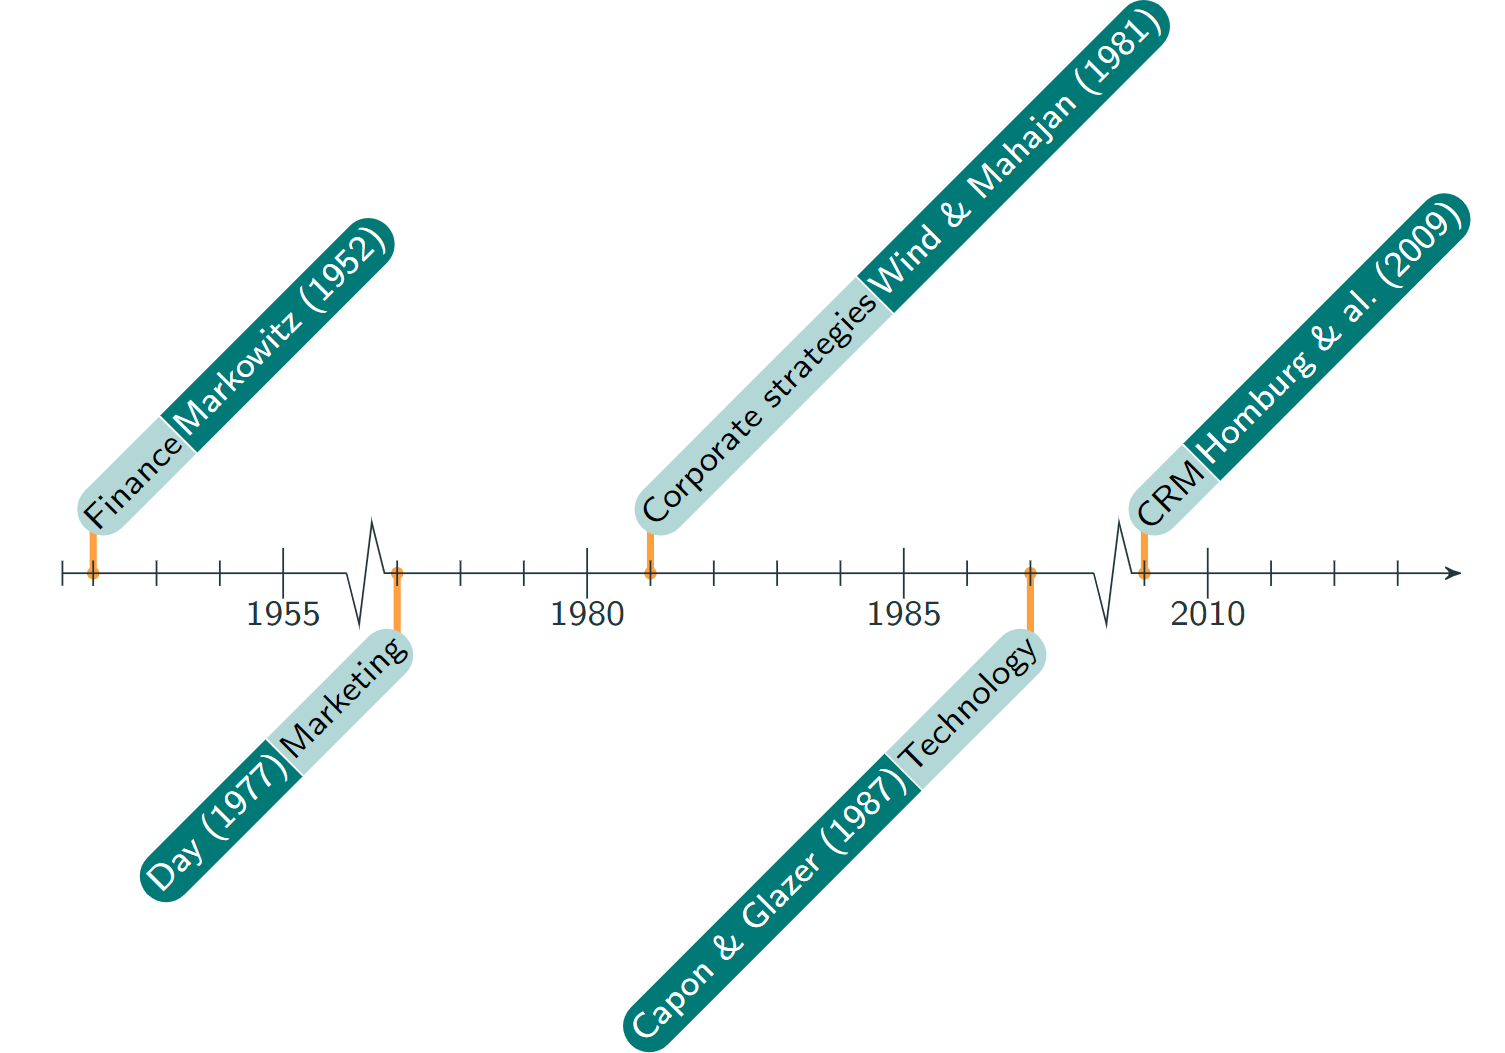
\includegraphics[width=400pt,height=300pt]{./imgs/portfolio_timeline} 

}

\caption{A timeline on the concept of portfolio}\label{fig:timeline}
\end{figure}

In their article \citet{CPM_CRM} examine how a company can define the
value of customers and segment these customers into \emph{portfolios}. They explain how segmentation leads to better understanding of the relative importance of each customer to the company's total profit. The authors consider a \emph{portfolio} segmented into four groups of clients: \emph{platinum}, \emph{gold}, \emph{silver} and \emph{bronze} customers. The \emph{portfolio} segmentation is based both on the cost to serve a client as well as the latter's \emph{value} to the firm, as depicted by figure \ref{fig:cpmmat}.

\begin{figure}

{\centering 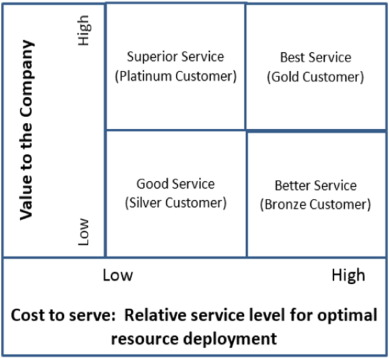
\includegraphics[width=300pt,height=300pt]{./imgs/cpm_matrix} 

}

\caption{Csutomer Portfolio Management (CPM) Matrix}\label{fig:cpmmat}
\end{figure}

According to this repartition into four main groups, Thakur and Workman highlight three strategies the firm can launch in order to efficiently manage its \emph{portfolio}. \textbf{Retention} aims to induce \emph{platinum} customers into repeating their purchases as they have a large contribution to the firm's revenue. \textbf{Customer relationship development} can be used to encourage customers to advance and upgrade to a higher segment. Such a strategy can be efficient for customers with high preference for a certain product or those with potential to shift to higher margin products. Conversely, \textbf{customer elimination or filtering} strategies are set up by the firm to encourage bottom customers who cost more than they are worth to leave the \emph{portfolio}.

As said in the introduction, an interesting improvement of \emph{portfolio} analysis may be to add a temporal dimension to the models. \citet{MANAGING_DYNAMICS_CUSTOMER_PORTFOLIO} show that the dynamic approach minimizes the current bias of underestimating low-value clients and overestimating high-value ones.

\hypertarget{attrition}{%
\section{On attrition}\label{attrition}}

\emph{Attrition} or churn has become a buzzword these last years. Churn analysis can be seen as an economic problem for three main reasons. Firstly, customers are in some way the firm's more precious asset. Secondly, the firm's resources in terms of customer relationship management are limited, so an efficient allocation needs to be deployed. Thirdly churn being a risk the firm has to cope with, it leads to asymmetric information from the firm's side. With the development of advanced Econometrics and Data Science, several methods can be implemented in order to estimate churn.

On the one hand, survival models are helpful in measuring customer lifetime. In her thesis, \citet{SURV_METHODS_INSURANCE} applies duration analysis to model the behavior of customers from an insurance company with a threefold purpose:

\begin{itemize}
\tightlist
\item
  Identify factors influencing customer loyalty.
\item
  Estimate the remaining lifetime of a client who has subscribed to multiple policies and cancelled one of them.
\item
  Study the influence of covariates changing over time.
\end{itemize}

Her study is motivated by the importance of the insurer/policyholder relationship in a digitalized environment where the costs of searching for information are loawer and lower and the risk of \emph{attrition} consequently higher. The author develops a two-part methodology to address the study's problematic. She begins by solely selecting insureds with at least two policies. Then, she fits a logit model to predict whether a policyholder will cancel their policies at the same time (type 1) or sequentially (type 2). She finally applies duration models on type 2 clients to determine the remaining time until all their policies are cancelled.

On the other hand, machine learning classification algorithms can be used for churn detection as illustrated by the work of \citet{CHURN_INSURANCE}. Her objective is to develop a predictive model to detect customer churn in an insurance company while highlighting the key drivers of \emph{attrition}. The underlying goals of her research paper are both minimizing revenue loss caused by churn and boosting the firm's competitiveness. Using data on vehicle insurance policies, Bellani incorporates features on the policyholders, the vehicles, the insurance policies as well as marketing data to predict the churn indicator variable. After missing data imputation and dimensionality reduction, the author falls back on under-sampling to overcome the issue of unbalanced classes. There are indeed much more active than cancelled policies in the dataset. Her methodology works as follows:

\begin{itemize}
\tightlist
\item
  The set of active policies is divided into 7 groups equal in size to the number of cancelled policies.
\item
  For each group of active policies, classification models (logistic regression, random forest and neural network) are trained on a subset of the original dataset including all the cancelled policies as well as the concerned group of active ones.
\item
  For each model, the predictions are aggregated across the 7 subsets for the final prediction.
\item
  Model selection is made by the means of the Kappa performance metric.
\end{itemize}

Ultimately when a customer leaves the firm's portfolio, it may worth it to consider all possible outcomes for the reason he churned. For instance, a client might leave their telecom company because of a bad service quality, or because of too high a price. In this context, competing risk analysis can be introduced since its main interest is to determine the reason why the client churned. In their recent article, \citet{COMPETING_RISKS} try to predict both the likelihood of customer churn and the reasons for \emph{attrition} using customer service data from a Dutch TSP. They estimate duration and competing risk models. In the competing risk model, three possible output states are considered: Controllable risk, Uncontrollable risk and Unknown risk. Each type of risk is assumed independent from another which means a client cannot be at high risk for two risks simultaneously. Besides, the authors implement a Latent Dirichlet Allocation model (see \citet{LDA} for more details) to identify the main topics in a set of emails sent by customers to the service center. Six topics are discovered by the algorithm and each of them is then incorporated as explanatory variable into the models. These topic variables increase the performance of both standard duration models and competing risk models for Controllable and Unknown risks. According to Slof, Frasincar, and Matsiiako, \emph{``customers who churn due to the Controllable risk or due to the Unknown risk tend to call the customer service center with a specific problem, while customers who churn due to the Uncontrollable risk do not call the customer service center with a specific problem''}.

\hypertarget{value}{%
\section{On customer value}\label{value}}

In recent years, customer \emph{portfolio} management (CPM) has focused on optimizing clients' \emph{value} to the firm. The company's interest lies in knowing how much net benefit it can expect from a customer today. These expectations are then used to implement efficient marketing strategies to get the highest return on investment. To that end, two key metrics are estimated by firms: customer lifetime value (CLV) and customer equity (CE) (see part \ref{valuedef} in the introduction for definitions).

According to \citet{CLV_DEF}, CLV is a temporal variable defined as the revenue derived from a customer minus the cost to the firm for maintaining the relationship with this very customer. As shown by \citet{CLV_CONTEXT}, CLV modelling depends on the type of relationship a firm has with its clients. In a contractual relationship, customer defections are observed which means that longer lifetime means higher customer value. Conversely, when the relationship is non-contractual, uncertainty arises between the customer's purchase behavior and lifetime.

With the development of data collection tools, companies have lots of customer-level data (or customer transaction data) at their disposal to measure CLV \citep{CLV_NBD}. Consequently, different modelling approaches can be adopted in order to estimate customer \emph{value.}

Recency Frequency Monetary (RFM) models are considered the simplest strategy to measure CLV and customer loyalty \citep{CLV}. They aim at targeting specific marketing campaigns at specific groups of customers to improve response rates. RFM models consist in creating clusters of clients based on three variables:

\begin{itemize}
\tightlist
\item
  \emph{Recency} which is the time that has elapsed since customers' last activity with the firm.
\item
  \emph{Frequency} that is the number of times customers transacted with the brand in a particular period of time.
\item
  \emph{Monetary} that is to say the value of customers' prior purchases.
\end{itemize}

However, RFM models have a limited predictive power since they only predict clients' behavior for the next period.

In their article on CLV management, \citet{CLV_MEASUREMENT} draw the review of more advanced modelling techniques that can be implemented to estimate customers' \emph{value.} A popular method to estimate customer lifetime value is the negative binomial distribution (NBD) - Pareto \citep{CLV_NBD} which helps solving the lifetime uncertainty issue. The model takes past customer purchase behavior as input such as the number of purchases in a specific time window and the date of last transaction. Then the model outputs a repurchase probability as well as a transaction forecast for each individual. In Borle and Singh's research paper, a hierarchical bayesian model is implemented with a view to jointly predict customer's churn risk and spending pattern. Here, the main advantage of using a bayesian approach is to give priors on CLV's drivers. The study is based on data coming from a membership-based direct marketing company where firm/client relationships are non-contractual. In other words, the times of each customer joining the membership and terminating it are known once these events happen. Thus the implementation of a sophisticated estimation strategy is justified.

In our study, emphasize is placed on estimating the overall value of a customer \emph{portfolio}. The methodology we develop is based on a research paper written by our Econometrics teacher Alain Bousquet, whose goal is to provide tools for an efficient management of patent \emph{portfolios} \citep{BREVETS}. The main idea is to consider each patent as an asset with a related value which can generate income if this very patent is exploited. The author emphasizes the importance to focus on the \emph{portfolio}'s \textbf{variance} on top of its expected value. Specifically, he explains that the variability in the probability of success in the exploitation of patents leads to a decrease in the overall risk to which the \emph{portfolio} is exposed. This modelling approach can be transposed to customer \emph{portfolio} analysis with the customer's \emph{value} corresponding to the CLV and the probability of exploitation being the opposite of the risk of \emph{attrition}. In this context, CLV can be estimated either with techniques mentioned above or regression methods. The customer's risk of churn can be modelled with duration models or machine learning techniques as evoked in \ref{attrition}. With this econometric framework, it is expected that customer heterogeneity be a key factor in the total variance of the portfolio's \emph{value}.

\hypertarget{duration}{%
\chapter{Duration models}\label{duration}}

This chapter presents theoretical basis of the models that are used to model customer \emph{portfolios.} As customer lifetime in a \emph{portfolio} is usually represented by the time to churn, duration models are adapted to the data we have at our disposal. Thus, this part focuses on introducing standard survival techniques.

\hypertarget{definition}{%
\section{Definition}\label{definition}}

According to \citet{CAMERON_TRIVEDI}, duration models (also called survival models) aims at measuring the time spent in a certain state before transitioning to another state. In Econometrics,

\begin{itemize}
\tightlist
\item
  a \textbf{state} corresponds to the class in which an individual \(i\) is at time \(t\).
\item
  a \textbf{transition} is movement from one state to another.
\item
  a \textbf{duration} measures the time spent in a certain state and is also called a \textbf{spell} length.
\end{itemize}

Since measuring the time until the event is needed for multiple purposes, duration analysis is used in a variety of economic sectors as depicted by the following table.

\begin{longtable}[]{@{}cc@{}}
\toprule
Economic sector & Purpose \\
\midrule
\endhead
Macroeconomics & Length of unemployment spells \\
Insurance & Risk analysis to offer a segmented pricing \\
Engineering & Time until a device breaks down \\
Epidemiology & Survival time of a virus \\
\textbf{Churn analysis} & \textbf{Time until a customer leaves the portfolio} \\
\bottomrule
\end{longtable}

\hypertarget{censoring-and-truncation}{%
\section{Censoring and Truncation}\label{censoring-and-truncation}}

When dealing with survival data, some observations are usually \textbf{censored} meaning they are related to spells which are not completely observed. Duration data can also suffer from a selection bias which is called \textbf{truncation}.

\hypertarget{censoring-mechanisms}{%
\subsection{Censoring mechanisms}\label{censoring-mechanisms}}

\textbf{Left-censoring} occurs when the event of interest occurs before the beginning of the observation period. For example, an individual is included in a study of unemployment duration at \(t_0\). At that time he has already been unemployed for a period but he cannot recall exactly the duration of this period. If we observe that he finds a job again at \(t_1\), we can only deduce that the duration of unemployment is bigger than \(t_1-t_0\), this individual is consequently left-censored. Observation 2 on figure \ref{fig:censoring} is associated with a left-censored spell \citep{LIU_SCOR}.

A spell is considered \textbf{right-censored} when it is observed from time \(t_0\) until a censoring time \(t_c\) as illustrated by observation 4 on figure \ref{fig:censoring}. For instance, the lifetime related to a customer who has not churned at the end of the observation period is right-censored. Let us note \(X_i\) the duration of a complete spell and \(C_i\) the duration of a right-censored spell. We also note \(T_i\) the duration actually observed and \(\delta_i\) the censoring indicator such that \(\delta_i = 1\) if the spell is censored. Then \((t_1, \delta_1),\dots,(t_N, \delta_N)\) are the realizations of the following random variables:

\begin{equation}
  \begin{aligned}
  T_i & = \min(X_i, C_i) \\
  \delta_i & = \pmb{1}_{X_i > C_i}
  \end{aligned}
  \label{eq:censoring}
\end{equation}

\hypertarget{selection-bias}{%
\subsection{Selection bias}\label{selection-bias}}

Survival data suffers from a \textbf{selection bias} (or truncation) when only a sub-sample of the population of interest is studied. A customer entering the firm's \emph{portfolio} after the end of the study is said to be \textbf{right-truncated}, whereas a client who has left the \emph{portfolio} before the beginning of the study is considered \textbf{left-truncated}. Mathematically, a random variable \(X\) is truncated by a subset \(A \in \mathbb{R}^+\) if instead of \(\Omega(X)\), we solely observe \(\Omega(X)\bigcap A\). On figure \ref{fig:censoring}, the first and fifth observations suffers from a selection bias.

\begin{figure}

{\centering 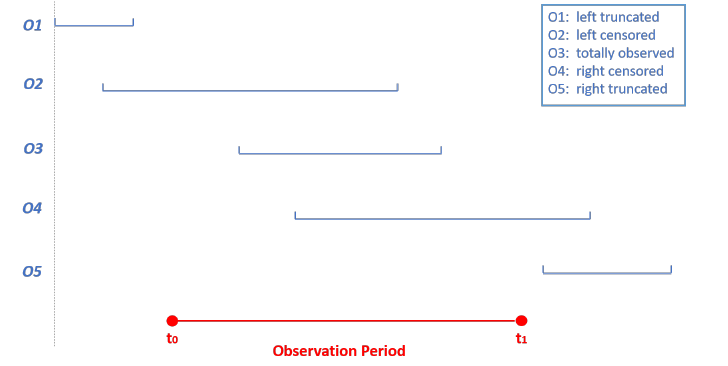
\includegraphics[width=500pt,height=250pt]{./imgs/censoring_and_truncation} 

}

\caption{Censored and truncated data}\label{fig:censoring}
\end{figure}

\hypertarget{probabilities}{%
\section{Probabilistic concepts}\label{probabilities}}

In survival analysis, the response variable denoted \(T\) is a time-to-event variable. Instead of estimating the expected failure time, survival models estimate the \textbf{survival} and \textbf{hazard rate} functions which depend on the realization of \(T\).

\hypertarget{survival-function}{%
\subsection{Survival function}\label{survival-function}}

The survival function \(S(t)\) represents the probability that the considered event occurs after time \(t\). For instance, \(S(t)\) can measure the probability that a given customer survives in the \emph{portfolio} at least until time \(t\). Mathematically, the survival function is defined as:
\begin{equation}
  S(t) = P(T > t) = 1 - F(t)
  \label{eq:survfun}
\end{equation}

where \(F(t)\) is the cumulative distribution function.

\begin{figure}

{\centering 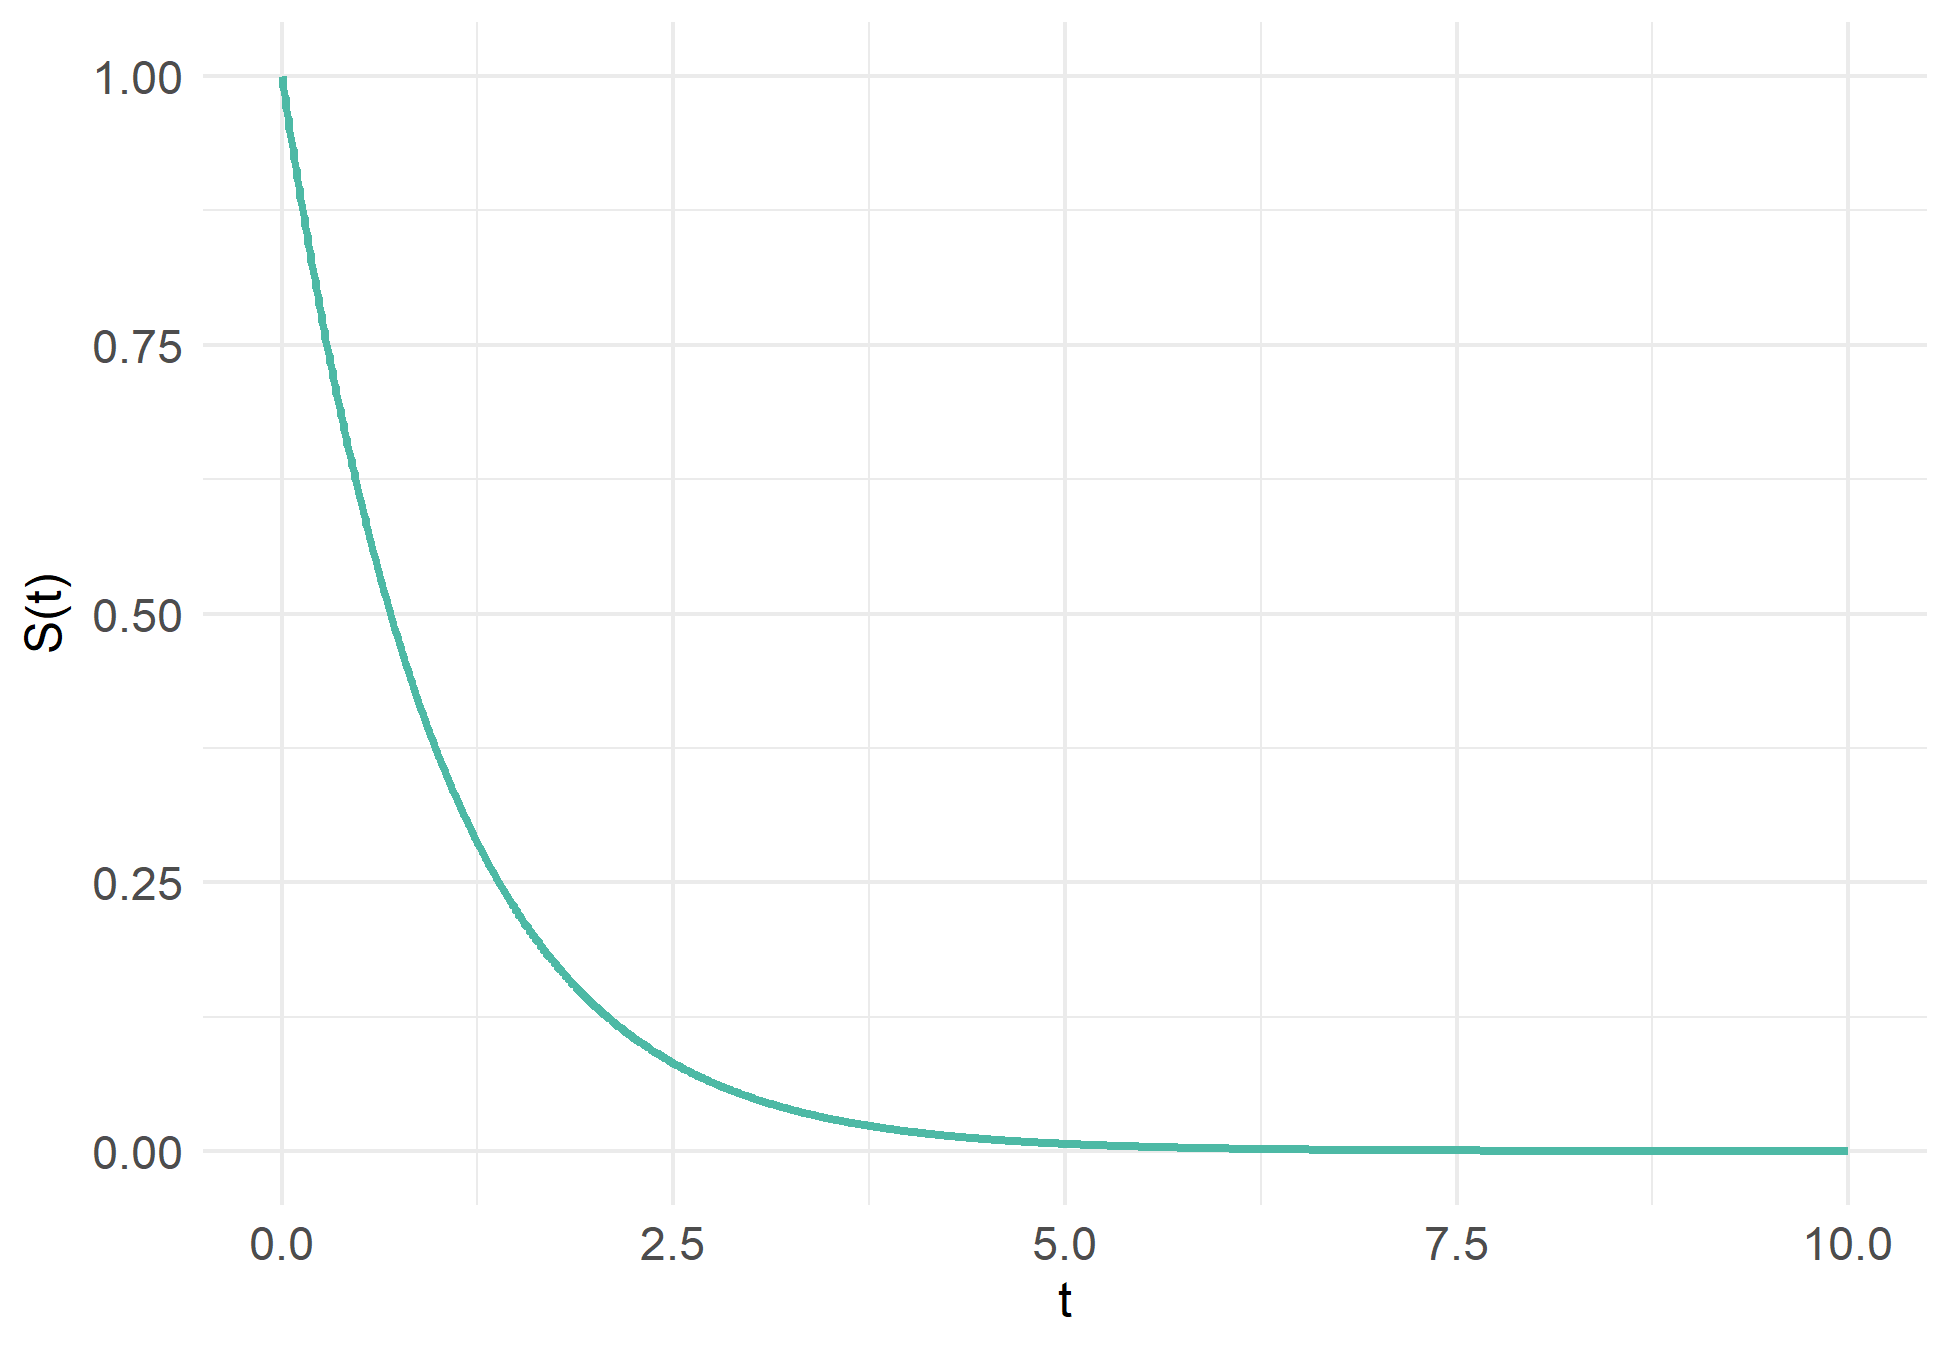
\includegraphics[width=400pt,height=300pt]{./imgs/surv_fun_plot} 

}

\caption{Survival function $S_T(t)$ with $T \sim \mathcal{E} (1)$}\label{fig:survfunplot}
\end{figure}

\hypertarget{hazard-and-cumulative-hazard-functions}{%
\subsection{Hazard and Cumulative Hazard functions}\label{hazard-and-cumulative-hazard-functions}}

Another key concept in duration analysis is the hazard function \(\lambda(t)\) which approximates the probability that the event occurs at time \(t\). For instance, \(\lambda(t)\) can measure the probability that a given individual leaves the firm \emph{portfolio} at time \(t\). Formally, it is expressed as follows:
\begin{equation}
  \lambda(t) = \lim_{\Delta t \to 0} \frac{P\big[t \leq T < t + \Delta t | T \geq t \big]}{\Delta t}
  \label{eq:hazfun}
\end{equation}

Using the Bayes formula, equation \eqref{eq:hazfun} can also be written as (see proof \eqref{eq:hazfunproof} in the appendix):
\begin{equation}
  \lambda(t) = \frac{-\text{d} \ln \big(S(t)\big)}{\text{d} t}
  \label{eq:hazfunbis}
\end{equation}

Finally, integrating the instantaneous hazard function gives the cumulative hazard function which can be more precisely estimated than the hazard function \citep{CAMERON_TRIVEDI} and is defined as:

\begin{equation}
  \Lambda (t) = \int_{0}^{t} \lambda(s) \text{d}s = - \ln \big(S(t)\big)
  \label{eq:cumhazfun}
\end{equation}

\begin{figure}

{\centering 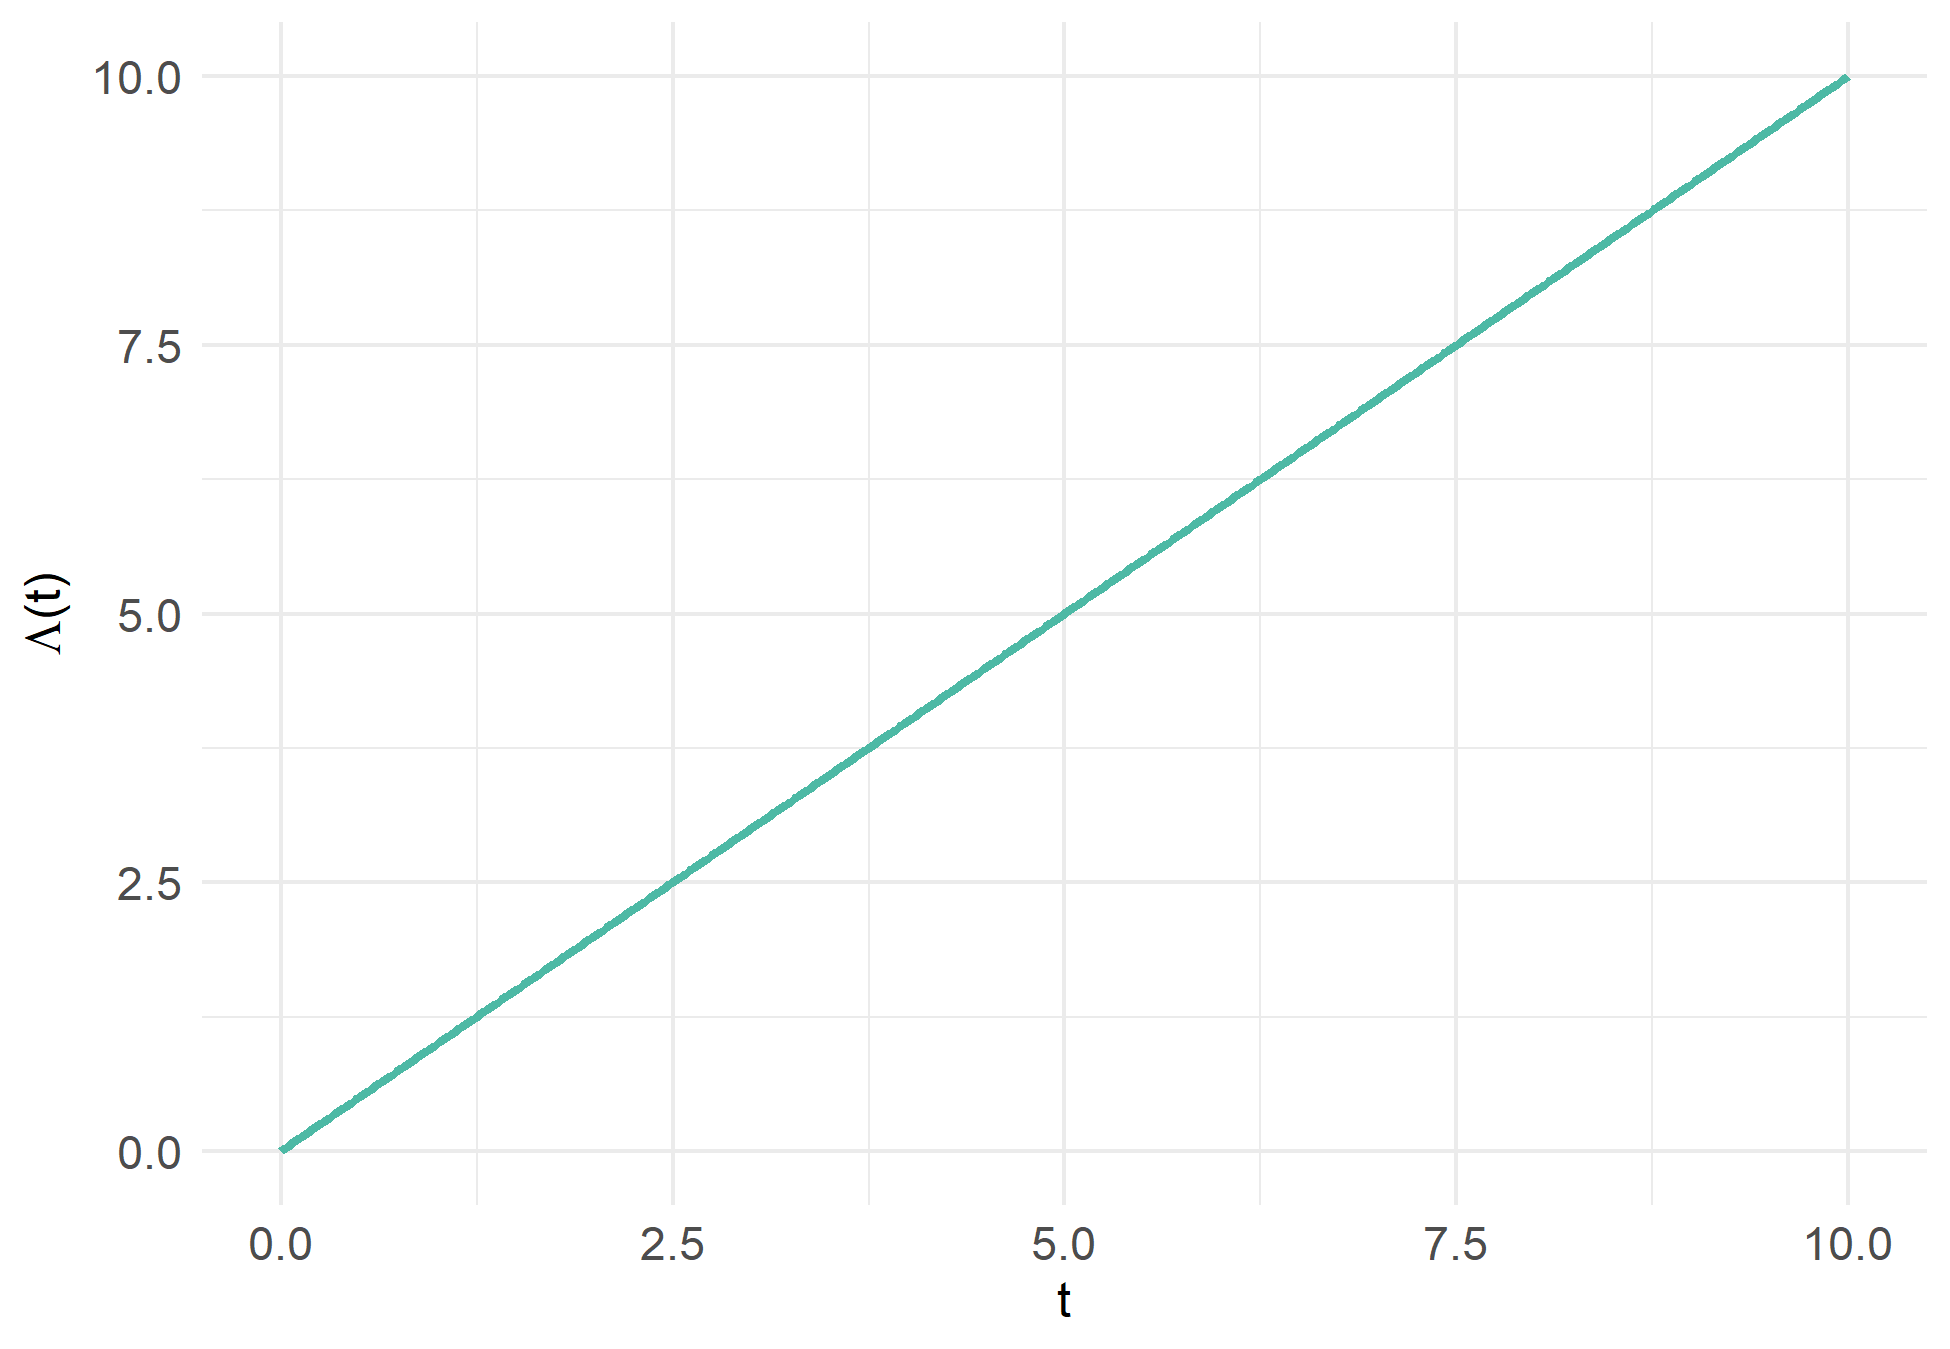
\includegraphics[width=400pt,height=300pt]{./imgs/cum_haz_plot} 

}

\caption{Cumulative Hazard function $\Lambda_T(t)$ with $T \sim \mathcal{E} (1)$}\label{fig:cumhazplot}
\end{figure}

Thus, \textbf{the hazard, survival and cumulative hazard functions} are three mathematical functions which describe the same distribution.

\hypertarget{nonparam}{%
\section{Nonparametric models}\label{nonparam}}

When dealing with duration data, these methods are helpful to have a general overview of the raw (or unconditional) hazard. Nonparametric models are rather used for data description than prediction. No explanatory variable is included in these models except for treatment variables such as the type of contract a customer has subscribed.

\hypertarget{notations}{%
\subsection{Notations}\label{notations}}

Let us consider a sample with \(N\) observations with \(k\) ordered discrete failure times (e.g.~a failure can be a churn event), such that \(\forall j \in [\![1; k]\!]\) :

\begin{itemize}
\tightlist
\item
  \(t_j\) the \(j^{\text{th}}\) discrete failure time,
\item
  \(d_j\) the number of spells terminating at \(t_j\),
\item
  \(m_j\) the number of right-censored spells in the interval \([t_j, t_{j+1}]\),
\item
  \(r_j\) the number of exposed durations right before time \(t_j\) i.e.~at time \(t_j^{-}\), such that:
  \begin{equation}
  r_j = (d_j + m_j) + \dots + (d_k + m_k) = \sum_{l|l \geq j} (d_l + m_l)
  \label{eq:exposed}
  \end{equation}
\end{itemize}

\hypertarget{hazard-function-estimator}{%
\subsection{Hazard function estimator}\label{hazard-function-estimator}}

As the instantaneous hazard at time \(t_j\) is defined as \(\lambda_j = P[T=t_j|T\geq t_j]\), a trivial estimator of \(\lambda_j\) is obtained by dividing the number of durations for which the event is realized at \(t_j\) by the total number of exposed durations at time \(t_j^{-}\). Formally, it is expressed as:

\begin{equation}
  \hat{\lambda}_j = \frac{d_j}{r_j}
  \label{eq:hazest}
\end{equation}

\hypertarget{kaplan-meier-estimator}{%
\subsection{Kaplan-Meier estimator}\label{kaplan-meier-estimator}}

Once the hazard function estimator computed, the discrete-time survivor function can be estimated using the Kaplan-Meier product-limit estimator. To estimate the survival at time \(t\), this estimator computes the joint probability that a spell stays in the same state until \(t\) (e.g.~remaining loyal to a firm until a certain time). This method is based on conditional probabilities and the survival function estimate is defined as:

\begin{equation}
  \hat{S}(t) = \Pi_{j|t_j \leq t} \big(1-\hat{\lambda}_j\big) = \Pi_{j|t_j \leq t}\frac{r_j - d_j}{r_j}
  \label{eq:kaplanmeier}
\end{equation}

When plotting the survival curve after having performed the Kaplan-Meier estimation, confidence bands are also added to the plot in order to reflect sampling variability \citep{CAMERON_TRIVEDI}. The confidence interval of the survival function \(\hat{S}(t)\) is derived from the estimate of the variance of \(S(t)\) which is obtained by the Grenwood estimate as in equation \eqref{eq:greenwood}.

\begin{equation}
  \widehat{\mathrm{V}}[\hat{S}(t)] = \hat{S}(t)^2 \sum_{j|t_j \leq t} \frac{d_j}{r_j(r_j-d_j)}
  \label{eq:greenwood}
\end{equation}

\hypertarget{nelson-aalen-estimator}{%
\subsection{Nelson-Aalen estimator}\label{nelson-aalen-estimator}}

The cumulative hazard function estimate is given by the Nelson-Aalen estimator which consists in summing up the hazard estimates for each discrete failure time.

\begin{equation}
  \hat{\Lambda}(t) = \sum_{j | t_j \leq t} \hat{\lambda}_{j} = \sum_{j | t_j \leq t} \frac{d_j}{r_j}
  \label{eq:nelsonaalen}
\end{equation}

Exponentiating \(\hat{\Lambda}(t)\), one can obtain a second estimate of the survival function (see proof \eqref{eq:linksurvcumhaz} in the appendix):

\begin{equation}
    \tilde{S}(t) = \exp \big( -\hat{\Lambda}(t) \big)
    \label{eq:survest}
\end{equation}

\hypertarget{parametric}{%
\section{Parametric models}\label{parametric}}

The nonparametric estimation is undoubtedly useful when it comes to have a general overview on the survival data. However, one may want to model the hazard and survivor functions with a functional form in which unknown parameters need to be optimized.

Parametric estimation has a twofold purpose that is to implement a robust model to estimate the risk that a specific event occurs while identifying the variables (or covariates) which best explain this risk.

When implementing parametric models, \(\lambda\), \(S\) and \(\Lambda\) are expressed based on the chosen parametric form. The instantaneous hazard function can either be constant or monotone.

In our study we assume that the explanatory variables are time-constant as we do not have dynamic data at our disposal. Thus, solely time-invariant duration models are presented.

\hypertarget{constant-hazard-exponential-model}{%
\subsection{Constant hazard (exponential model)}\label{constant-hazard-exponential-model}}

The exponential distribution models the time between events in a Poisson process and has the key property of being \emph{memoryless}. Let us note \(T\) a time-to-event variable such that \(T \sim \mathcal{E}(\theta)\) where \(\theta\) is the rate parameter. In this context, \emph{memorylessness} can be defined as follows:

\begin{equation}
  \mathbb{P}(T>t+s | T > t) = \mathbb{P}(T>s)
  \label{eq:memorylessness}
\end{equation}

\(\forall t \geq 0\ ,\ \theta > 0\) the density, hazard and survival functions can be expressed as:

\begin{equation}
  \begin{aligned}
    f_{\theta}(t) & = \theta e^{-\theta t} \\\\
    \lambda_{\theta}(t) & = \theta \\\\
    S_{\theta}(t) & = e^{-\theta t} \\\\
  \end{aligned}
  \label{eq:exponential}
\end{equation}

Thus, the exponential distribution is characterized by a \textbf{constant} hazard function which is a consequence of the \emph{memorylessness} property.

\hypertarget{monotone-hazard}{%
\subsection{Monotone hazard}\label{monotone-hazard}}

\hypertarget{weibull-model}{%
\subsubsection*{Weibull model}\label{weibull-model}}
\addcontentsline{toc}{subsubsection}{Weibull model}

The Weibull distribution is a less restrictive generalization of the exponential distribution defined by a shape parameter \(\nu\) and a scale parameter \(\theta\).

\(\forall t \geq 0\) and \(\nu,\ \theta > 0\) the density, hazard and survival functions can be expressed as:

\begin{equation}
  \begin{aligned}
      \lambda_{\nu,\theta}(t) & = \nu \bigg(\frac{1}{\theta}\bigg)^{\nu} t^{\nu - 1} \\\\
      S_{\nu, \theta}(t) & = \exp \Bigg( -\bigg(\frac{1}{\theta}\bigg)^{\nu} t\Bigg) 
  \end{aligned}
  \label{eq:weibull}
\end{equation}

The instantaneous hazard function \(\lambda_{\nu,\theta}\) is monotonic \textbf{decreasing} if \(\nu \in [0, 1]\). For instance, the \emph{attrition} risk may decrease as the customer's duration in the \emph{portfolio} increases. In this context, the client gets more and more loyal to the firm. If \(\nu=1\), the hazard rate is constant and \(T \sim \mathcal{E}(\theta)\). Converlsely, the hazard function is monotonic \textbf{increasing} if \(\nu > 1\). This can be the case when customers tend to continuously search for information on the firm's competitors, thus becoming more likely to churn as time goes by.

Figure \ref{fig:weibullplots} illustrates the hazard and survivor functions associated to a Weibull-distributed variable \(T\). The two curves' shape depend both on the shape (\(\nu\)) and scale (\(\theta\)) parameters. Some remarks can be made looking at the two plots. When \(\nu < 1\) the hazard function is decreasing meaning that the risk of the event occurring decreases as time goes by. When \(\nu > 1\) the hazard function is convex increasing which indicates that a marginal increase in time leads to an increase of over one unit in the the hazard function. The higher the shape parameter, the more increasing the hazard function. When \(\nu = \theta = 1\), it can be noted that the Weibull distribution corresponds to the exponential distribution (see figures \ref{fig:survfunplot} and \ref{fig:cumhazplot}).

\begin{figure}

{\centering 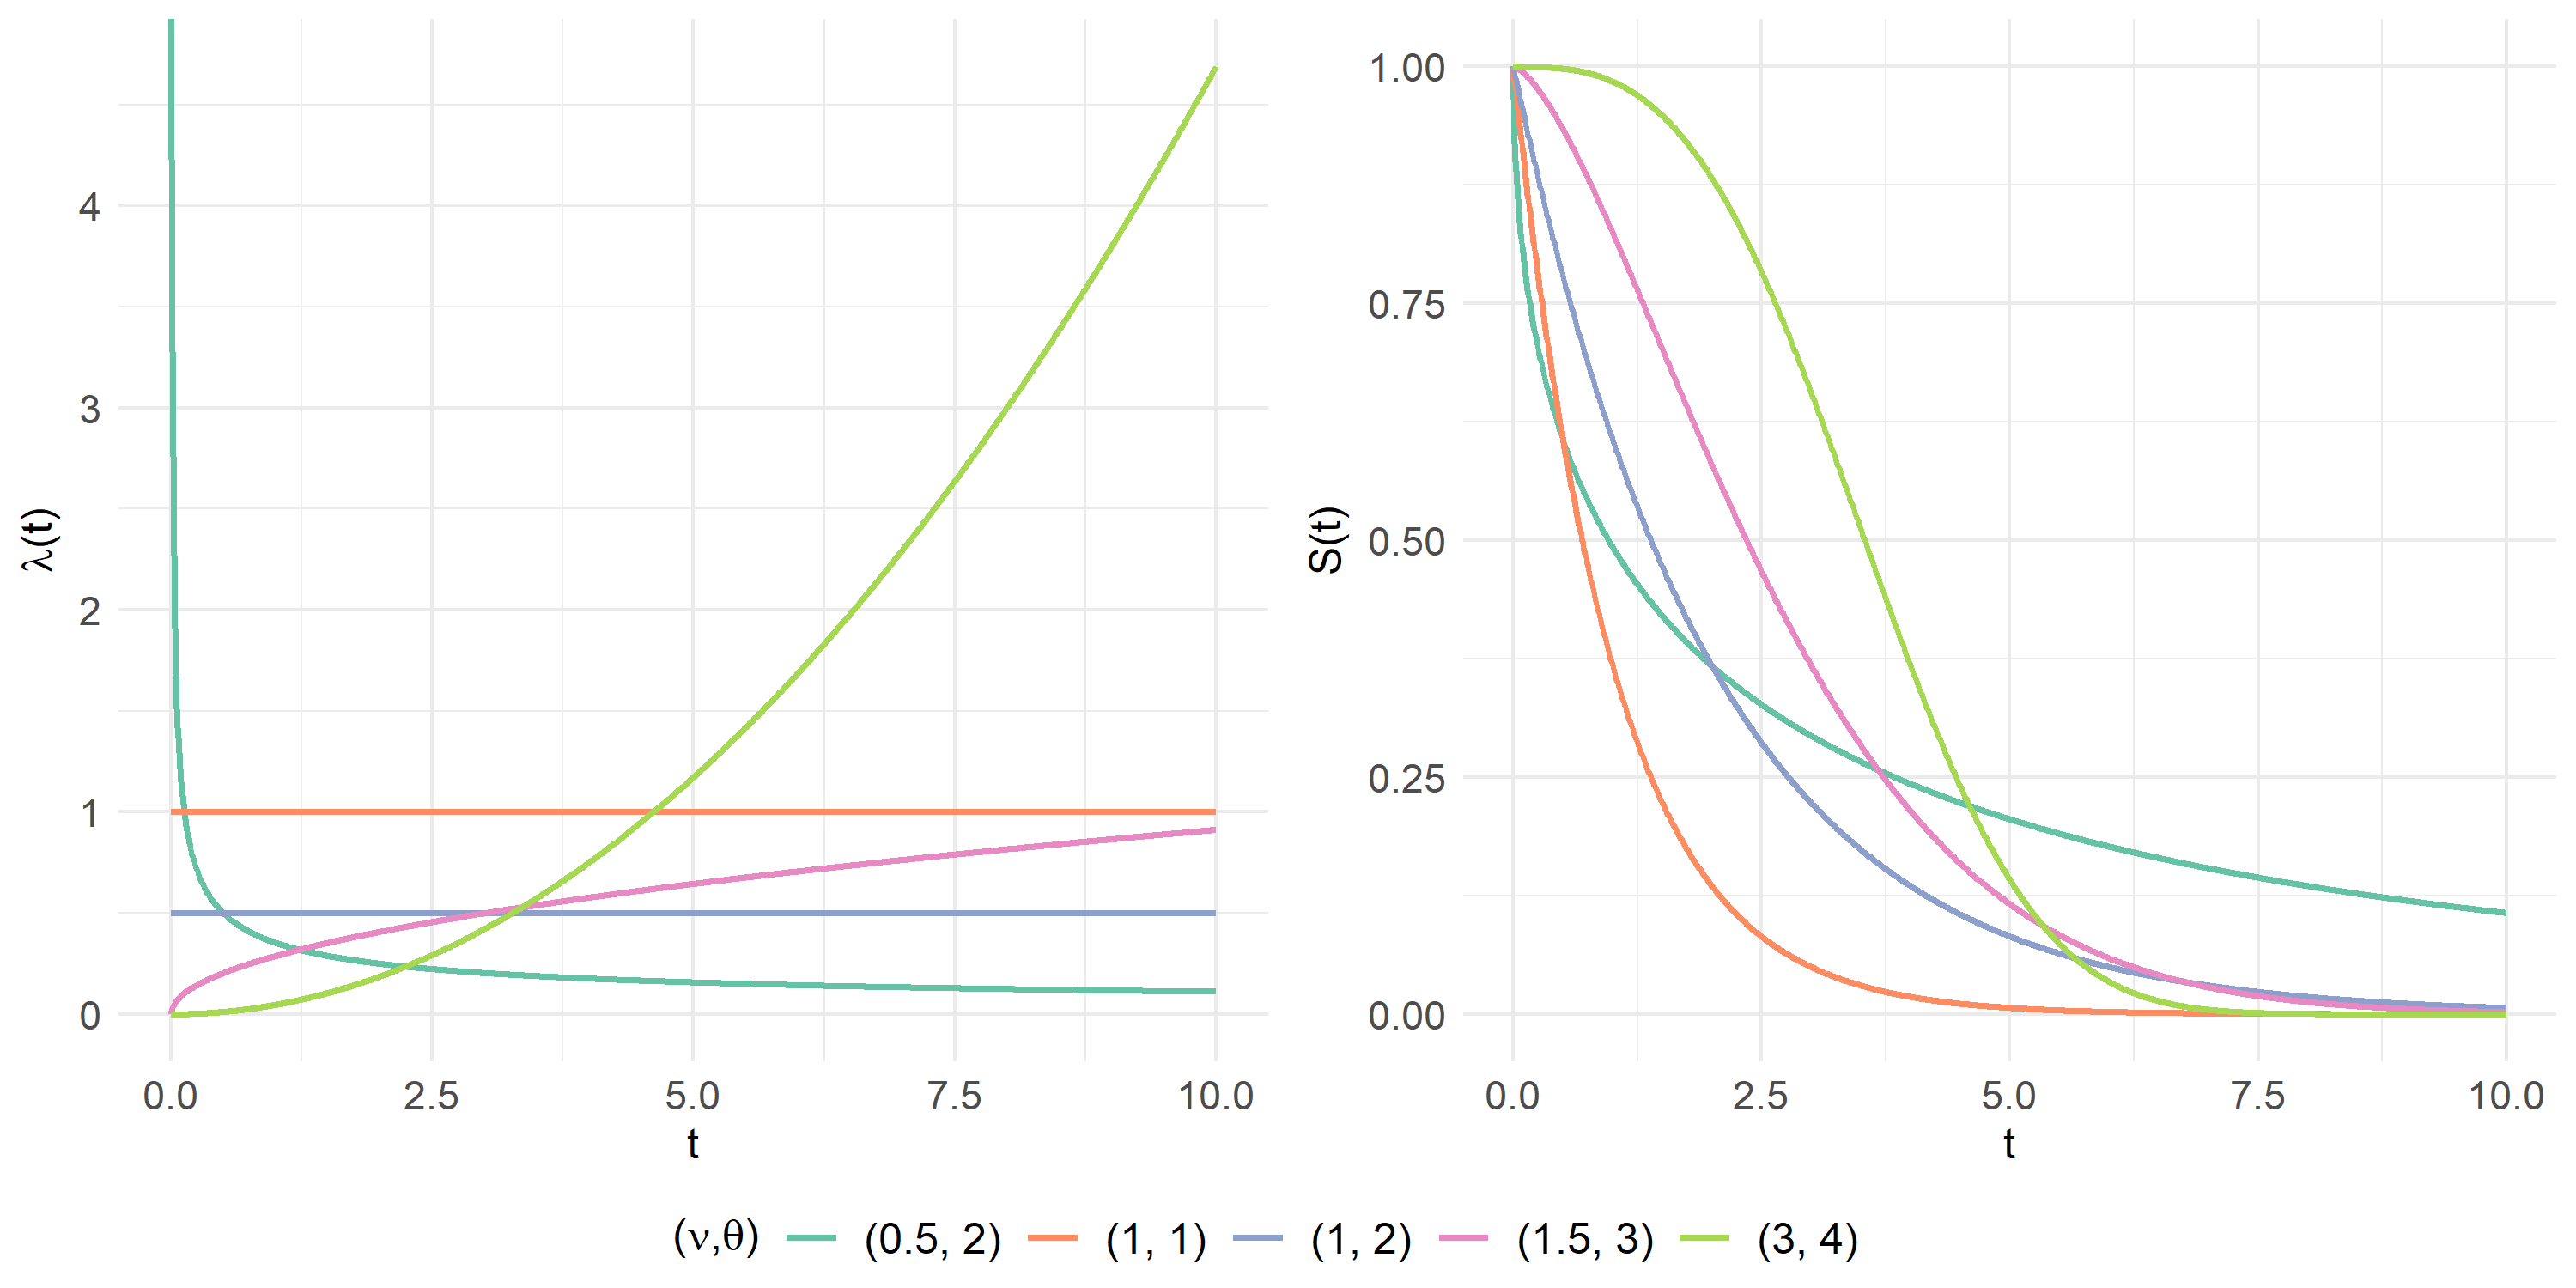
\includegraphics[width=700pt,height=350pt]{./imgs/weibull_plots} 

}

\caption{Hazard and Survival functions with $T \sim \mathcal{W} (\nu, \theta)$}\label{fig:weibullplots}
\end{figure}

\hypertarget{other-models}{%
\subsubsection*{Other models}\label{other-models}}
\addcontentsline{toc}{subsubsection}{Other models}

Different probabilistic distributions can be chosen to model the hazard and survival functions related to a time-to-event variable with monotone hazard. The Gompertz model is usually used for mortality data in biostatistics. As for the gamma model, it depends both on the gamma and inverse-gamma distributions and is also based on shape and scale parameters.

\hypertarget{concave-and-convex-hazard}{%
\subsection{Concave and convex hazard}\label{concave-and-convex-hazard}}

When the hazard function does not evolve in a monotonic fashion, the distributions introduced above are limited. The generalized Weibull model appears to be a good choice to estimate phenomena with concave or convex hazards. It is based on three parameters: \(\nu\) (shape), \(\theta\) (scale) and \(\gamma\). When \(\gamma = 1\), the generalized Weibull becomes the Weibull distribution \(\mathcal{W}(\nu, \theta)\).

\hypertarget{semi-parametric-estimation}{%
\section{Semi-parametric estimation}\label{semi-parametric-estimation}}

\hypertarget{proportional-hazards-models}{%
\subsection{\texorpdfstring{\emph{Proportional Hazards} models}{Proportional Hazards models}}\label{proportional-hazards-models}}

Parametric models assume that the baseline (or raw) hazard follows a specific distribution. This assumption can be sometimes too restrictive and semi-parametric models can be more adapted to describe the duration data.

In \emph{proportional hazards} (PH) models, the instantaneous risk function is \textbf{proportional} to the baseline hazard \(\lambda_0 (t,\alpha)\) modulo a \textbf{scaling factor} depending on the covariates \(\phi(\pmb{\mathrm{x}}, \beta)\). These models allow to generalize the basic survival models to a survival regression model which permits to take individuals' heterogeneity into consideration \citep{RMS}. The general mathematical formulation is expressed as follows:

\begin{equation}
    \lambda(t|\pmb{\mathrm{x}}) = \lambda_0 (t,\alpha)  \phi(\pmb{\mathrm{x}}, \beta) 
    \label{eq:ph}
\end{equation}

Note that when the function form of \(\lambda_0 (t,\alpha)\) is known, we are in the case of parametric estimation. For instance, the exponential, Weibull and Gompertz models are PH models since their respective hazards are function of some covariates.

\hypertarget{what-does-proportional-hazards-mean}{%
\subsubsection*{\texorpdfstring{What does \emph{proportional hazards} mean?}{What does proportional hazards mean?}}\label{what-does-proportional-hazards-mean}}
\addcontentsline{toc}{subsubsection}{What does \emph{proportional hazards} mean?}

PH models are said to be proportional as the relative hazard ratio between two individuals \(i\) and \(k\) does not vary over time, such that:

\begin{equation}
  \frac{\lambda(t|\mathrm{x_i})}{\lambda(t|\mathrm{x_k})} = \frac{\phi(\mathrm{x_i}, \beta) }{\phi(\mathrm{x_k}, \beta)}
  \label{eq:prophazratio}
\end{equation}

The formulation stated in equation \eqref{eq:prophazratio} needs to be verified when one wants to fit a PH model to real-life data and is only valid in the case of time-constant covariates.

\hypertarget{marginal-effects}{%
\subsubsection*{Marginal effects}\label{marginal-effects}}
\addcontentsline{toc}{subsubsection}{Marginal effects}

In \emph{proportional hazards} models, the marginal effect of covariate \(x_p\) on the hazard function can be easily derived since this computation only requires knowledge on \(\beta\). As shown in \citet{CAMERON_TRIVEDI}, a one-unit increase in the \(p^{\text{th}}\) covariate leads to the following variation in the hazard function \emph{ceteris paribus}:

\begin{equation}
    \frac{\partial \lambda(t|\pmb{\mathrm{x}}, \beta)}{\partial x_p} = \lambda(t|\pmb{\mathrm{x}}, \beta) \frac{\partial \phi(\pmb{\mathrm{x}}, \beta) / \partial x_p}{\phi(\pmb{\mathrm{x}}, \beta) }
    \label{eq:meph}
\end{equation}

Thus the new hazard after variation of the \(p^{\text{th}}\) covariate is the original hazard times the effect of \(x_p\) on the model's regression part.

\hypertarget{partial-likelihood-estimation}{%
\subsubsection*{Partial likelihood estimation}\label{partial-likelihood-estimation}}
\addcontentsline{toc}{subsubsection}{Partial likelihood estimation}

The vector of parameters \(\beta\) related to the regression part of the PH model is estimated by partial likelihood maximization. The method's principle consists in only estimating the regression's parameters \(\beta\) by considering the baseline hazard \(\lambda_0\) as noise. If desired an estimate of the baseline hazard can be recovered after estimation of \(\beta\) using, for instance, the Nelson-Aalen estimator (see part \ref{nonparam}). Cox's intuition is that no information can be retrieved from the intervals during which no event has occurred and that it is conceivable that \(\lambda_0\) is null in these intervals. Thus, solely the set of moments when an event occurs are considered in the estimation method.

In order to derive the partial likelihood function, let us note \(t_j\) the \(j^{\text{th}}\) discrete failure time in an \(N\)-sample with \(j \in [\![1; k]\!]\), such that:

\begin{itemize}
\tightlist
\item
  \(t_1 < t_2 < \dots < t_k\),
\item
  \(D(t_j) = \{l: t_l = t_j\}\) is the set of spells completed at \(t_j\) with \(\#D(t_j) = d_j\),
\item
  \(R(t_j) = \{l: t_l \geq t_j\}\) is the set of spells at risk at \(t_j\).
\end{itemize}

The contribution of a spell in \(D(t_j)\) to the likelihood function equals the conditional probability that the spell ends at \(t_j\) given it is exposed at that specific time and can be written as (see \citet{CAMERON_TRIVEDI} and proof \eqref{eq:contribpartiallikproof} for more details):

\begin{equation}
  \mathbb{P}\big[T_j = t_j | R(t_j) \big] = \frac{\phi(\mathrm{x_j}, \beta)}{\sum_{l \in R(t_j)} \phi(\mathrm{x_l}, \beta)}
  \label{eq:contribpartiallik}
\end{equation}

Given \(k\) discrete failure times are considered and that for each of those there is a set \(D(t_j)\) of completed spells, Cox defines the partial likelihood function as the joint product of the probability expressed in \eqref{eq:contribpartiallik}, such that:

\begin{equation}
  \mathcal{L}_p = \Pi_{j=1}^{k} \ \frac{\Pi_{m \in D(tj)} \ \phi(\mathrm{x_j}, \beta)}{\Big[\sum_{l \in R(t_j)} \phi(\mathrm{x_l}, \beta)\Big]^{d_j}}
  \label{eq:partlik}
\end{equation}

The latter formulation of the partial likelihood function is explained in more details in proofs \eqref{eq:partlikproof} and \eqref{eq:partlikproofbis} in the appendix.

\hypertarget{coxph}{%
\subsection{Cox PH model}\label{coxph}}

The Cox \emph{proportional hazards} model is the most popular for the analysis of duration data. This model is said to be semi-parametric as it makes no assumption regarding the nature of the baseline hazard function \(\lambda_0(t)\). The parametric part only relies in the modelling of the effect of some covariates on the hazard function \(\lambda(t)\). The relationship between the vector of covariates and the log hazard is linear and the parameters can be estimated by maximizing the partial likelihood function. The Cox PH model solely assumes that predictors act multiplicatively on the hazard function. The model is formulated as in equation \eqref{eq:ph} with the exponential function as link between the hazard and the covariates i.e.~\(\lambda(t|\pmb{\mathrm{x}}) = \lambda_0 (t,\alpha) \text{e}^{\pmb{\mathrm{x'}} \beta}\).

\hypertarget{mlsurv}{%
\section{Machine Learning for Survival Data}\label{mlsurv}}

In the previsous sections, some important models for duration data have been introduced. Here, emphasize is placed on machine learning algorithms that can also be implemented to predict a time-to-event variable such as the time to churn.

\hypertarget{survival-trees}{%
\subsection{Survival Trees}\label{survival-trees}}

Traditional decision trees, also called CART (Classification And Regression Trees), segment the feature space into multiple rectangles and then fit a simple model to each of these subsets as shown by figure \ref{fig:tree} \citep{ML_TREE}. The algorithm is a recursive partitioning which requires a criterion for choosing the \emph{best} split, another criterion for deciding when to stop the splits and a rule for predicting the class of an observation.

\begin{figure}

{\centering 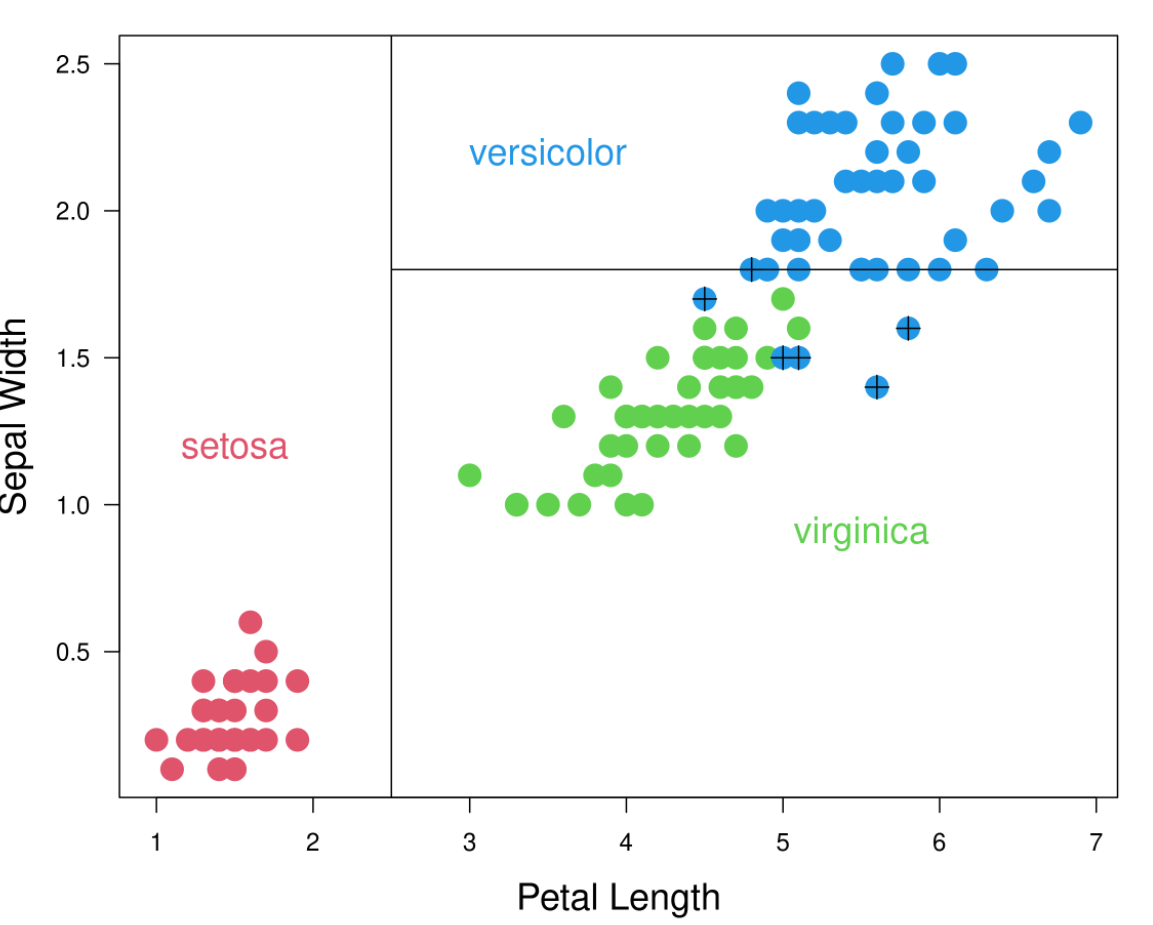
\includegraphics[width=0.45\linewidth,height=260pt]{./imgs/tree1} 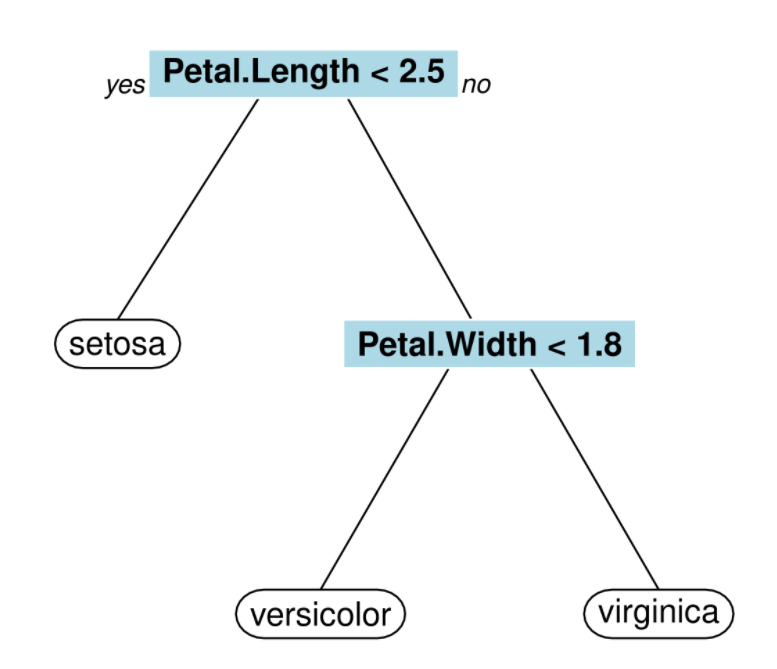
\includegraphics[width=0.45\linewidth,height=260pt]{./imgs/tree2} 

}

\caption{Clasification decision tree}\label{fig:tree}
\end{figure}

Survival tree \citep{SURV_TREE} is the adapted version of CART for duration data. The objective is to use tree based binary splitting algorithm in order to predict hazard rates. To that end, survival time and censoring status are introduced as response variables. The splitting criteria used for survival trees have the same purpose than the criteria used for CART that is to say maximizing between-node heterogeneity or minimizing within-node homogeneity. Nonetheless, node purity is different in the case of survival trees as a node is considered pure if all spells in that node have similar survival duration. The most common criterion is the \textbf{logrank test} statistic to compare the two groups formed by the children nodes. For each node, every possible split on each feature is being examined. The best split is the one maximizing the survival difference between two children nodes. The test statistic is \(\chi^2\) distributed which means the higher its value, the higher between-node variability so the better the split. Let \(t_1, \dots, t_k\) be the \(k\) ordered failure times. At the \(j^{\text{th}}\) failure time, the logrank statistic is expressed as \citep{SEGAL}:

\begin{equation}
  \chi^2_{\text{logrank}} = \frac{\big[\sum_{j=1}^k \ (d_{0j} - r_{0j} \times d_j/r_j) \big]^2}{\sum_{j=1}^k \ \frac{r_{1j}r_{0j}d_j(r_j - d_j)}{r_j^2(r_j -1)}}
  \label{eq:logrank}
\end{equation}

\hypertarget{random-survival-forests-rsf}{%
\subsection{Random Survival Forests (RSF)}\label{random-survival-forests-rsf}}

This algorithm is proposed by \citet{RSF} and is an ensemble of decision trees for the analysis of right-censored survival data. As random forests used for regression and classification, RSF are based on \textbf{bagging} which implies that \(B\) bootstrap samples are drawn from the original data with 63\(\%\) of them in the bag data and the remaining part in the out-of-bag (OOB) data. For each bootstrap sample, a survival tree is grown based on \(p\) randomly selected features. Then, the parent node is split using the feature among the selected ones that maximizes survival difference between children nodes. Each tree is grown to full size and each terminal node needs to have no less than \(d_0\) unique events. The cumulative hazard function (CHF) is computed for each tree using the Nelson-Aalen estimator such as:

\begin{equation}
  \widehat{H_l}(t) = \sum_{t_{j, l} < t} \frac{d_{j,l}}{r_{j,l}}
  \label{eq:chf}
\end{equation}

where \(t_{j,l}\) is the \(j^{\text{th}}\) distinct event time in leaf \(l\), \(d_{j,l}\) the number of events completed at \(t_{j,l}\) and \(r_{j,l}\) the number of spells at risk at \(t_{j,l}\).

All the CHFs are then averaged to obtain the bootstrap ensemble CHF and prediction error is finally computed on the OOB ensemble CHF.

\hypertarget{cox-boosting}{%
\subsection{Cox Boosting}\label{cox-boosting}}

\textbf{Boosting} is an ensemble method which combines several weak predictors into a strong predictor. The idea of most boosting methods is to train predictors sequentially, each trying to correct its predecessor. Cox boosting \citep{COX_BOOSTING} is designed for high dimension survival data and has the purpose of feature selection while improving the performance of the standard Cox model. The key difference with gradient boosting is that Cox boosting does not update all coefficients at each boosting step, but only updates the coefficient that improves the overall fit the most. The loss function is a penalized version of the Cox model's log-likelihood (see equation \eqref{eq:partlik} for the likelihood function of the Cox model). Cox boosting helps measuring variable importance as the coefficients associated to more representative variables will be updated in early steps.

\hypertarget{performance-metrics}{%
\section{Performance metrics}\label{performance-metrics}}

\hypertarget{concordance-index-c-index}{%
\subsection{Concordance index (C-index)}\label{concordance-index-c-index}}

C-index is a goodness of fit measure for models which produce risk scores. It is commonly used to evaluate risk models in survival analysis, where data may be censored.

Consider both the observations and prediction values of two instances \((y_1; \hat{y}_1)\) and \((y_2; \hat{y}_2)\). \(y_i\) and \(\hat{y}_i\) represent respectively the actual observation time and the predicted time. Mathematically, the C-index is defined as the probability to well predict the order of event occurring time for any pair of instances.

\begin{equation}
  c = \mathbb{P}\big(\hat{y}_1 > \hat{y}_2 | y_1 > y_2\big)
  \label{eq:cindex}
\end{equation}

Another way to write the C-index metric is to compute the ratio between concordant pairs and the total number of pairs. Consider individual \(i\) and let \(T\) be the time-to-event variable and \(\eta_i\) the risk score assigned to \(i\) by the model. We say that the pair \((i, j)\) is a concordant pair if \(\eta_i > \eta_j\) and \(T_i < T_j\), and it is a discordant pair if \(\eta_i > \eta_j\) and \(T_i > T_j\). If both \(T_i\) and \(T_j\) are censored, then this pair is not taken into account in the computation. If \(T_j\) is censored, then:

\begin{itemize}
\tightlist
\item
  If \(T_j < T_i\) the pair \((i, j)\) is not considered in the computation since the order cannot be determined.
\item
  If \(T_j > T_i\), the order can be determined and \((i, j)\) is concordant if \(\eta_i > \eta_j\), discordant otherwise.
\end{itemize}

Equation \eqref{eq:cindex} can then be rewritten as follows:

\begin{equation}
\begin{aligned}
c & = \frac{\# \text{concordant pairs}}{\# \text{concordant pairs} + \# \text{discordant pairs}} \\\\
c & = \frac{\sum_{i \neq j} \pmb{1}_{\eta_i < \eta_j} \pmb{1}_{T_i > T_j}d_j}{\sum_{i \neq j} \pmb{1}_{T_i > T_j}d_j}
\end{aligned}
\label{eq:cindex2}
\end{equation}

with \(d_j\) the event indicator variable.

The concordance index ranges between 0 and 1. A C-index below 0.5 indicates a very poor model. A C-index of 0.5 means that the model is rather a non-informative model making random predictions. A model with C-index 1 makes perfect prediction. Generally, a C-index higher than 0.7 indicates a good performance.

\hypertarget{brier-score}{%
\subsection{Brier score}\label{brier-score}}

The Brier score is another statistical metric for evaluating duration models' performance and is defined as the mean squared error between the estimated survival probability and the observed survival at time \(t\):

\begin{equation}
  BS(t) = \frac{1}{N} \sum_{i=1}^{N} \Big(\pmb{1}_{\{t_i>t\}} - \hat{S}(t|\mathrm{x}_i) \Big)^2
  \label{eq:brier}
\end{equation}

The Cox \emph{proportional hazards} model is the most popular for the analysis of duration data. This model is said to be semi-parametric as it makes no assumption regarding the nature of the baseline hazard function \(\lambda_0(t)\). The parametric part only relies in the modelling of the effect of some covariates on the hazard function \(\lambda(t)\). The relationship between the vector of covariates and the log hazard is linear and the parameters can be estimated by maximizing the partial likelihood function. The Cox PH model solely assumes that predictors act multiplicatively on the hazard function. The model is formulated as in equation \eqref{eq:ph} with the exponential function as link between the hazard and the covariates i.e.~\(\lambda(t|\pmb{\mathrm{x}}) = \lambda_0 (t,\alpha) \text{e}^{\pmb{\mathrm{x'}} \beta}\).

\hypertarget{dataMining}{%
\chapter{Data Mining methods}\label{dataMining}}

While the previous chapter introduces the fundamentals related to survival analysis, this part focuses on data mining techniques used in our modelling approach. On the on hand, multiple correspondence analysis is introduced as it is used in the following chapter with a view of converting categorical features into continuous principal axes. On the other hand, this section centers on unsupervised classification which is a useful method when it comes to segmentation.

\hypertarget{mutliple-correspondence-analysis-mca}{%
\section{Mutliple Correspondence Analysis (MCA)}\label{mutliple-correspondence-analysis-mca}}

\hypertarget{definition-1}{%
\subsection{Definition}\label{definition-1}}

Multiple Correspondence Analysis is a dimension reducing method which takes multiple categorical variables and seeks to identify associations between levels of those variables. MCA aims at highlighting features that separate classes of individuals, while determining links between variables and categories. To that end, MCA keeps the core information by the means of principal components which are projected axes \citep{MCA}.

\hypertarget{complete-disjunctive-table}{%
\subsection{Complete disjunctive table}\label{complete-disjunctive-table}}

MCA can be applied on data stored in a complete disjunctive table which is an indicator matrix.

\begin{figure}

{\centering 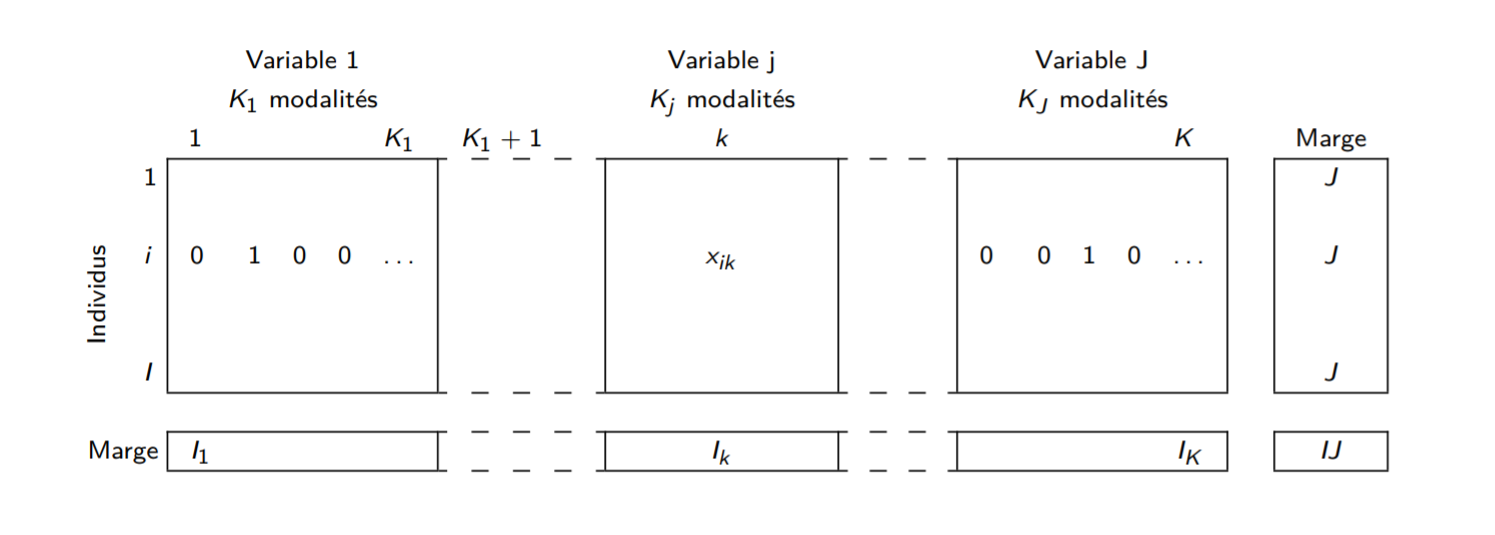
\includegraphics[width=20.76in]{./imgs/TDC} 

}

\caption{Complete disjunctive table}\label{fig:tdc}
\end{figure}

with,

\begin{itemize}
\tightlist
\item
  \(I\) the number of individuals,
\item
  \(J\) the number of variables,
\item
  \(K_j\) the number of categories in the \(j^{th}\) variable,
\item
  \(I_k\) the number of individuals with the \(k^{th}\) category.
\end{itemize}

\hypertarget{distances}{%
\subsection{Distances}\label{distances}}

The individuals' analysis processed by MCA relies on the distance between individuals which is computed as follows for 2 data points \(i\) and \(l\):

\begin{equation}
  d^2(i;l) = \frac{1}{J}\sum_{k=1}^K \frac{I}{I_k}(x_{ik} - x_{lk})^2
  \label{eq:mcaDist1}
\end{equation}

The distance between two categories \(j\) and \(k\) allows to determine how close they are and is calculated as follows:

\begin{equation}
  d^2(j;k) = \frac{I}{I_k I_j}\times I_{k\neq j}
  \label{eq:mcaDist2}
\end{equation}

with \(I_{k\neq j}\) the number of individuals with one and only one of the \(j\) or \(k\) categories.

\hypertarget{algorithm}{%
\subsection{Algorithm}\label{algorithm}}

\begin{enumerate}
\def\labelenumi{\arabic{enumi}.}
\tightlist
\item
  The axes' origin is placed at the individuals point cloud's barycenter;
\item
  A sequence of orthogonal axes is seeked so as to maximize the data's projected inertia;
\item
  These orthogonal projections are represented onto a plan made up of principal components, \((F_1, F_2)\) being the first projected plan.
\end{enumerate}

\hypertarget{unsupervised-classification}{%
\section{Unsupervised classification}\label{unsupervised-classification}}

Clustering is an unsupervised learning technique that groups similar data points such that the points in the same group are more similar to each other than the points in the other groups. The group of similar data points is called a cluster. It is said to be unsupervised as the groups are not labeled but discovered by the algorithm. Consequently, it may not be possible to find separate clusters of data points.

\hypertarget{hierarchical-clustering-on-principal-components-hcpc}{%
\subsection{Hierarchical Clustering on Principal Components (HCPC)}\label{hierarchical-clustering-on-principal-components-hcpc}}

The HCPC approach combines the three standard methods used in multivariate data analysis:

\begin{itemize}
\tightlist
\item
  Principal Components methods such as MCA,
\item
  Agglomerative hierarchical clustering,
\item
  Consolidation by k-means partitioning.
\end{itemize}

\hypertarget{agglomerative-hierarchical-clustering-ahc}{%
\subsection{Agglomerative Hierarchical Clustering (AHC)}\label{agglomerative-hierarchical-clustering-ahc}}

\hypertarget{algorithm-1}{%
\subsubsection*{Algorithm}\label{algorithm-1}}
\addcontentsline{toc}{subsubsection}{Algorithm}

\begin{enumerate}
\def\labelenumi{\arabic{enumi}.}
\tightlist
\item
  Each data point is initially considered an individual cluster;
\item
  Compute the proximity matrix which represents the distances, taken pairwise, between the elements of a set;
\item
  Merge the two closest clusters and update the proximity matrix until only a single cluster remains.
\end{enumerate}

\hypertarget{distance-between-two-observations}{%
\subsubsection*{Distance between two observations}\label{distance-between-two-observations}}
\addcontentsline{toc}{subsubsection}{Distance between two observations}

The choice of the distance metric is a critical step in clustering. It defines how the similarity of two elements \((x, y)\) is calculated and it will influence the shape of the clusters. There are several distance measures such as \emph{Euclidean}, \emph{Manhattan}, \(\chi^2\), etc. In our study the classical \emph{Euclidean} distance metric is chosen and is defined as follows:

\begin{equation}
  d_{euc}(x,y) = \sqrt{\sum_{i=1}^n(x_i - y_i)^2}
  \label{eq:euclidean}
\end{equation}

\hypertarget{similarities-between-clusters---ward-method}{%
\subsubsection*{Similarities between clusters - Ward method}\label{similarities-between-clusters---ward-method}}
\addcontentsline{toc}{subsubsection}{Similarities between clusters - Ward method}

Calculating the similarity between two clusters is determining to merge the clusters. Here, the Ward method \citep{UNSUPERVISED_CLASSIF} is chosen and it consists in merging groups which drive down as little as possible the within inertia, ie the homogeneity of clusters. Mathematically, Ward criterion is defined as follows:

\begin{equation}
  \Delta (A, B) = \frac{1}{n} \times \frac{n_A n_B}{n_A + n_B}d^2(g_A, g_B)
  \label{eq:ward}
\end{equation}

with \(g_A\) et \(g_B\) the clusters' barycenters (the mean point) et \(n_A\) et \(n_B\) the clusters' frequencies.

Ward method needs to be minimized and tends to group together clusters which are close to each other in terms of barycenters, as well as small frequency clusters.

Ward method leads to choose the optimal number of clusters. Let \(\Delta k\) be the increase in within inertia when going from \(k+1\) groups to \(k\) groups. Then, the proper number of classes \(k^*\) can be such that \(\frac{\Delta k-1}{\Delta k}\) is as little as possible.

\hypertarget{the-k-means-algorithm}{%
\subsection{The k-means algorithm}\label{the-k-means-algorithm}}

\(k\) data points are chosen as initial centers.The following steps are repeated until the clusters identified are homogeneous enough or until a fixed number of iterations:

\begin{enumerate}
\def\labelenumi{\arabic{enumi}.}
\tightlist
\item
  The distances between the data points and the centers are computed;
\item
  Each data point is assigned to the nearest center, ;
\item
  The \(k\) previous centers are replaced by the barycenters of the \(k\) classes identified during the previous step.
\end{enumerate}

\hypertarget{data}{%
\chapter{Data}\label{data}}

In this chapter, we introduce the \href{https://www.kaggle.com/yeanzc/telco-customer-churn-ibm-dataset}{kaggle} dataset related to customers of a fictional telecommunications service provider (TSP). In this duration dataset, the \texttt{Churn\_Value} status variable indicates whether the customer left the firm's \emph{portfolio} within the last month while the \texttt{Tenure\_Months} variable stands for the duration actually observed. Besides customer \emph{value} can be approximated by the \texttt{CLTV} variable.

\hypertarget{general-overview}{%
\section{General Overview}\label{general-overview}}

The data set used in this study contains 29 variables and 7032 customers from a telecom firm. For each client, the data includes:

\begin{itemize}
\item
  \textbf{Demographic} information: \texttt{CustomerID}, \texttt{City}, \texttt{Zip\_Code}, \texttt{Latitude}, \texttt{Longitude}, \texttt{Gender}, \texttt{Senior\_Citizen}, \texttt{Partner} and \texttt{Dependents}.
\item
  \textbf{Customer account} information: \texttt{Tenure\_Months}, \texttt{Contract}, \texttt{Paperless\_Billing}, \texttt{Payment\_Method}, \texttt{Monthly\_Charges}, \texttt{Total\_Charges}, \texttt{Churn\_Label}, \texttt{Churn\_Value}, \texttt{Churn\_Score}, \texttt{CLTV}, \texttt{Churn\_Reason}.
\item
  \textbf{Services} information: \texttt{Phone\_Service}, \texttt{Multiple\_Lines}, \texttt{Internet\_Service}, \texttt{Online\_Security}, \texttt{Online\_Backup}, \texttt{Device\_Protection}, \texttt{Tech\_Support}, \texttt{Streaming\_TV}, \texttt{Streaming\_Movies}.
\end{itemize}

\begin{table}[H]

\caption{\label{tab:dataoverview}Interesting variables for the 5 first customers in the data set}
\centering
\begin{tabular}[t]{rrlrr}
\toprule
CustomerID & Monthly\_Charges & Internet\_Service & Tenure\_Months & Churn\_Value\\
\midrule
\cellcolor{gray!6}{1} & \cellcolor{gray!6}{53.85} & \cellcolor{gray!6}{DSL} & \cellcolor{gray!6}{2} & \cellcolor{gray!6}{1}\\
2 & 70.70 & Fiber optic & 2 & 1\\
\cellcolor{gray!6}{3} & \cellcolor{gray!6}{99.65} & \cellcolor{gray!6}{Fiber optic} & \cellcolor{gray!6}{8} & \cellcolor{gray!6}{1}\\
4 & 104.80 & Fiber optic & 28 & 1\\
\cellcolor{gray!6}{5} & \cellcolor{gray!6}{103.70} & \cellcolor{gray!6}{Fiber optic} & \cellcolor{gray!6}{49} & \cellcolor{gray!6}{1}\\
\addlinespace
6 & 55.20 & DSL & 10 & 1\\
\bottomrule
\end{tabular}
\end{table}

As shown by table \ref{tab:dataoverview}, the \texttt{Churn\_Value} status variable indicates whether the customer left the firm's \emph{portfolio} within the last month and \texttt{Tenure\_Months} is the duration variable.

Since the purpose of our study relies in estimating the overall value of this fictional firm's \emph{portfolio}, two groups of target variables can be considered. On the one hand \texttt{Churn\_Value} and \texttt{Tenure\_Months} permit to determine whether a customer is active in the \emph{portfolio}. They are used as response variables in the survival models. On the other hand, \texttt{Monthly\_Charges} variable indicates the price paid by customers each month and may be used to derive a customer raw value. Even though the \texttt{CLTV} variable represents each customer's \emph{value} through measurement of customer lifetime value, we do not have any information on its calculation. Thus, it is not used in the model developed in the next chapter.

\hypertarget{churndescstats}{%
\section{\texorpdfstring{\texttt{Churn\_Value} and \texttt{Tenure\_Months}}{Churn\_Value and Tenure\_Months}}\label{churndescstats}}

As the combination of these two features form the response variable in the duration models, a relevant approach to have an overall description of the risk of \emph{attrition} may be to draw the raw survival curves depending on treatment variables. Pearson's \(\chi^2\) tests are also performed so as to test the statistical relationships between the churn indicator variable and explanatory features. Pearson's \(\chi^2\) test determines whether there is a statistically significant difference between the expected frequencies and the observed frequencies in one or more categories of a contingency table. It is thus adapted to test whether two categorical variables are statistically independent. In this context, it appears interesting to use explanatory features related demographic, customer account and services subscribed as treatment variables when fitting the Kaplan-Meier estimator and implementing the tests.

\hypertarget{demographic-data}{%
\subsection*{Demographic data}\label{demographic-data}}
\addcontentsline{toc}{subsection}{Demographic data}

Table \ref{tab:chi2demographics} depicts the \(\chi^2\) tests' results performed on demographic variables. Given the \emph{p-values} are ranked in ascending order and given the lower the \emph{p value} the stronger link between two categorical variables, \texttt{Dependents} appears to be the most correlated feature with \texttt{Churn\_Label}. When comparing this result with the corresponding survival plot in figure \ref{fig:kmdemographics}, it can be noted that customers with dependants have a longer lifetime in the \emph{portfolio}. Conversely, \texttt{Gender} and \texttt{Churn\_Label} are statistically independent as stated by the high test's \emph{p value} (\(\approx .49\)).

\begin{table}[H]

\caption{\label{tab:chi2demographics}Independence $\chi^2$ test between churn and demographic variables}
\centering
\begin{tabular}[t]{lrrrl}
\toprule
  & Statistic & Df & Critical Value & p-value\\
\midrule
\cellcolor{gray!6}{Dependents} & \cellcolor{gray!6}{431.65} & \cellcolor{gray!6}{1} & \cellcolor{gray!6}{3.84} & \cellcolor{gray!6}{7.1e-96}\\
Senior\_Citizen & 158.44 & 1 & 3.84 & 2.5e-36\\
\cellcolor{gray!6}{Partner} & \cellcolor{gray!6}{157.50} & \cellcolor{gray!6}{1} & \cellcolor{gray!6}{3.84} & \cellcolor{gray!6}{4e-36}\\
Gender & 0.48 & 1 & 3.84 & 4.9e-01\\
\bottomrule
\end{tabular}
\end{table}

In section \ref{nonparam}, nonparametric estimation has been introduced focusing on two major estimators: Kaplan-Meier for survival function estimation and Nelson-Aalen for estimating the cumulative hazard function. In this part, it is decided to draw survival curves related to customer lifetime in the portfolio depending on different types of treatment variables. In the figure below, four main results can be highlighted \emph{ceteris paribus}:

\begin{itemize}
\tightlist
\item
  There seems to be no difference in terms of lifetime duration between men and women.
\item
  Customers with a partner appear to stay longer in the TSP's \emph{portfolio}.
\item
  Being a senior citizen tends to shorten customer lifetime.
\item
  As said before, customer with children or other dependents seem to be more loyal.
\end{itemize}

\begin{figure}

{\centering 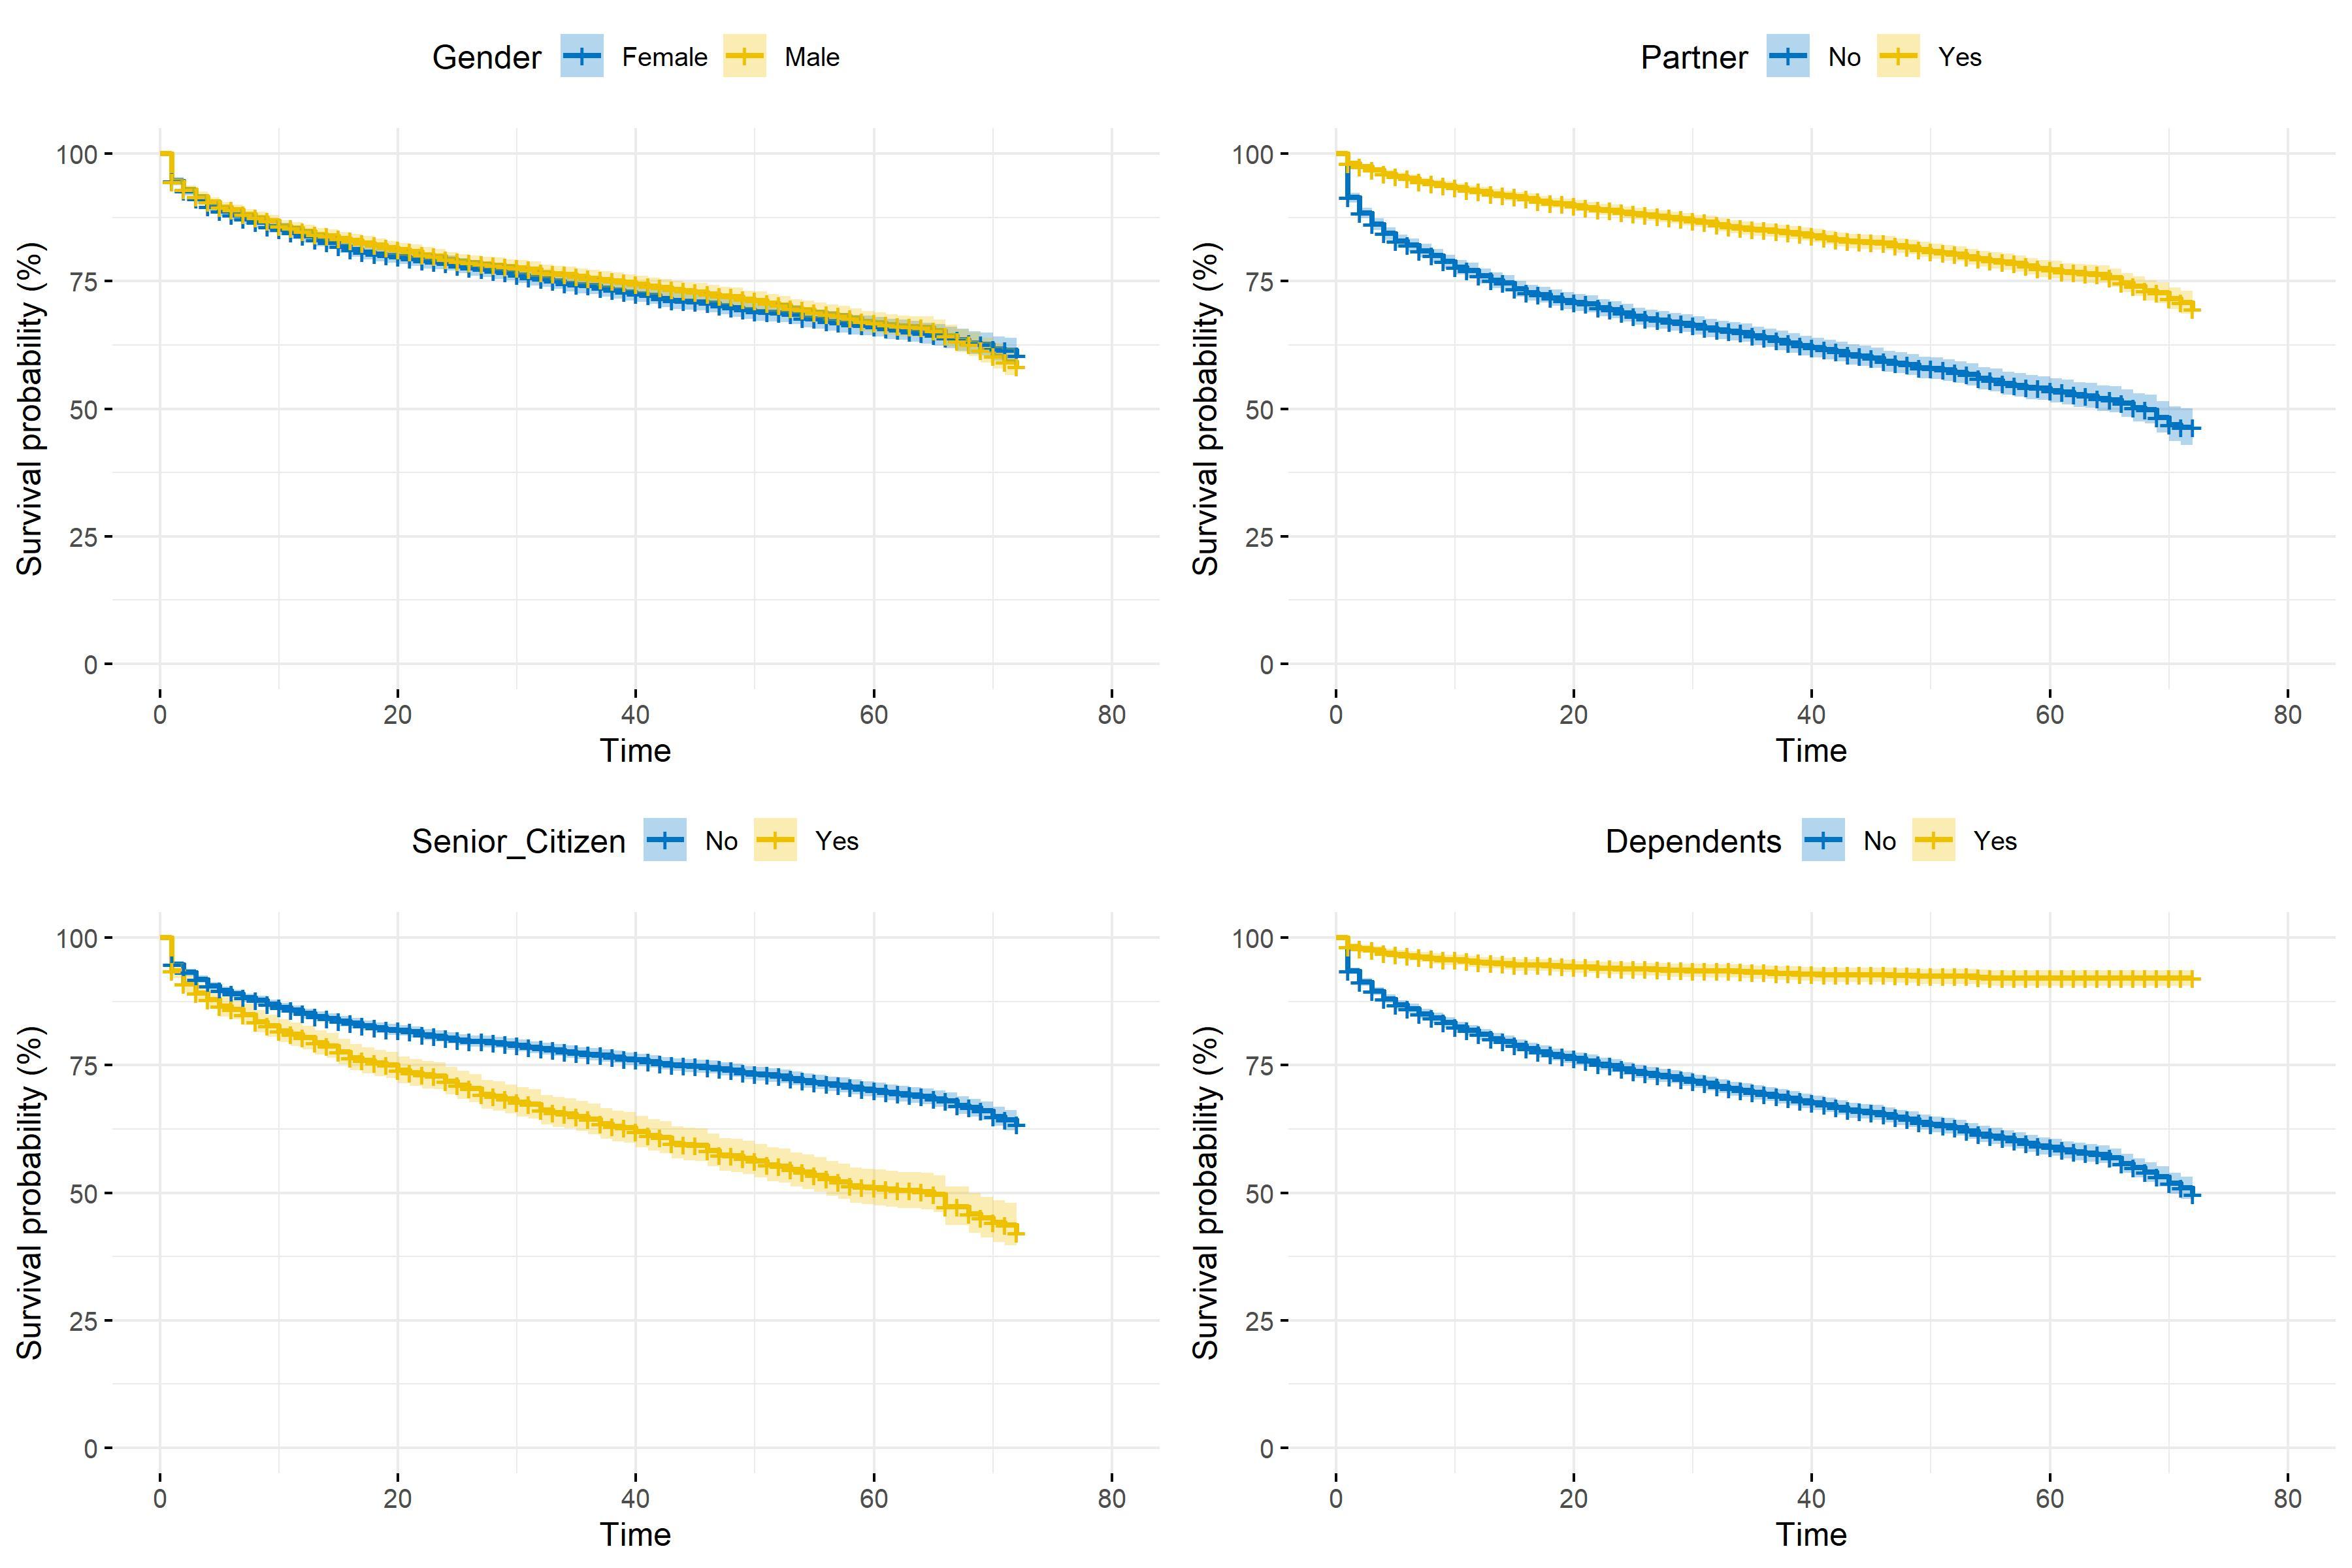
\includegraphics[width=50in]{./imgs/demographics_plot} 

}

\caption{Kaplan-Meier survival function depending on demographic information}\label{fig:kmdemographics}
\end{figure}

\hypertarget{data-on-services-subscribed}{%
\subsection*{Data on services subscribed}\label{data-on-services-subscribed}}
\addcontentsline{toc}{subsection}{Data on services subscribed}

When dealing with data on customers of a TSP, features related to services subscribed may be relevant to explain the estimated survival of these customers in the \emph{portfolio}.

Table \ref{tab:chi2services} presents results of \(\chi^2\) tests performed between \texttt{Churn\_Label} and each services information variable. As in the previous table, \emph{p-values} are ranked in ascending order. One can note that \texttt{Online\_Security} and \texttt{Tech\_Support} are the most linked to the churn indicator variable. However, variable carrying information on phone services are less correlated to \texttt{Churn\_Label}.

\begin{table}[H]

\caption{\label{tab:chi2services}Independence $\chi^2$ test between churn and services information variables}
\centering
\begin{tabular}[t]{lrrrl}
\toprule
  & Statistic & Df & Critical Value & p-value\\
\midrule
\cellcolor{gray!6}{Internet\_Service} & \cellcolor{gray!6}{728.70} & \cellcolor{gray!6}{2} & \cellcolor{gray!6}{5.99} & \cellcolor{gray!6}{5.8e-159}\\
Online\_Security & 205.42 & 1 & 3.84 & 1.4e-46\\
\cellcolor{gray!6}{Tech\_Support} & \cellcolor{gray!6}{189.97} & \cellcolor{gray!6}{1} & \cellcolor{gray!6}{3.84} & \cellcolor{gray!6}{3.2e-43}\\
Online\_Backup & 47.25 & 1 & 3.84 & 6.3e-12\\
\cellcolor{gray!6}{Device\_Protection} & \cellcolor{gray!6}{30.50} & \cellcolor{gray!6}{1} & \cellcolor{gray!6}{3.84} & \cellcolor{gray!6}{3.3e-08}\\
\addlinespace
Streaming\_TV & 27.84 & 1 & 3.84 & 1.3e-07\\
\cellcolor{gray!6}{Streaming\_Movies} & \cellcolor{gray!6}{25.76} & \cellcolor{gray!6}{1} & \cellcolor{gray!6}{3.84} & \cellcolor{gray!6}{3.9e-07}\\
Phone\_Service & 0.87 & 1 & 3.84 & 3.5e-01\\
\cellcolor{gray!6}{Multiple\_Lines} & \cellcolor{gray!6}{0.87} & \cellcolor{gray!6}{1} & \cellcolor{gray!6}{3.84} & \cellcolor{gray!6}{3.5e-01}\\
\bottomrule
\end{tabular}
\end{table}

Figure \ref{fig:kmservices} illustrates the \(\chi^2\) tests' results by representing the Kaplan-Meier estimated survivor function related to customer lifetime according to treatment variables on services subscribed. On the one hand, there seems to be no significant difference in terms of survival whether the customer uses phone service or not. The same remark can be pointed out based on whether the client has multiple lines as \texttt{Phone\_Service} and \texttt{Multiple\_Lines} might be quite correlated. In contrast, huge survival time difference can be noticed between customers with online security and those without, as well as between those having subscribed to technical support and those who have not. Finally, not using Internet service appears to have a positive influence on customer lifetime.

\begin{figure}

{\centering 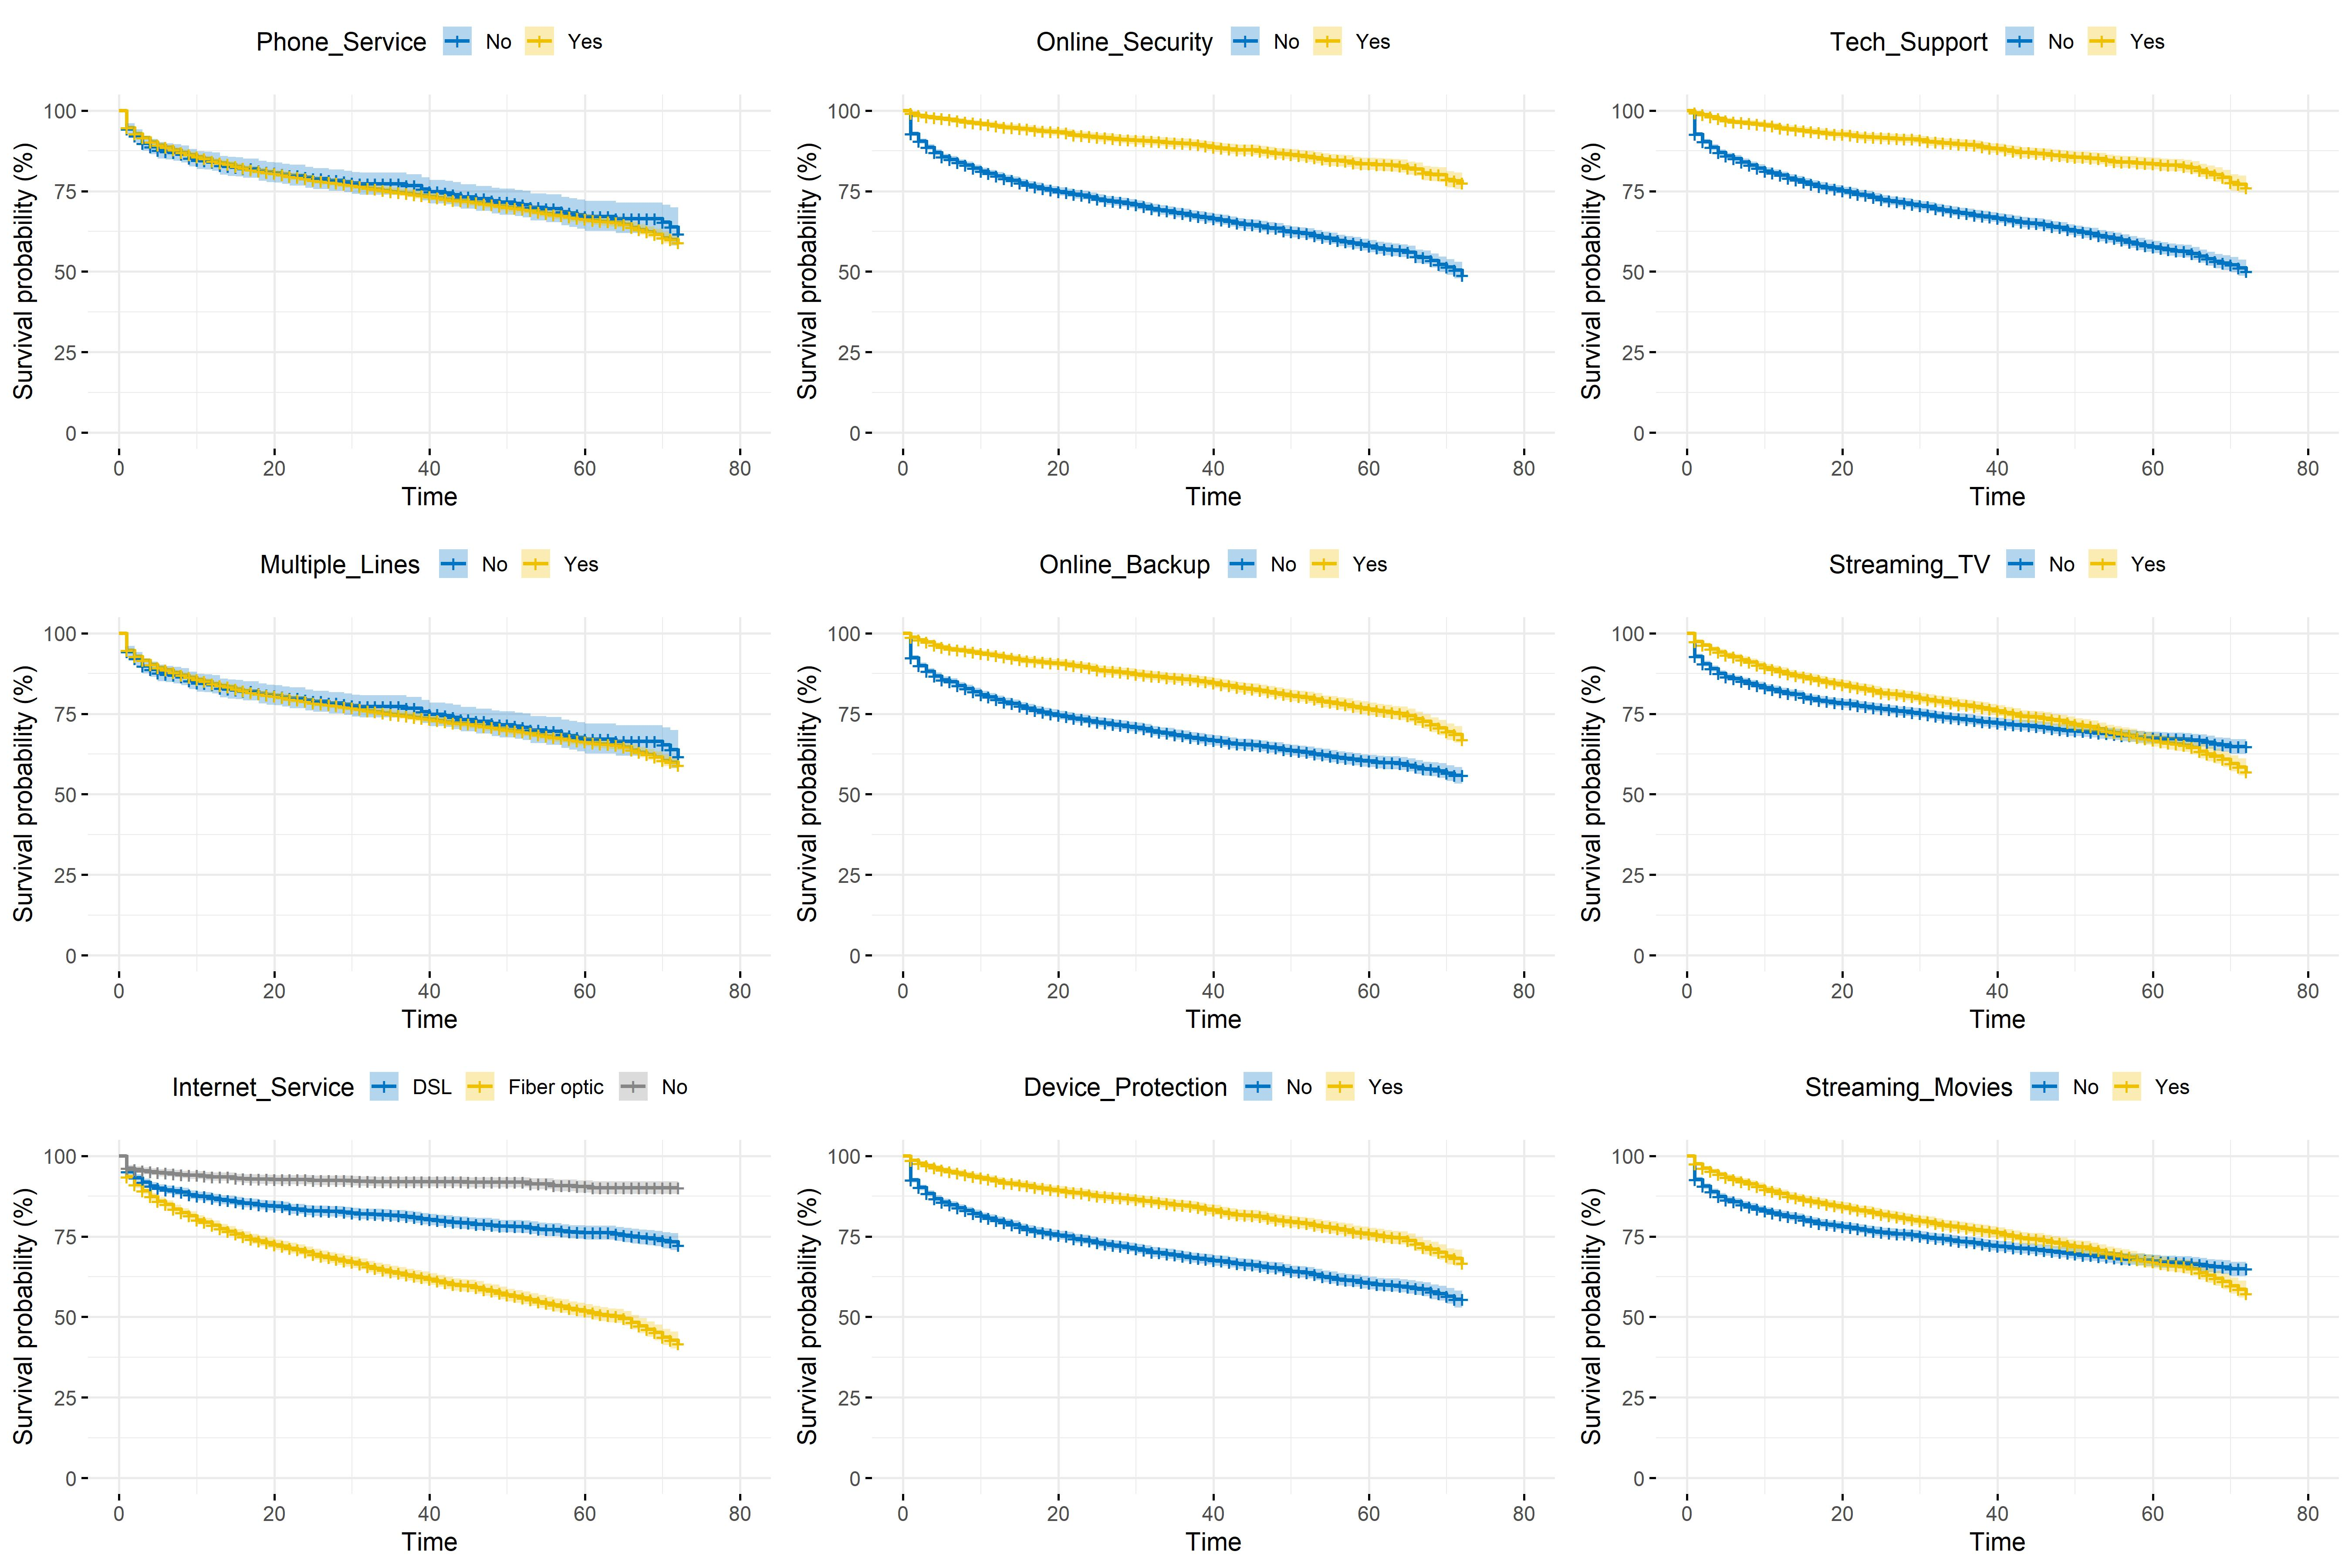
\includegraphics[width=75in]{./imgs/services_plot} 

}

\caption{Kaplan-Meier survival function depending on services subscribed}\label{fig:kmservices}
\end{figure}

\hypertarget{customer-account-data}{%
\subsection*{Customer account data}\label{customer-account-data}}
\addcontentsline{toc}{subsection}{Customer account data}

Variables on customer account such as the payment method used and the type of contract between the TSP and the client can be rich in information on customer lifetime. Indeed, table \ref{tab:chi2custaccount} shows that churn status strongly depends on the three variables, \texttt{Contract} being the most linked to \texttt{Churn\_Label}.

\begin{table}[H]

\caption{\label{tab:chi2custaccount}Independence $\chi^2$ test between churn and customer account data}
\centering
\begin{tabular}[t]{lrrrl}
\toprule
  & Statistic & Df & Critical Value & p-value\\
\midrule
\cellcolor{gray!6}{Contract} & \cellcolor{gray!6}{1179.55} & \cellcolor{gray!6}{2} & \cellcolor{gray!6}{5.99} & \cellcolor{gray!6}{7.3e-257}\\
Payment\_Method & 645.43 & 3 & 7.81 & 1.4e-139\\
\cellcolor{gray!6}{Paperless\_Billing} & \cellcolor{gray!6}{256.87} & \cellcolor{gray!6}{1} & \cellcolor{gray!6}{3.84} & \cellcolor{gray!6}{8.2e-58}\\
\bottomrule
\end{tabular}
\end{table}

Figure \ref{fig:kmcustaccount} enriches the \(\chi^2\) tests' results as it draws survival curves for each treatment variable's categories. When the firm/client contract is type month-to-month, the estimated survivor function decreases far more than for one-year or two-year contracts. In other words, the churn hazard is higher when the contract is renewed each month. This result makes sense as the customer may decide to leave the \emph{portfolio} once the month has ended as they are not commited for one or two years. Furthermore, clients with paperless billing contracts are more prone to churn, just like those paying by electronic check. It can be deduce that the \emph{attrition} risk is higher when the payment method is simplified.

\begin{figure}

{\centering 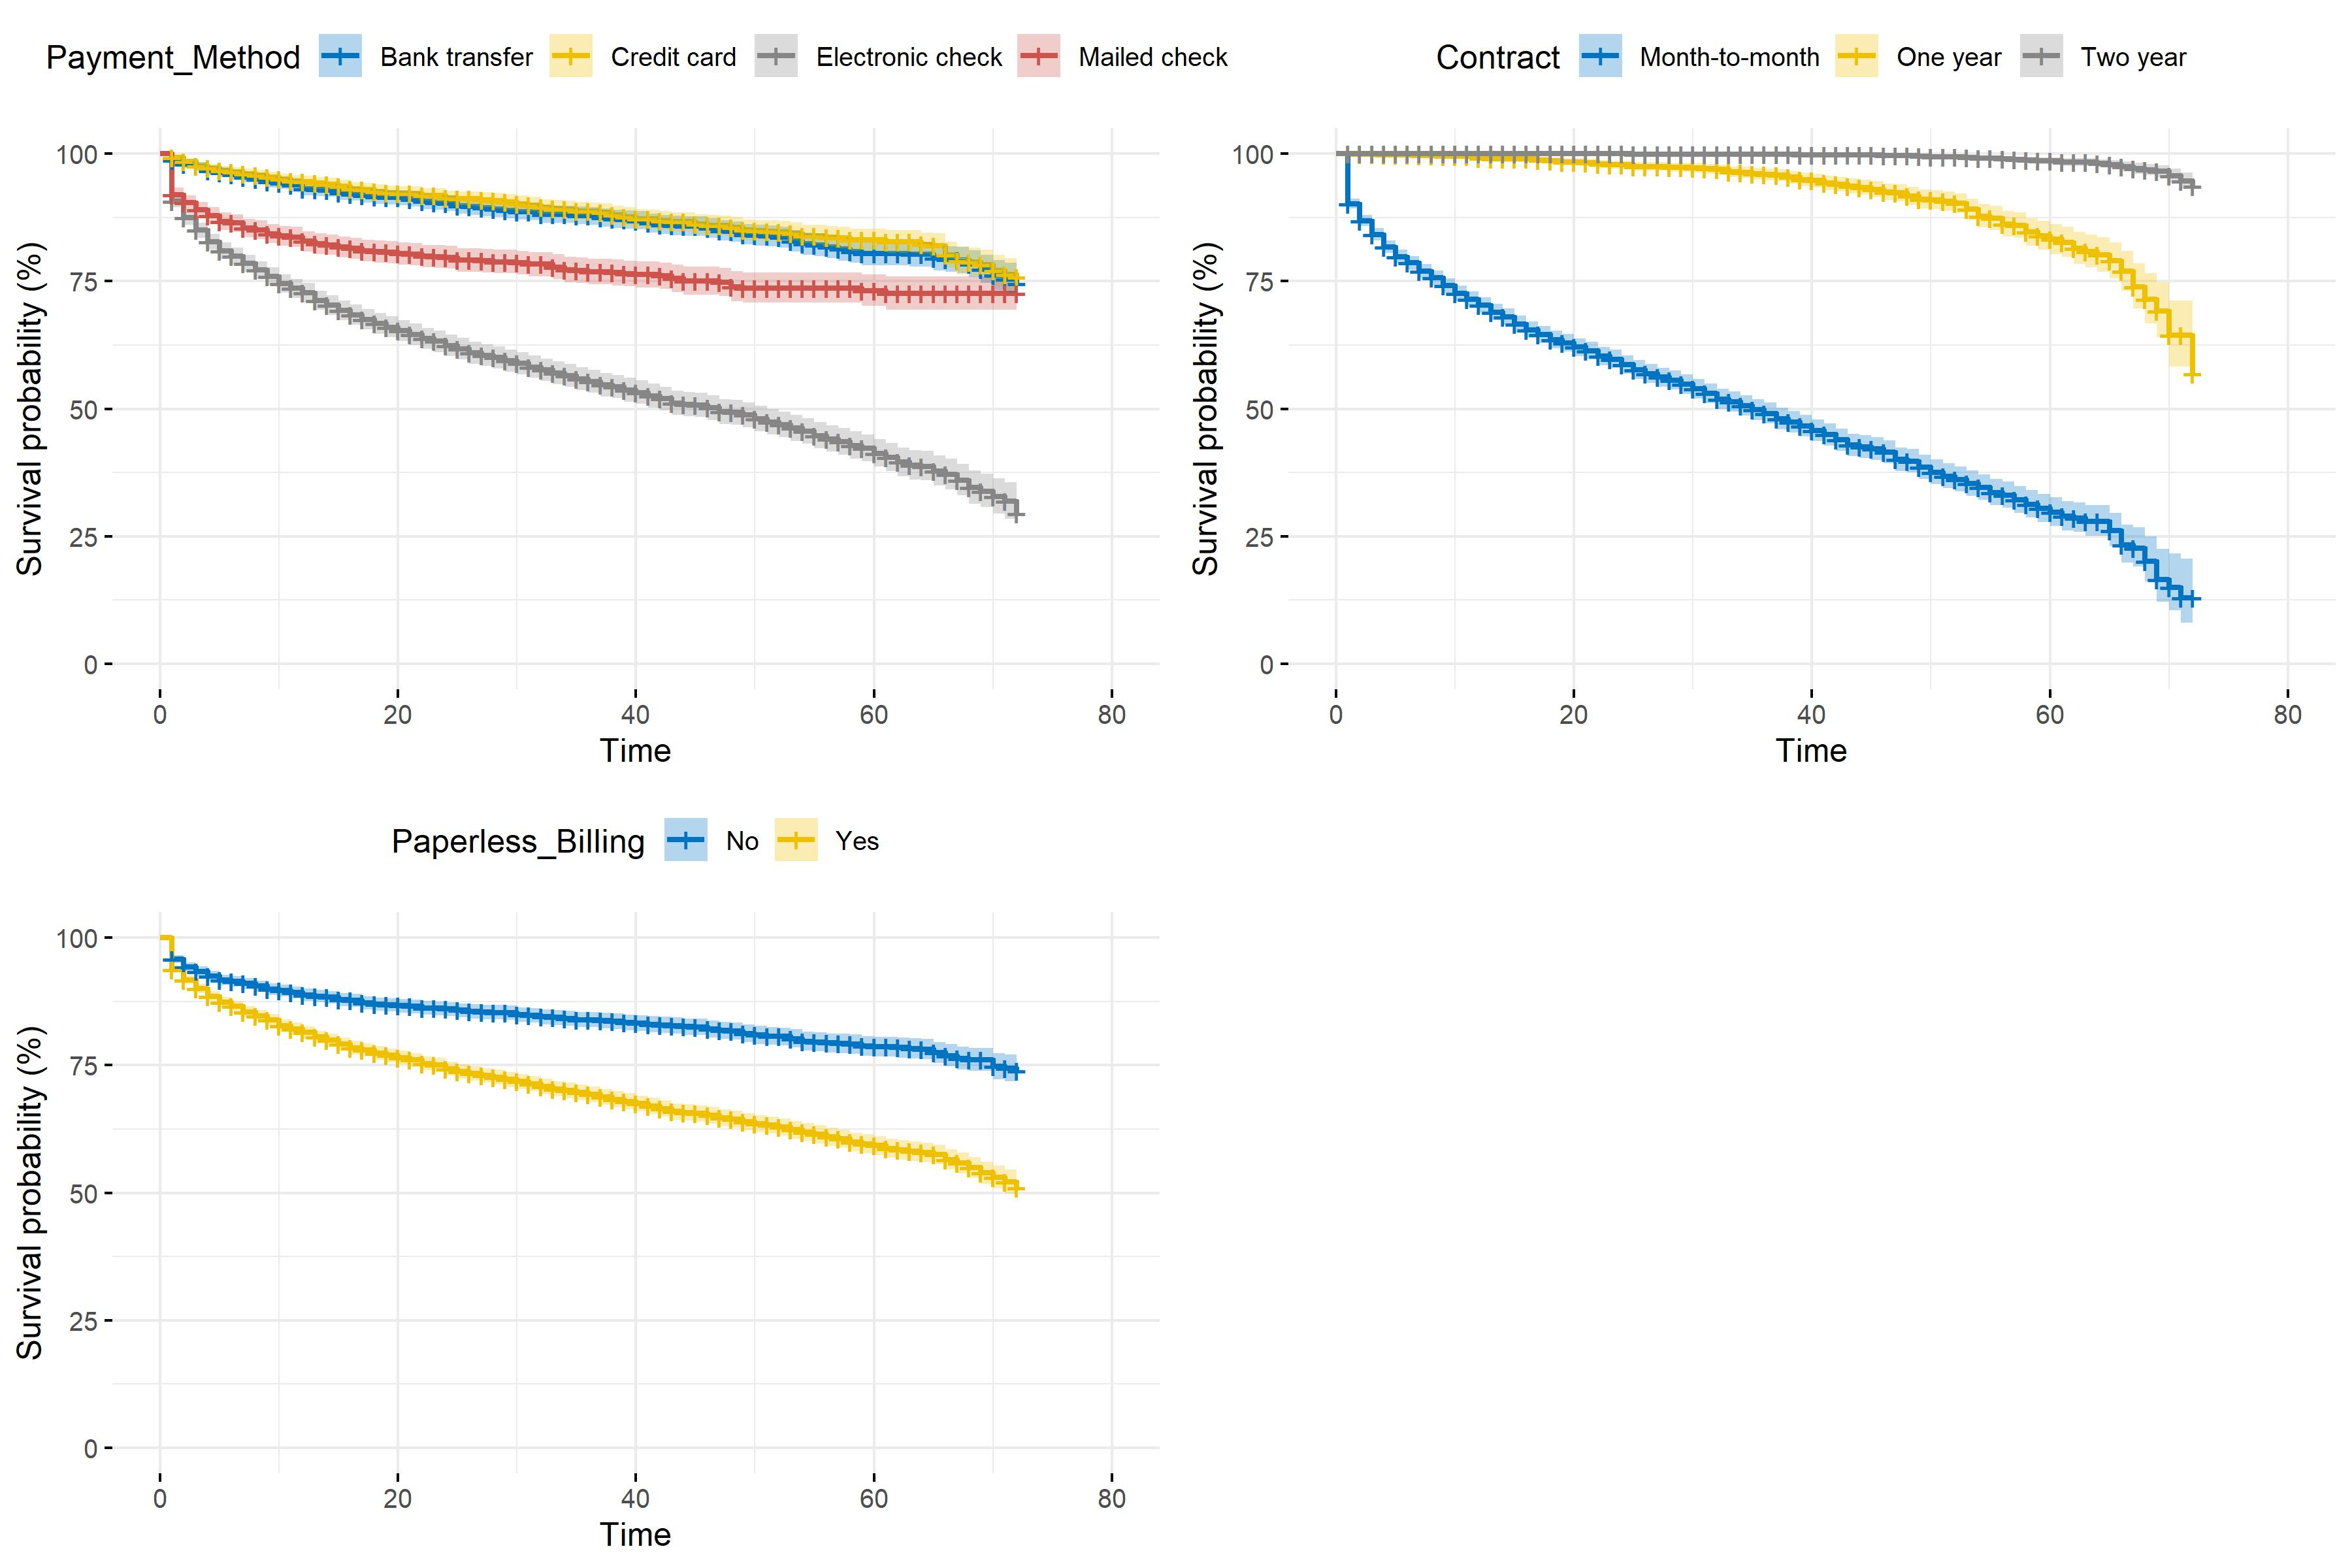
\includegraphics[width=50in]{./imgs/account_info_plot} 

}

\caption{Kaplan-Meier survival function depending on customer account information}\label{fig:kmcustaccount}
\end{figure}

\hypertarget{churn-duration-and-price}{%
\section{Churn, duration and price}\label{churn-duration-and-price}}

The final step in the data exploration consists in analysing the relationship between the \texttt{Monthly\_Charges}, \texttt{Churn\_Label} and \texttt{Tenure\_Months} variables as they play an important role in the modelling strategy we adopt to estimate customer \emph{value}.

Looking at figure \ref{fig:cltvchurn}, monthly charges seem to be higher for churners than for retained customers as the density is more right-oriented. High fees might be a driver of customer churn.

\begin{figure}

{\centering 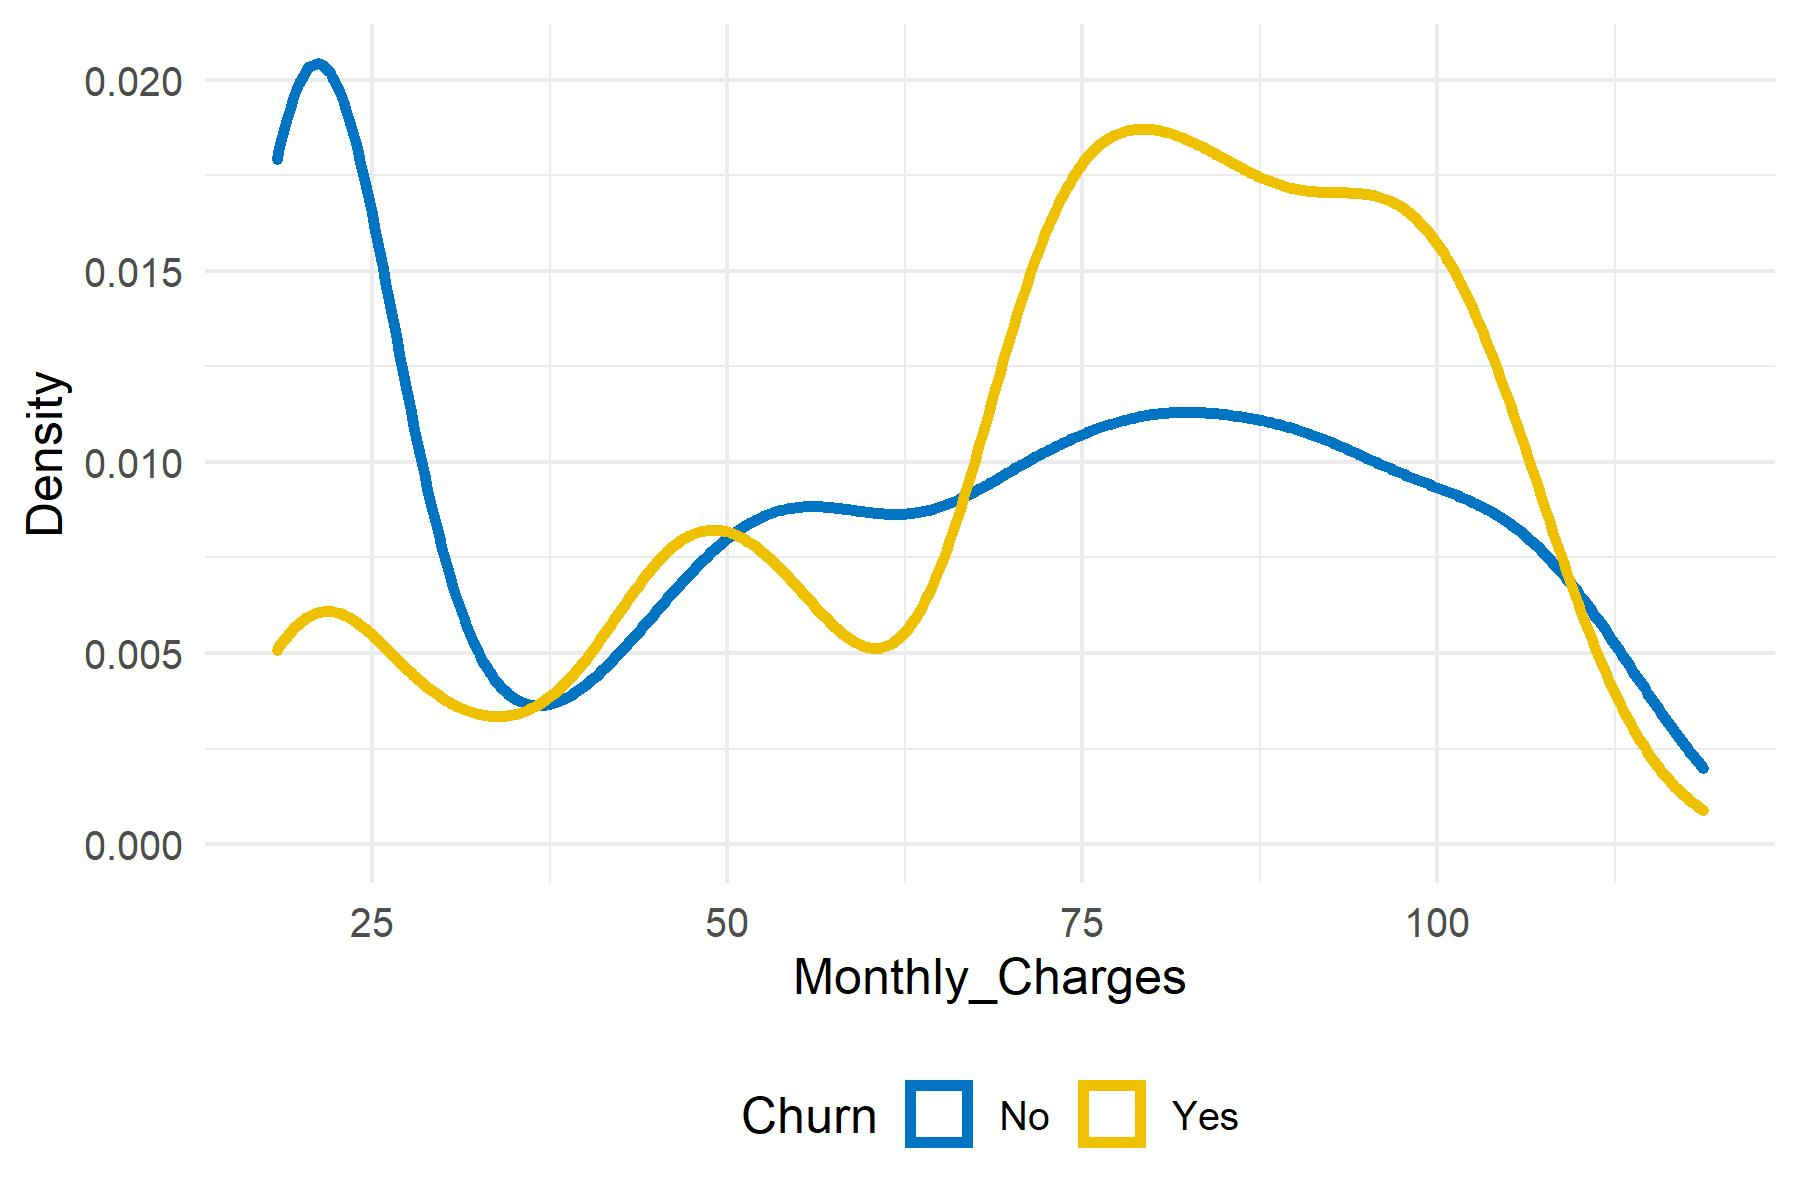
\includegraphics[width=400pt,height=300pt]{./imgs/monthly_charges_churn_plot} 

}

\caption{Monthly charges paid by customers depending on churn status}\label{fig:cltvchurn}
\end{figure}

Besides, the low \emph{p value} related to the Anova test between \texttt{CLTV} and \texttt{Churn\_Label} indicates that customer lifetime value is statistically different between churner and retained clients.

\begin{table}[H]

\caption{\label{tab:aovcltvchurn}Anova test between monthly fees and churn status}
\centering
\begin{tabular}[t]{lrrrl}
\toprule
  & F statistic & Df1 & Df2 & p-value\\
\midrule
\cellcolor{gray!6}{Churn\_Label} & \cellcolor{gray!6}{271.58} & \cellcolor{gray!6}{1} & \cellcolor{gray!6}{7030} & \cellcolor{gray!6}{6.8e-60}\\
\bottomrule
\end{tabular}
\end{table}

The following histograms are interesting to the extent that the distribution of \texttt{Tenure\_Months} depends on the churn status. From figure \ref{fig:churndur}, one can note an inflation of low and high values for retained customers. The distribution appears to be more homogeneous for retained clients than for churners. These lasts' tenure months distribution is decreasing and looks like a Poisson distribution with an inflation of low values.

\begin{figure}

{\centering 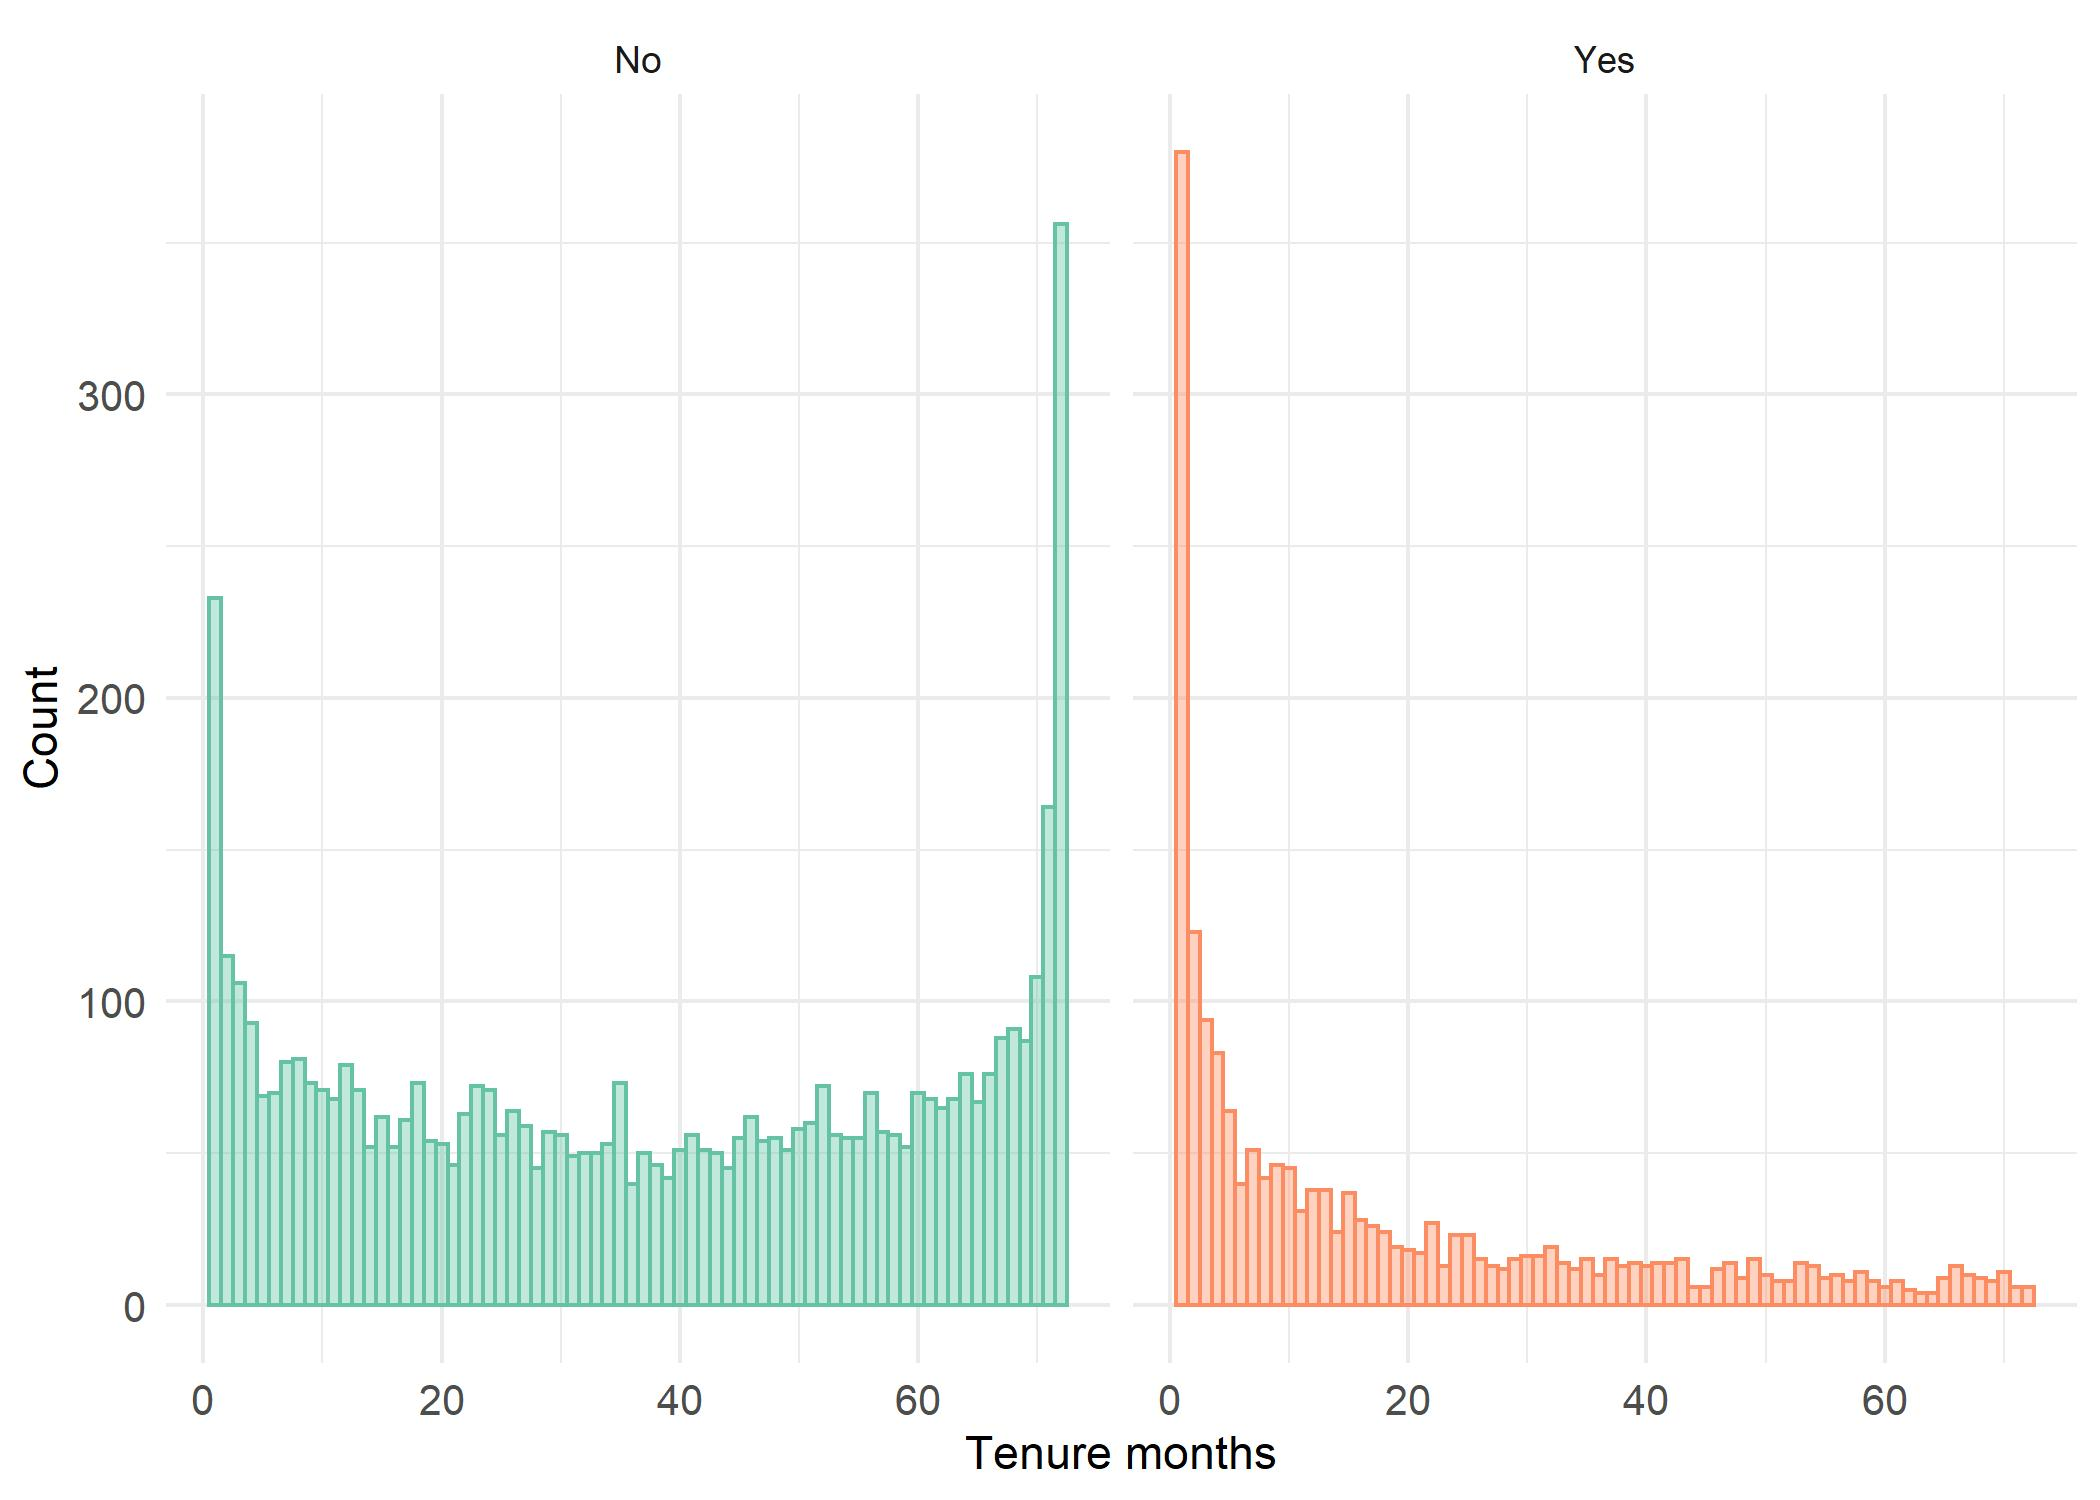
\includegraphics[width=500pt,height=350pt]{./imgs/duration_churn_plot} 

}

\caption{Tenure months depending on churn status}\label{fig:churndur}
\end{figure}

Eventually, figure \ref{fig:monthlychargesdur} depicts the average monthly charges per number of months in the portfolio. One can notice an increasing evolution between the average monthly fees and the number of months. In other words, it might be assumed that customers with longer lifetimes bring in more money to the firm.

\begin{figure}

{\centering 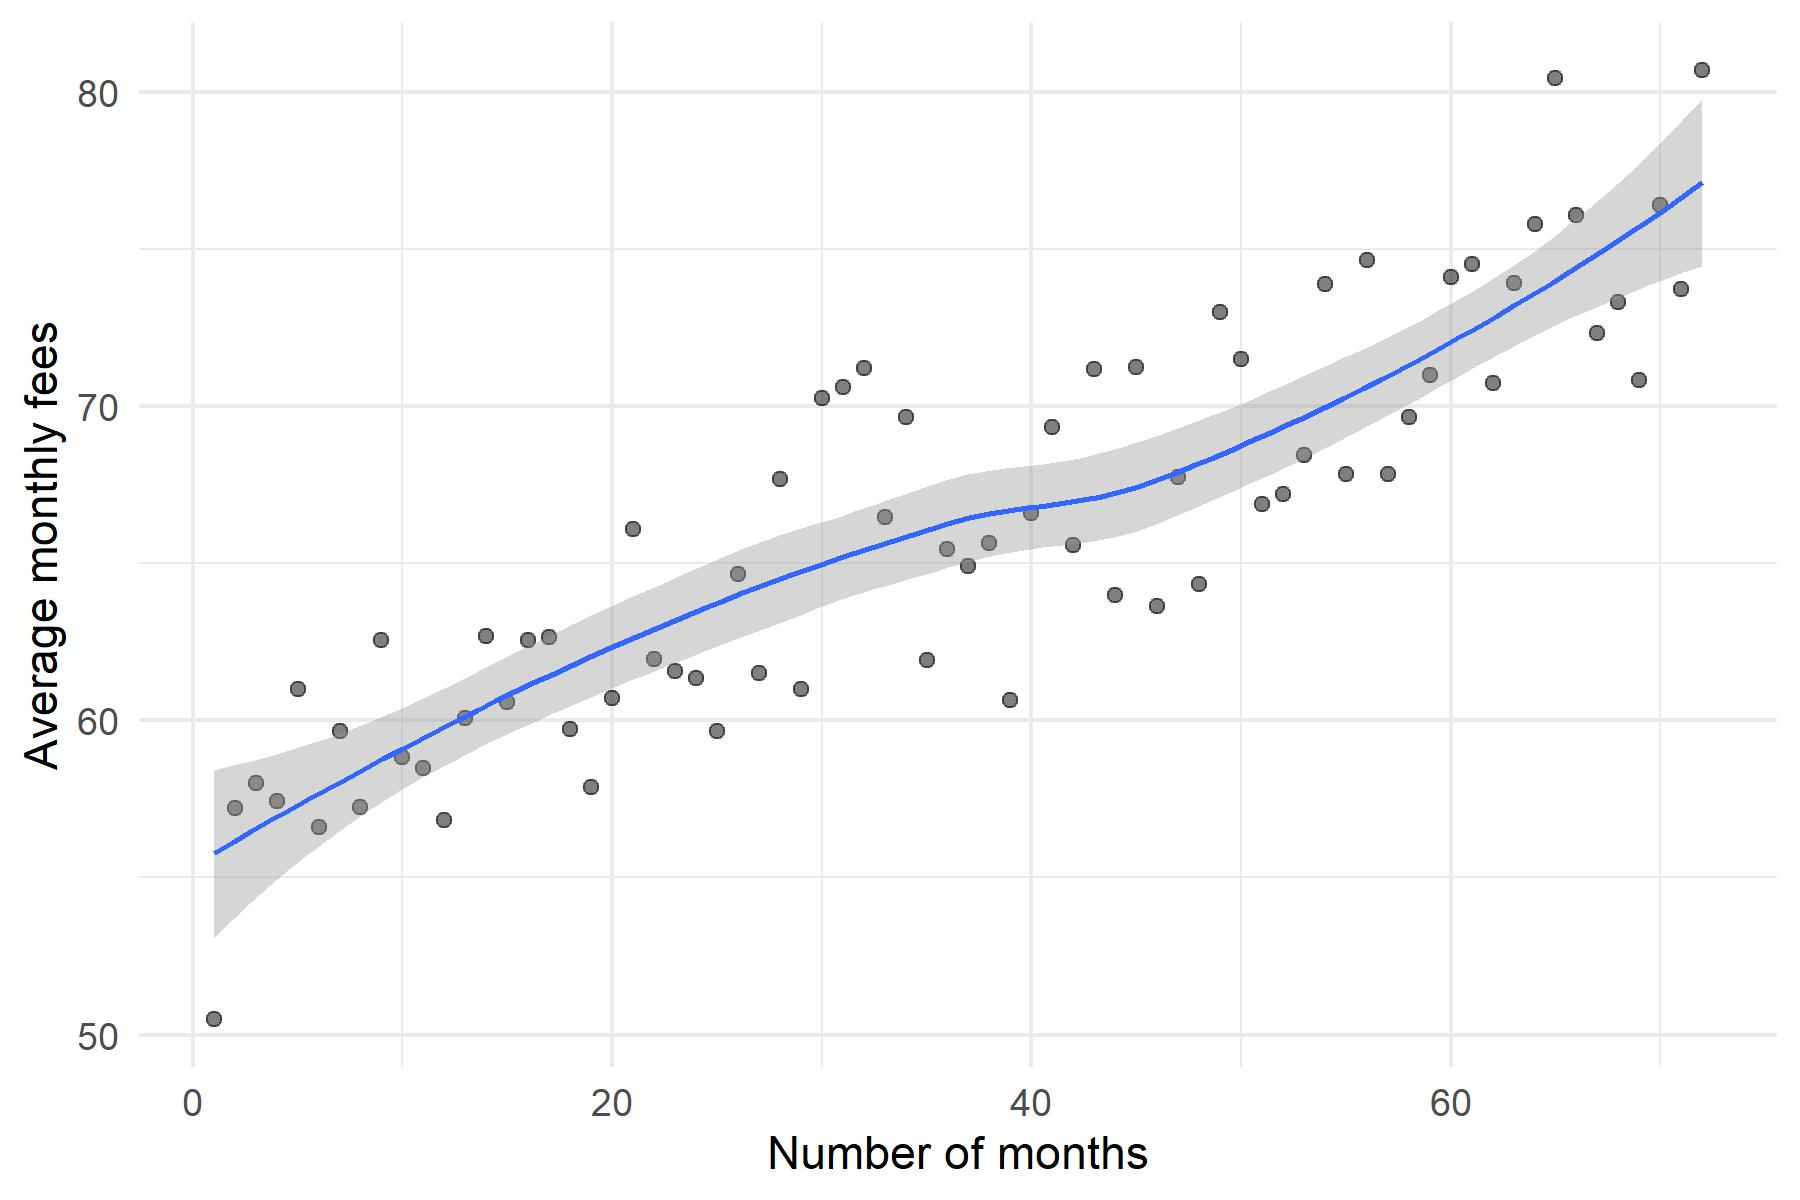
\includegraphics[width=450pt,height=300pt]{./imgs/monthly_charges_dur} 

}

\caption{Average monthly fees depending on number of months in the portfolio}\label{fig:monthlychargesdur}
\end{figure}

\hypertarget{estimation}{%
\chapter{Estimation techniques}\label{estimation}}

This chapter explains the different methods used to model a portfolio of customers as well as their related risk of attrition and the overall value of the portfolio. In a first part, clustering techniques are implemented to identify segments of customers based on services and account variables. Then, survival models are fitted to estimate each customer's survival in the firm's portfolio. The selected model can also be used to assess the effects of each variable on the risk of churn. Finally, we answer the study's problematic by computing an estimated value of the portfolio. The latter is calculated using a corporate formula and takes customers' monthly fees and survival probabilities as inputs. The estimated portfolio value is not cost-adjusted there is no information on consumers' costs in the data set.

\hypertarget{featureselection}{%
\section{Feature selection}\label{featureselection}}

Before fitting any survival model or clustering algorithm to the data, the initial step consists in selecting variables that are discriminating in terms of churn hazard. Based on Kaplan-Meier analysis depicted in section \ref{churndescstats}, we have a general overview of features which influence the survival probability. In other words, our feature selection method relies on results obtained with descriptive statistics.

Table \ref{tab:selectedfeatures} shows the selected variables for 5 random observations extracted from the data set. It can be noted that these features are related to account or service information, apart from \texttt{Dependents} which indicates whether the client lives with any dependents (children, parents, etc) and \texttt{Senior\_Citizen}. Furthermore, 9 out of the 10 selected variables are categorical which implies that the estimation results could be used to compare different groups of client. \texttt{Monthly\_Charges} is the only quantitative variable used to fit clustering models and survival regressions.

\begin{table}[H]

\caption{\label{tab:selectedfeatures}Explanatory variables used in survival models and cluster analysis}
\centering
\begin{tabular}[t]{lllllllllr}
\toprule
Senior\_Citizen & Dependents & Phone\_Service & Internet\_Service & Online\_Security & Online\_Backup & Tech\_Support & Contract & Payment\_Method & Monthly\_Charges\\
\midrule
\cellcolor{gray!6}{Yes} & \cellcolor{gray!6}{No} & \cellcolor{gray!6}{Yes} & \cellcolor{gray!6}{DSL} & \cellcolor{gray!6}{No} & \cellcolor{gray!6}{Yes} & \cellcolor{gray!6}{No} & \cellcolor{gray!6}{Month-to-month} & \cellcolor{gray!6}{Bank transfer} & \cellcolor{gray!6}{50.40}\\
No & Yes & Yes & No & No & No & No & Two year & Mailed check & 19.65\\
\cellcolor{gray!6}{No} & \cellcolor{gray!6}{Yes} & \cellcolor{gray!6}{Yes} & \cellcolor{gray!6}{Fiber optic} & \cellcolor{gray!6}{Yes} & \cellcolor{gray!6}{Yes} & \cellcolor{gray!6}{Yes} & \cellcolor{gray!6}{Two year} & \cellcolor{gray!6}{Credit card} & \cellcolor{gray!6}{114.30}\\
No & No & Yes & No & No & No & No & Month-to-month & Bank transfer & 19.95\\
\cellcolor{gray!6}{No} & \cellcolor{gray!6}{No} & \cellcolor{gray!6}{Yes} & \cellcolor{gray!6}{DSL} & \cellcolor{gray!6}{Yes} & \cellcolor{gray!6}{No} & \cellcolor{gray!6}{Yes} & \cellcolor{gray!6}{Month-to-month} & \cellcolor{gray!6}{Mailed check} & \cellcolor{gray!6}{54.45}\\
\bottomrule
\end{tabular}
\end{table}

\hypertarget{segmentation}{%
\section{Portfolio segmentation}\label{segmentation}}

Customer segmentation helps decision makers having a better understanding of their clients. It can then be used to enhance marketing strategies via personalization. In other words, segmentation can lead to target customers with offers and incentives personalized to their wants, needs and preferences. In order to make segmentation more accurate, it is more appropriate to use cluster analysis than predetermined thresholds or rules, even more when we have several variables at our disposal. In this context, this section focuses on applying clustering methods on features displayed in table \ref{tab:selectedfeatures}, apart from \texttt{Monthly\_Charges}.

\hypertarget{transforming-qualitative-variables-into-principal-axes}{%
\subsection{Transforming qualitative variables into principal axes}\label{transforming-qualitative-variables-into-principal-axes}}

The variables selected to perform cluster analysis being categorical, it is needed to transform them into continuous features. To that end, multiple correspondence analysis (MCA) is performed. MCA is a dimension reducing method which takes multiple categorical variables and seeks to identify associations between levels of those variables. MCA aims at highlighting features that separate classes of individuals, while determining links between variables and categories. To that end, MCA keeps the core information by the means of principal components which are projected axes \citep{MCA}.

Here, the main objective of applying MCA being to obtain continuous features, it is decided to keep as many axes as it takes to have at least 80\% cumulated variance. In other words, we want the principal components to gather enough customer-related information. After having processed the \texttt{MCA} function from the R package \texttt{FactoMineR} \citep{FactoMineR2008}, 10 principal components are required to keep more than 80\% cumulated variance as depicted by figure \ref{fig:mcascreeplot}.

\begin{figure}

{\centering 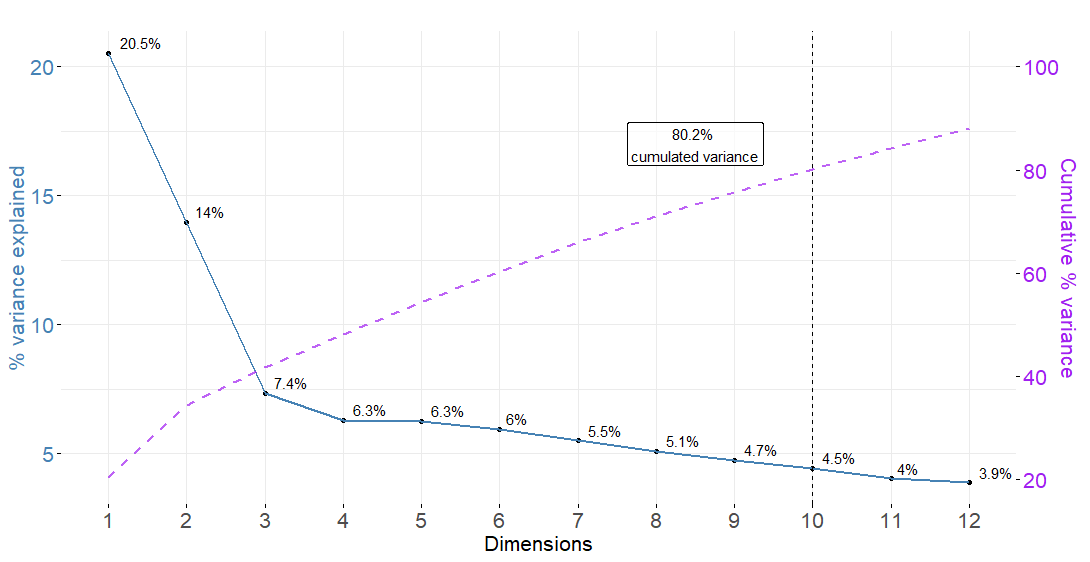
\includegraphics[width=15.14in]{./imgs/mca_screeplot} 

}

\caption{Variance explained and cumulated variance after MCA}\label{fig:mcascreeplot}
\end{figure}

Now the 10 continuous axes are identified, the next step consists in retrieving the customers' coordinates onto those axes to then perform cluster analysis.

\begin{table}[H]

\caption{\label{tab:unnamed-chunk-23}The 10 principal axes obtained by MCA}
\centering
\begin{tabular}[t]{rrrrrrrrrrr}
\toprule
CustomerID & Dim 1 & Dim 2 & Dim 3 & Dim 4 & Dim 5 & Dim 6 & Dim 7 & Dim 8 & Dim 9 & Dim 10\\
\midrule
\cellcolor{gray!6}{4197} & \cellcolor{gray!6}{-0.15} & \cellcolor{gray!6}{-0.02} & \cellcolor{gray!6}{-0.30} & \cellcolor{gray!6}{-0.03} & \cellcolor{gray!6}{0.03} & \cellcolor{gray!6}{-0.29} & \cellcolor{gray!6}{-0.61} & \cellcolor{gray!6}{0.01} & \cellcolor{gray!6}{-0.04} & \cellcolor{gray!6}{0.10}\\
3025 & 0.53 & 0.04 & 0.08 & 0.26 & 0.09 & -0.54 & 0.55 & 0.40 & -0.02 & -0.19\\
\cellcolor{gray!6}{6585} & \cellcolor{gray!6}{-0.04} & \cellcolor{gray!6}{-0.24} & \cellcolor{gray!6}{-0.15} & \cellcolor{gray!6}{0.40} & \cellcolor{gray!6}{0.07} & \cellcolor{gray!6}{-0.20} & \cellcolor{gray!6}{0.18} & \cellcolor{gray!6}{-0.25} & \cellcolor{gray!6}{0.02} & \cellcolor{gray!6}{0.07}\\
3862 & -0.44 & -0.20 & -0.46 & -0.14 & -0.01 & 0.01 & -0.05 & -0.04 & -0.52 & 0.01\\
\cellcolor{gray!6}{300} & \cellcolor{gray!6}{0.21} & \cellcolor{gray!6}{-0.37} & \cellcolor{gray!6}{0.11} & \cellcolor{gray!6}{0.00} & \cellcolor{gray!6}{0.00} & \cellcolor{gray!6}{-0.41} & \cellcolor{gray!6}{-0.54} & \cellcolor{gray!6}{-0.13} & \cellcolor{gray!6}{0.36} & \cellcolor{gray!6}{0.06}\\
\bottomrule
\end{tabular}
\end{table}

Note that a more in-depth visualisation of those 10 principal components can be found in figures \ref{fig:mcacontrib12} to \ref{fig:mcacontrib910} in the appendix. This charts depict the percent contribution of each variable's categories to the principal axes, which is helpful to have a better understanding of MCA results.

\hypertarget{hierarchical-clustering-on-principal-components}{%
\subsection{Hierarchical clustering on principal components}\label{hierarchical-clustering-on-principal-components}}

Multiple correspondence analysis has led us to convert the categorical variables related to account and services information into 10 numerical projected axes. The stake here is to use the customers' projections onto the MCA components in order to identify groups of individuals through clustering techniques. As a reminder, clusters are expected to discriminate between customers based on the services they use and the type of plan they are enrolled into. The method implemented in this part relies on hierarchical clustering on principal components (HCPC).

\hypertarget{optimal-number-of-clusters}{%
\subsubsection*{Optimal number of clusters}\label{optimal-number-of-clusters}}
\addcontentsline{toc}{subsubsection}{Optimal number of clusters}

The key parameter to optimize when applying clustering methods is the number of clusters \(k\). When using the \texttt{HCPC} function from \texttt{FactorMineR}, the \texttt{nb.clust} parameter is set to -1 so that the tree is automatically cut at the suggested level. More precisely, the function first builds a hierarchical tree. Then the sum of the between-cluster inertia is calculated for each partition. The suggested partition is the one with the higher relative gain in inertia. Intuitively, the underlying objective is to choose a number of clusters leading to \(k\) well distinguished groups. Here, the between-cluster inertia is the metric measuring the amount of variability between clusters.

\begin{figure}

{\centering 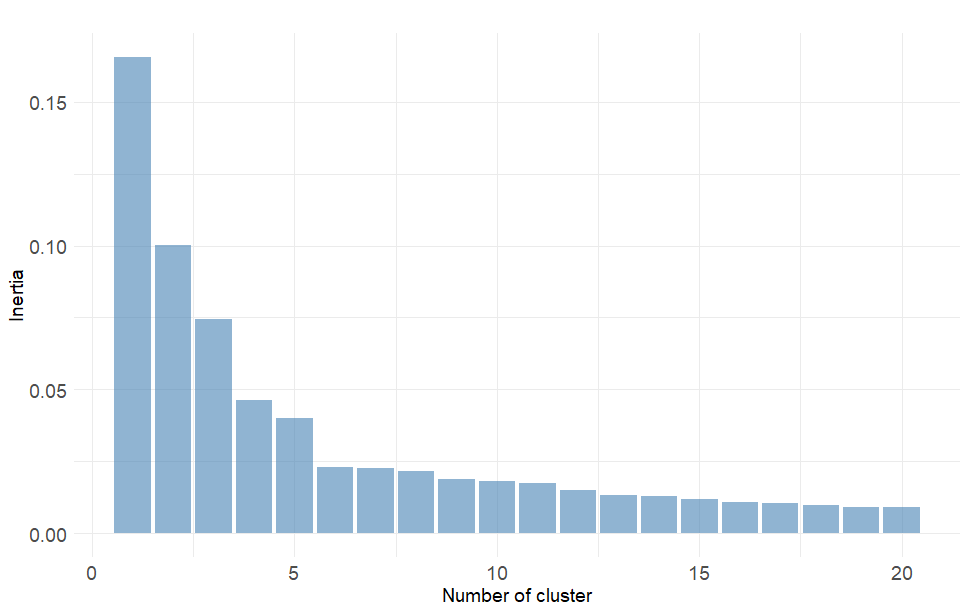
\includegraphics[width=13.89in]{./imgs/btw_inertia} 

}

\caption{Relative gains in between-cluster inertia given the partition}\label{fig:btwinertia}
\end{figure}

Once the 3 groups identified by the clustering algorithm, one can determine customer repartition within those groups. Looking at table \ref{tab:clustRepartition}, cluster 2 represents the largest share of clients. This result is illustrated on figure \ref{fig:clusterplot}.

\begin{table}[H]

\caption{\label{tab:clustRepartition}Customer repartition within the 3 clusters}
\centering
\begin{tabular}[t]{lrrr}
\toprule
  & Cluster 1 & Cluster 2 & Cluster 3\\
\midrule
\cellcolor{gray!6}{\%} & \cellcolor{gray!6}{26.55} & \cellcolor{gray!6}{41.38} & \cellcolor{gray!6}{32.07}\\
\bottomrule
\end{tabular}
\end{table}

\hypertarget{cluster-visualisation}{%
\subsubsection*{Cluster visualisation}\label{cluster-visualisation}}
\addcontentsline{toc}{subsubsection}{Cluster visualisation}

When performing hierarchical clustering on principal components, visualizing cluster repartition onto MCA axes is relevant to have a first idea on how each cluster if different from the others. Figure \ref{fig:clusterplot} indicates that the three clusters are well separated in the \((F_1 ; F_2)\) plan. Cluster 1 is more concentrated than the others and take lower values onto dimension 1. The second group spreads over axis 1 and takes lower values on axis 2. Finally, cluster 3's position shows that its customers are characterized by categories which take positive values on both dimensions 1 and 2.

\begin{figure}

{\centering 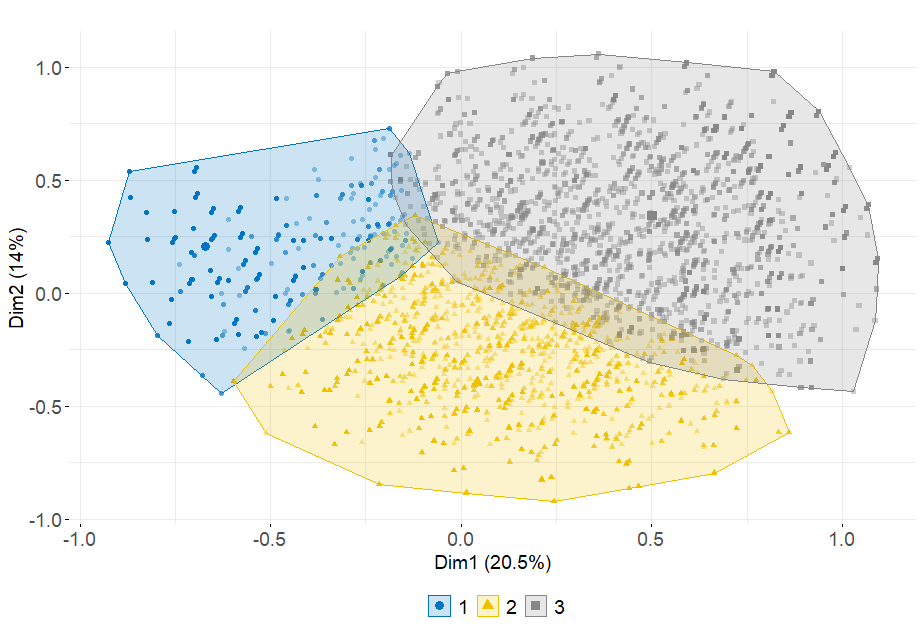
\includegraphics[width=12.83in]{./imgs/cluster_plot} 

}

\caption{Cluster visualisation onto the 2 first MCA axes}\label{fig:clusterplot}
\end{figure}

In the appendix, figure \ref{fig:clusterplots} aims at visualizing clusters onto the other MCA principal components. Note that none of theses axes manages to separate the three clusters. This may be due to the low amount of variance each of these axes carries.

\hypertarget{cluster-description}{%
\subsubsection*{Cluster description}\label{cluster-description}}
\addcontentsline{toc}{subsubsection}{Cluster description}

Once the 3 customer segments are identified on the MCA dimensions, it seems to be interesting to describe them according to the original features. To that end, the repartition of qualitative variables' categories is depicted on the following figure. Comparing figures \ref{fig:clusterplot} and \ref{fig:mcaplot}, one can derive the following table in order to have a more precise idea on each segment.

\begin{table}[H]

\caption{\label{tab:unnamed-chunk-24}The most representative categories for each cluster}
\centering
\begin{tabular}[t]{rl}
\toprule
Cluster & Representative Categories\\
\midrule
\cellcolor{gray!6}{1} & \cellcolor{gray!6}{Mailed\_check, Internet\_Service\_No}\\
2 & Month-to-month, Electronic check, Tech\_Support\_No\\
\cellcolor{gray!6}{3} & \cellcolor{gray!6}{Two year, Credit card, Tech\_Support\_Yes}\\
\bottomrule
\end{tabular}
\end{table}

The first segment may be made up of customers having subscribed to minimum plans whith no internet service whereas segment 3 tends to represent clients with a large variety of services and long-term contracts. On the opposite, cluster 2 clients are enrolled in short-term plans with internet service but not technical options.

\begin{figure}

{\centering 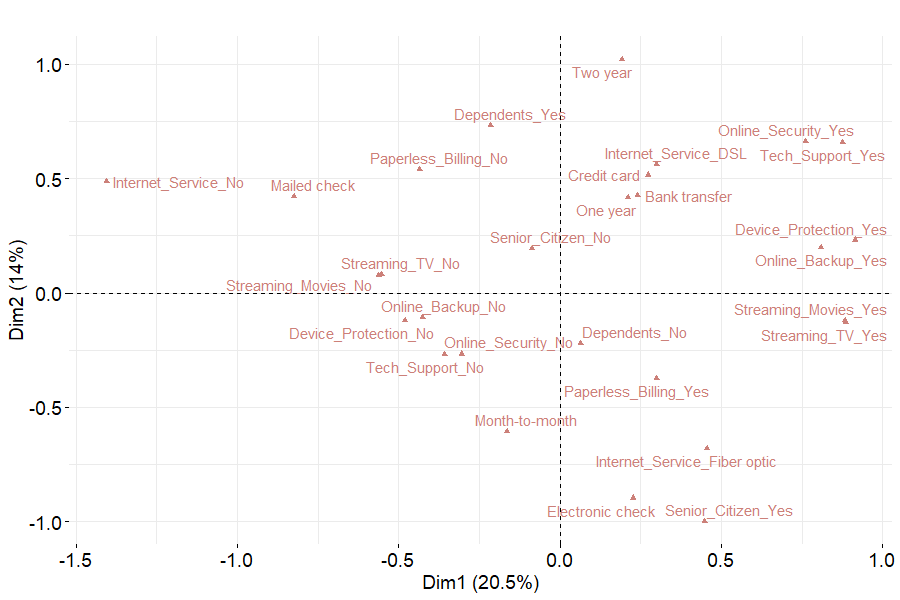
\includegraphics[width=12.5in]{./imgs/mca_plots} 

}

\caption{MCA - Categories plot onto the two first axes}\label{fig:mcaplot}
\end{figure}

Figure \ref{fig:monthlychargesclust} depicts the differences in monthly charges paid by each customer segment. It can be observed that most of cluster 1 clients are enrolled in cheap subscriptions. On the contrary, the charges paid by the second and third clusters are higher and less homogeneous. Note that the median price is the same among these two groups.

\begin{figure}

{\centering 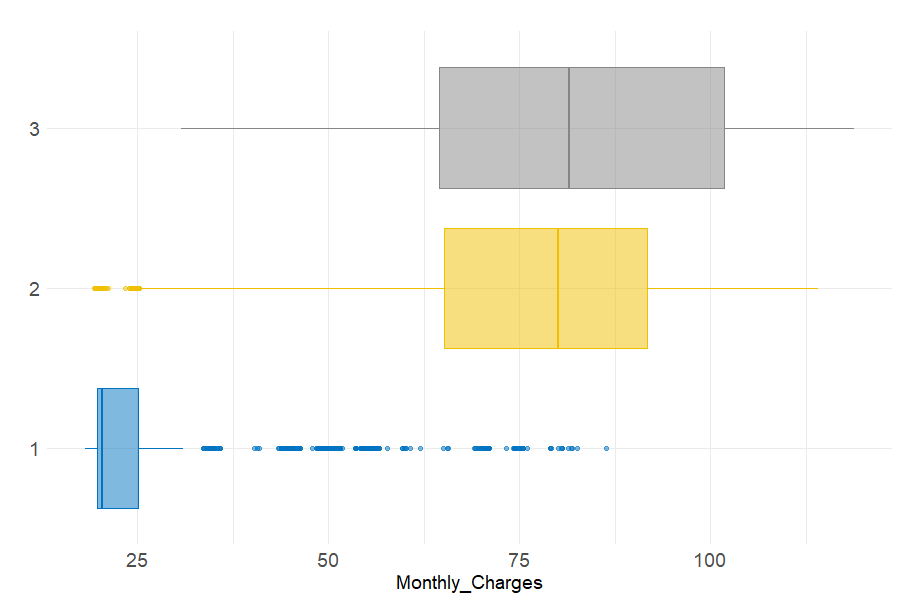
\includegraphics[width=0.7\linewidth,height=0.6\textheight]{./imgs/monthly_charges_clust} 

}

\caption{Monthly charges repartition across clusters}\label{fig:monthlychargesclust}
\end{figure}

Since one of the study's purpose is to model customer churn, it is important to compare the churn rate across the 3 groups. Here, the striking point is that cluster 2 clients account for a large proportion of churners. Indeed, more than 75\% of the clients having left the portfolio come from the second group. It can also be noted that cluster 1 and 3 are composed of more loyal customers as more than 70\% of clients who did not churn are from those 2 groups.

\begin{figure}

{\centering 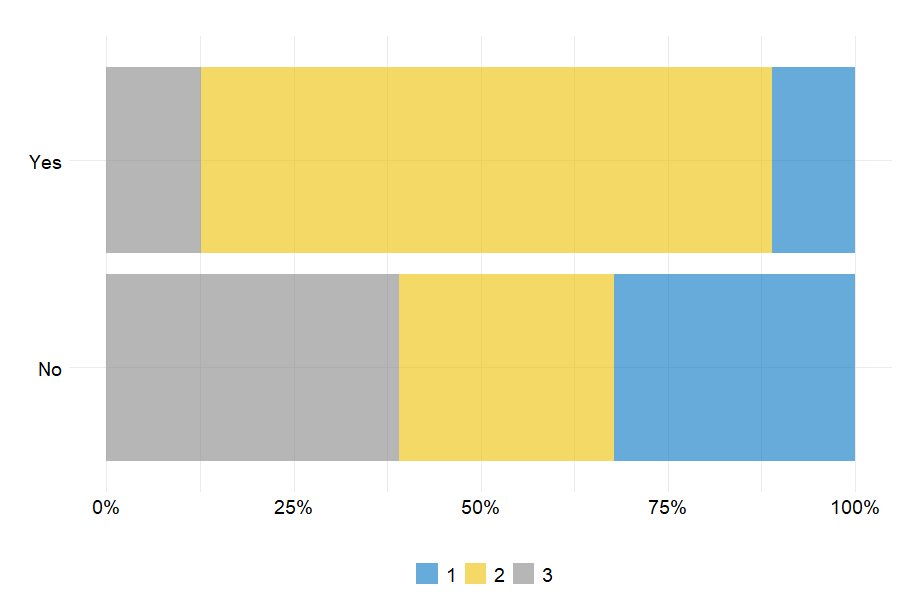
\includegraphics[width=0.6\linewidth,height=0.6\textheight]{./imgs/churn_cluster_barplot} 

}

\caption{Churn repartition per cluster}\label{fig:catvarsclust}
\end{figure}

\hypertarget{concluding-remarks-on-portfolio-segmentation}{%
\subsubsection*{Concluding remarks on portfolio segmentation}\label{concluding-remarks-on-portfolio-segmentation}}
\addcontentsline{toc}{subsubsection}{Concluding remarks on portfolio segmentation}

With the aim of divide the portfolio into multiple groups based on categorical features, hierarchical clustering on principal components has led to identify three customer segments which can be broadly described as shown in the following table.

\begin{table}[H]

\caption{\label{tab:unnamed-chunk-25}Portfolio segmentation summary}
\centering
\begin{tabular}[t]{rll>{}l}
\toprule
Cluster & Loyalty & Value & Segment name\\
\midrule
\cellcolor{gray!6}{1} & \cellcolor{gray!6}{High} & \cellcolor{gray!6}{Low} & \em{\cellcolor{gray!6}{Silver}}\\
\textbf{2} & \textbf{Low} & \textbf{High} & \textbf{\em{Gold}}\\
\cellcolor{gray!6}{3} & \cellcolor{gray!6}{High} & \cellcolor{gray!6}{High} & \em{\cellcolor{gray!6}{Platinum}}\\
\bottomrule
\end{tabular}
\end{table}

\emph{Gold} customers are valuable to the firm but are not loyal, making them the target segment. The objective would be to encourage them to stay in the portfolio longer.

\hypertarget{churnAnalysis}{%
\section{Churn analysis}\label{churnAnalysis}}

Estimating the risk of attrition related to each customer is an essential step to model the firm's portfolio. In this context, survival models can be implemented with a view of deriving a predicted churn risk and survival function for each client. One the one hand, these predictions can be used to identify loyal consumers and make appropriate decisions. For instance, it might be relevant to offer benefits to a high-value client with a high estimated churn risk. On the other hand, a customer's survival probability at time \(t\) represents the chance that this very customer be active in the portfolio at time \(t\). This measure is helpful to compute the estimated value of the portfolio in the last section.

Before presenting the estimation results, it seems important to recall that \texttt{Tenure\_Months} and \texttt{Churn\_Value} can be seen as a pair of time and event variables used as target in survival models.

\begin{table}[H]

\caption{\label{tab:survtarget}Time and event variables for survival models}
\centering
\begin{tabular}[t]{rrr}
\toprule
CustomerID & Tenure\_Months & Churn\_Value\\
\midrule
\cellcolor{gray!6}{1671} & \cellcolor{gray!6}{30} & \cellcolor{gray!6}{1}\\
6705 & 43 & 0\\
\cellcolor{gray!6}{3702} & \cellcolor{gray!6}{12} & \cellcolor{gray!6}{0}\\
1519 & 1 & 1\\
\cellcolor{gray!6}{4882} & \cellcolor{gray!6}{50} & \cellcolor{gray!6}{0}\\
\bottomrule
\end{tabular}
\end{table}

\hypertarget{coxmodel}{%
\subsection{The Cox model}\label{coxmodel}}

When it comes to choose an estimation method on survival data, the Cox PH model appears to be an interesting first choice. As explained in chapter \ref{duration}, this semi-parametric model makes no assumption regarding the nature of the baseline hazard function \(\lambda_0(t)\). The parametric part only relies in the modelling of the effect of some covariates on the hazard function \(\lambda(t)\) (see section \ref{coxph} for more details).

\hypertarget{fitting-the-model-on-the-selected-features}{%
\subsubsection*{Fitting the model on the selected features}\label{fitting-the-model-on-the-selected-features}}
\addcontentsline{toc}{subsubsection}{Fitting the model on the selected features}

Using the \texttt{coxph} function from the \texttt{survival} R library \citep{survival-book}, we are able to train a Cox model on the feature vector identified in section \ref{featureselection}. Once the model fitted, it seems relevant to evaluate its performance on the train data set. Table \ref{tab:lrtest} compares the model's log-likelihood to the constrained model's. Given the very low p-value, it can be assumed that the Cox model better fits the data than a model with only the intercept.

\begin{table}[H]

\caption{\label{tab:lrtest}Log-likelihood ratio test}
\centering
\begin{tabular}[t]{lrrr}
\toprule
  & Model & Constrained & pvalue\\
\midrule
\cellcolor{gray!6}{} & \cellcolor{gray!6}{-9228.77} & \cellcolor{gray!6}{-10448.08} & \cellcolor{gray!6}{0}\\
\bottomrule
\end{tabular}
\end{table}

Concordance index \(c\) is another metric to assess the performance of models which produces risk scores and is defined as the probability to well predict the order of event occurring time for any pair of instances. For the Cox model, the C-index obtained on the training set is \(c \approx 0.865 \pm 0.004\), which is more than satisfying.

\hypertarget{marginal-effects-1}{%
\subsubsection*{Marginal effects}\label{marginal-effects-1}}
\addcontentsline{toc}{subsubsection}{Marginal effects}

In the Cox model, the relative hazard between two observations is assumed to be constant over time. As a consequence, the relative hazard becomes \(\exp \hat{\beta}\) for both dummy and continuous variables. For instance regarding figure \ref{fig:coxmarginaleffects}, the relative hazard ratio between customers with a two-year contract and those with a month-to-month contract is 0.046, meaning that the latter group is 22 times more prone to churn than the former. Also, month-to-month clients are about 5 times more likely to churn than customers enrolled in one-year plan. When analysing the relative hazard ratios related to the payment method, it comes that clients who pay by electronic or mailed check are two times riskier to churn than those who pay by bank transfer. Furthermore, being enrolled in a plan with additional services like \texttt{Online\_Security}, \texttt{Online\_Backup} or \texttt{Tech\_Support} tends to decrease the estimated churn risk. As for the effect of the \texttt{Internet\_Service} covariate on the risk of attrition, it seems to be mitigated since clients who have a fiber optic internet connection are more than twice as likely to churn as those using a DSL internet connection.

\begin{figure}

{\centering 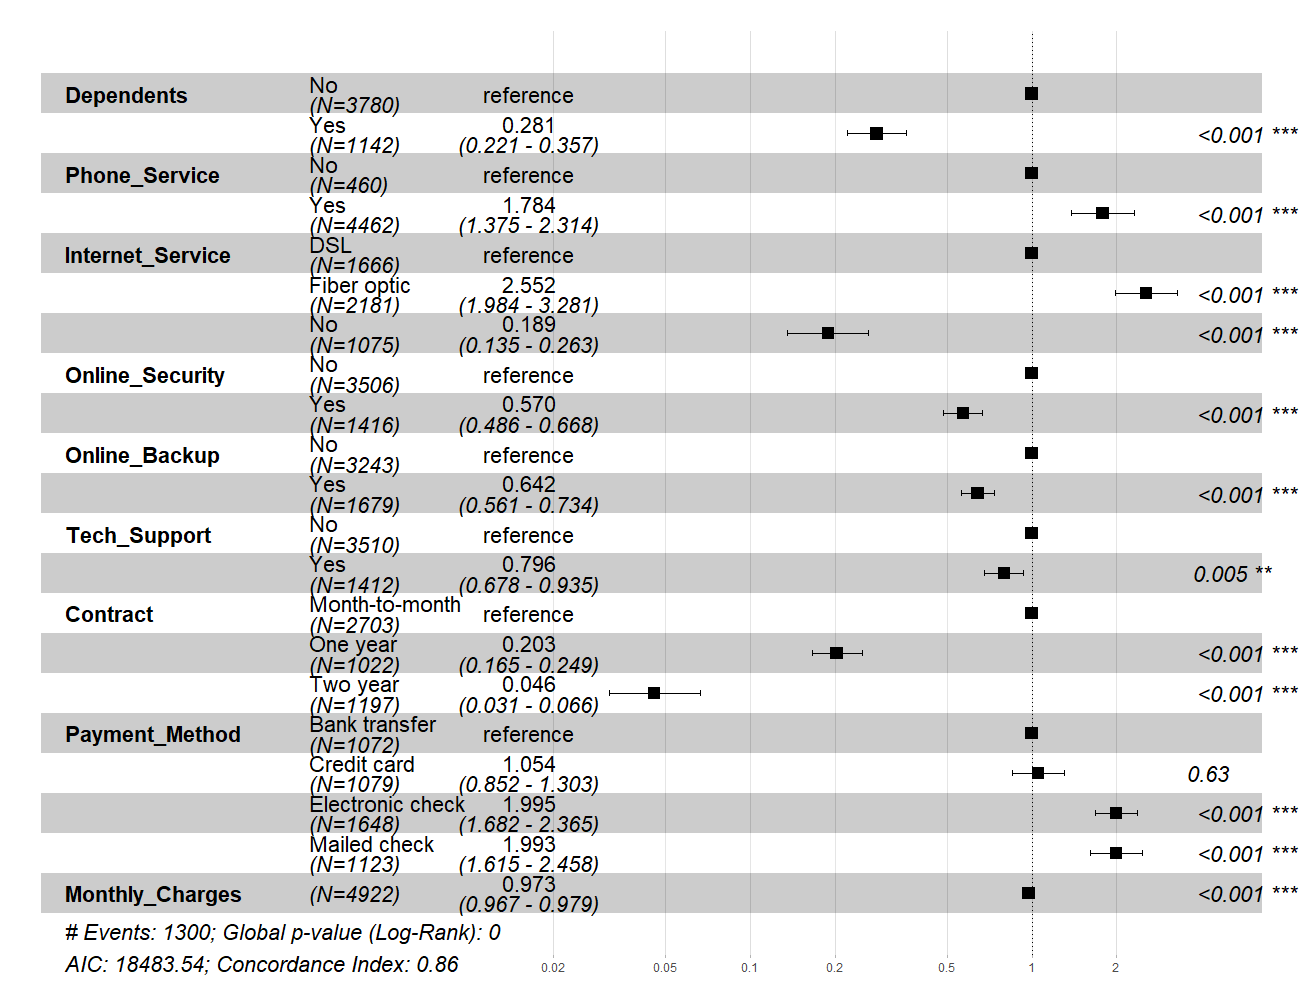
\includegraphics[width=18.06in]{./imgs/cox_ggforest} 

}

\caption{Marginal effects obtained with the Cox PH model}\label{fig:coxmarginaleffects}
\end{figure}

\hypertarget{estimation-results}{%
\subsubsection*{Estimation results}\label{estimation-results}}
\addcontentsline{toc}{subsubsection}{Estimation results}

Semi-parametric models aims at estimating the instantaneous hazard function given a baseline hazard and a set of covariates. The model outputs a risk prediction for each individual with a confidence interval. Then, the survival and cumulative hazard functions can be retrieved as explained in section \ref{probabilities}. When going deeper into the functions depicted in figure \ref{fig:coxdataviz}, it can be noticed some inconsistencies between the estimated churn hazard cumulative hazard functions. Given the cumulative churn hazard increases faster when the number of months is high and given the instantaneous hazard is supposed to be the cumulative hazard function's slope, the estimated churn hazard's shape should be convex. Thus, the Cox model does not manage to properly estimate the risk of churn.

\begin{figure}

{\centering 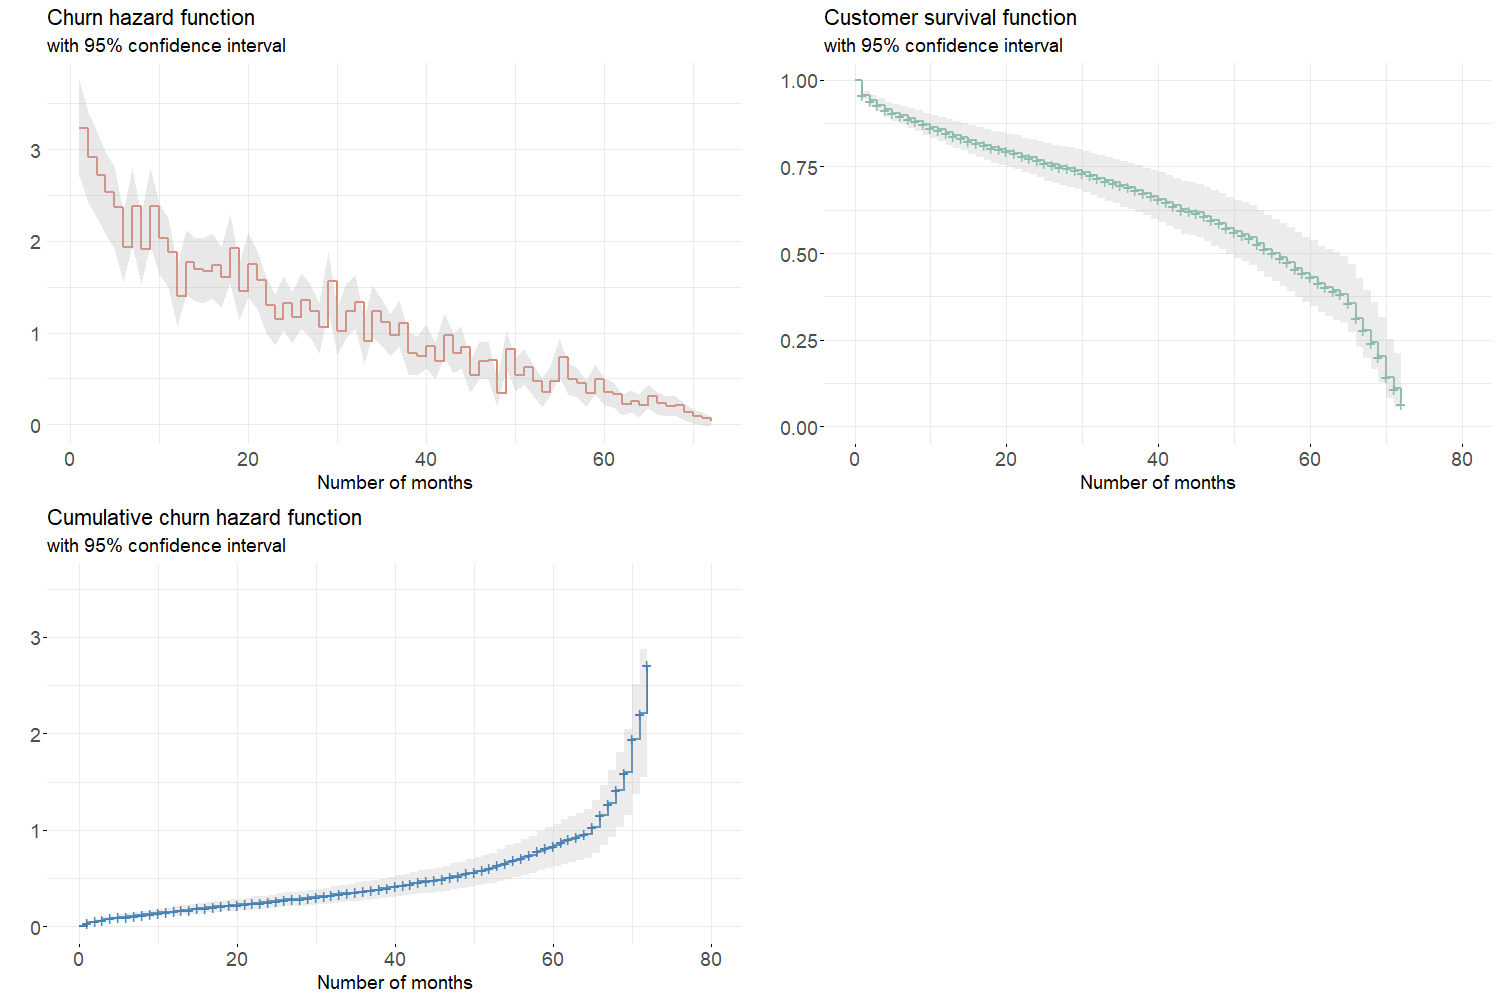
\includegraphics[width=20.83in]{./imgs/cox_data_viz} 

}

\caption{Aggregated churn hazard, survival and cumulative hazard functions estimated by Cox model}\label{fig:coxdataviz}
\end{figure}

Although the fitted model is not flawless, it can be interested to study the estimation differences between the 3 customer segments identified in the previous section. Looking at figure \ref{fig:coxclust}, one can conclude that \emph{Gold} (cluster 2) clients are more prone to churn than others. The aggregated risk of attrition is indeed higher to such an extent that the cumulative churn hazard is exploding when the number of months is greater than 60. This being said, an efficient portfolio management would be to find strategies to reduce \emph{Gold} customers' churn and increase their duration in the portfolio.

\begin{figure}

{\centering 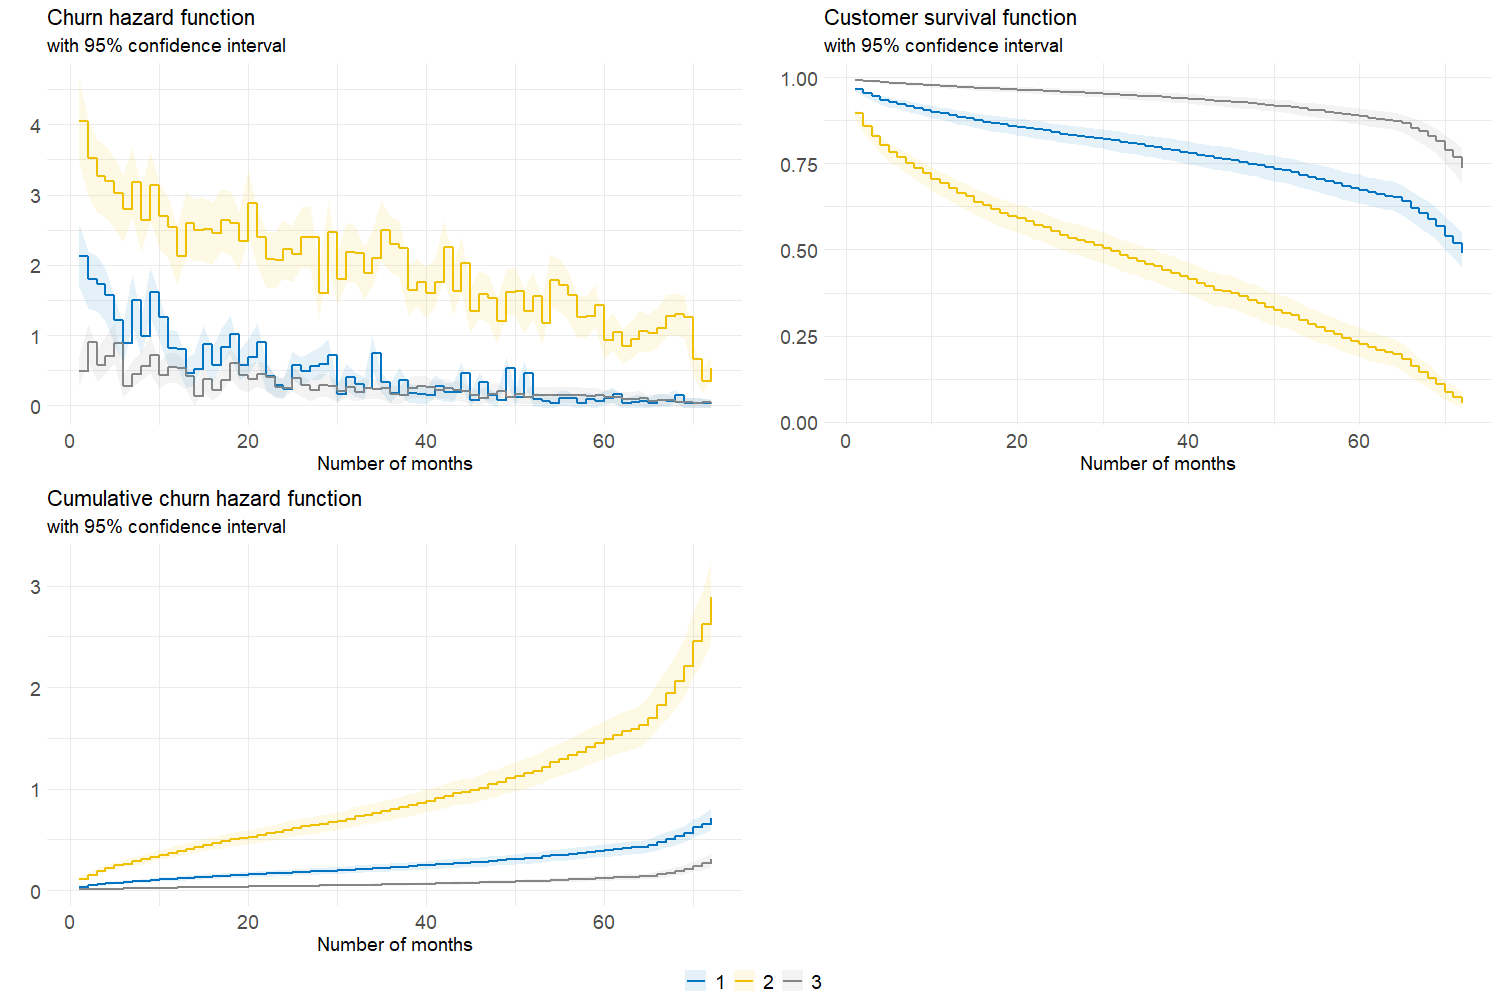
\includegraphics[width=20.83in]{./imgs/churn_surv_clust} 

}

\caption{Aggregated churn hazard, survival and cumulative hazard functions for each cluster}\label{fig:coxclust}
\end{figure}

\hypertarget{other-survival-models}{%
\subsection{Other survival models}\label{other-survival-models}}

As said in the previous part, the Cox model does not fit the data perfectly as it does not capture the churn hazard's actual shape. In this context, it seems relevant to fit other survival models and test how they perform in predicting the risk of attrition. It is firstly decided to train parametric survival models which consist in assigning a probability distribution to the hazard function (see section \ref{parametric} for more details). To that end, one can use \texttt{flexsurv} \citep{flexsurv2016} which is and R package for parametric survival modelling. After having fitted the exponential, Weibull, gamma, log-logistic and log-normal models, no improvement can be observed with respect to the Cox model. Then, a machine learning approach can be adopted to model duration data using the random survival forest algorithm as explained in section \ref{mlsurv}. The \texttt{rfsrc} function from \texttt{randomForestSRC} \citep{randomForestSRC2008} is used to train the model after having determined the optimal node size and number of variables to try at each split with the \texttt{tune} function. Once the model trained, its performance is compared to the Cox model's as shown by table \ref{tab:performances}. One cannot but admit that the random survival forest perform poorly in terms of concordance index with respect to the Cox model. The latter manages to output a better risk scoring than the ML algorithm. It is thus decided to select the Cox PH model for the rest of the study.

\textbackslash begin\{table\}{[}H{]}

\textbackslash caption\{\label{tab:performances}Concordance index (\%) obtained with Cox model and Random Survival Forest (RSF)\}
\centering

\begin{tabular}[t]{lrr}
\toprule
  & Train & Test\\
\midrule
\cellcolor{gray!6}{Cox} & \cellcolor{gray!6}{86.769} & \cellcolor{gray!6}{86.253}\\
RSF & 49.273 & 49.229\\
\bottomrule
\end{tabular}

\textbackslash end\{table\}

\hypertarget{portfolio-value-estimation}{%
\section{Portfolio value estimation}\label{portfolio-value-estimation}}

In the two previous sections, the portfolio has been partitioned into 3 customer segments and customer lifetime has been estimated by the means of the Cox model. This section's purpose consists in deriving a method to calculate the overall value of the portfolio through the computation of customer lifetime raw value.

\hypertarget{the-model}{%
\subsection{The model}\label{the-model}}

As said in chapter \ref{data}, it is decided not to use the \texttt{CLTV} variable to estimate customer lifetime value since no information has been provided on the computation method. Instead, another method is adopted to predict each client's lifetime value. For this purpose, two inputs are needed namely each customer's survival function as well as the monthly fees represented by the \texttt{Monthly\_Charges} feature. Based on the CLV formulation proposed by Gupta and Lehmann \citep{CUSTOMERS_ASSETS}, we derive a model aiming at calculating customer lifetime raw value (CLRV) as depicted in equation \eqref{eq:clrv}.

\begin{equation}
    \text{CLRV}_i = \sum_{t=0}^{T} \frac{p_i \ r_{i,t}}{(1+a)^t} 
    \label{eq:clrv}
\end{equation}

with,

\begin{itemize}
\tightlist
\item
  \(p_i\) the monthly fee paid by customer \(i\),
\item
  \(r_{i,t}\) the probability that customer \(i\) be in the portfolio at time \(t\),
\item
  \(a\) the discount factor,
\item
  \(T\) the time horizon.
\end{itemize}

It may be interesting to note that \(p_i\) is time-invariant and corresponds to \texttt{Monthly\_Charges}. \(r_{i,t}\) is computed using the survival function estimated with the Cox model. \(a\) is fixed at 8\% and \(T\) equals 72 months which is the longest lifetime in the data.

Summing over the \(N\) CLRVs, one can derive customer raw equity which is the portfolio raw value (V) and may be a good proxy for the firm's overall revenues.

\begin{equation}
    \text{V} = \sum_{i=1}^{N} \text{CLRV}_i = \sum_{i=1}^{N} \sum_{t=0}^{T} \frac{p_i \ r_{i,t}}{(1+a)^t} 
    \label{eq:cre}
\end{equation}

\hypertarget{customer-lifetime-raw-value}{%
\subsection{Customer Lifetime Raw Value}\label{customer-lifetime-raw-value}}

In the literature, it is common place to measure customer lifetime value that is the overall profit brought by a client over her entire lifetime in the portfolio. In our study, the data set used does not provide any information on the costs related to each customer. Consequently, it is decided to evaluate customer value by computing the overall revenues the firm might earn during the relationship with their clients. We name this metric customer lifetime raw value (CLRV) and it is defined in equation \eqref{eq:clrv}.

The process implemented to compute client \(i\)'s CLRV works as follows:

\begin{enumerate}
\def\labelenumi{\arabic{enumi}.}
\tightlist
\item
  Estimate client \(i\)'s survival function over 72 months using the Cox model fitted in section \ref{coxmodel}.
\item
  For each month, multiply the value of the survival function by the monthly fee \(p_i\) paid by client \(i\). Then, divide the product by \((1 + a)^t\) where \(t\) is the month's index and \(a\) the discount factor.
\item
  Take the sum of the \(T\) ratios.
\end{enumerate}

Since the data is made up of more than 7,000 customers and given the CLRV calculation is time consuming, parallelization has been used to calculate every CLRV. Once all the CLRVs are computed, one may take the sum in order to retrieve the portfolio's global value as well as a 95\% confidence interval as shown by table \ref{tab:custValuesSum}.

\begin{table}[H]

\caption{\label{tab:custValuesSum}Portfolio estimated value with 95$\%$ confidence interval}
\centering
\begin{tabular}[t]{llll}
\toprule
  & V lower & V & V upper\\
\midrule
\cellcolor{gray!6}{} & \cellcolor{gray!6}{17,604,144} & \cellcolor{gray!6}{18,270,000} & \cellcolor{gray!6}{19,031,648}\\
\bottomrule
\end{tabular}
\end{table}

Going deeper into the statistical analysis of customer lifetime raw value, it can be noticed from table \ref{tab:custValuesStats} and figure \ref{fig:clrvDens} that the clients are quite heterogeneous. The distribution of CLRV is left-skewed with a median lower than the mean. In addition, the CLRV ranges from 324 to 6815 indicating that each client does not have the same value to the firm.

\begin{figure}

{\centering 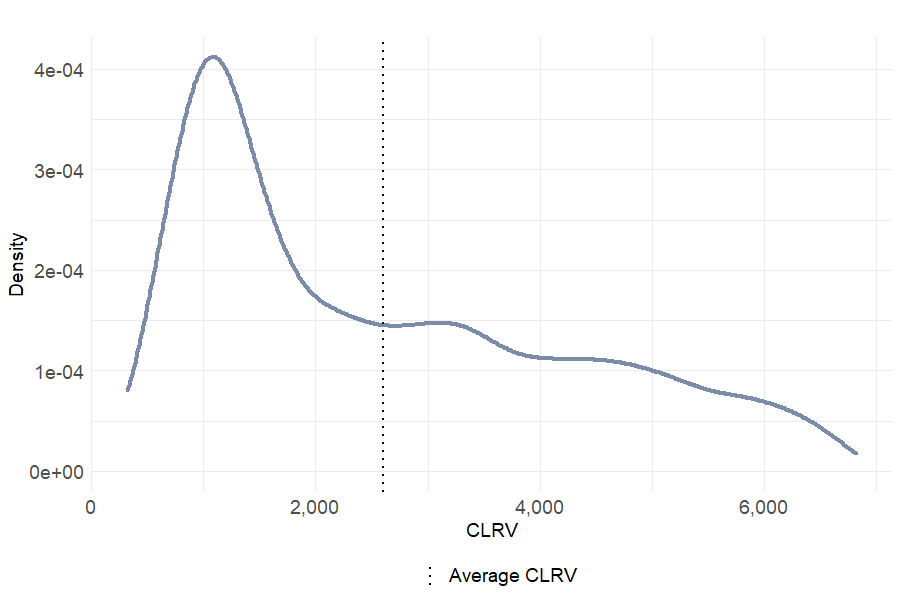
\includegraphics[width=12.5in]{./imgs/clrv_density} 

}

\caption{Distribution of Customer Lifetime Raw Value}\label{fig:clrvDens}
\end{figure}

\begin{table}[H]

\caption{\label{tab:custValuesStats}CLRV Statistical summary}
\centering
\begin{tabular}[t]{lrrrrrr}
\toprule
  & Min. & 1st Qu. & Median & Mean & 3rd Qu. & Max.\\
\midrule
\cellcolor{gray!6}{} & \cellcolor{gray!6}{323.99} & \cellcolor{gray!6}{1125.9} & \cellcolor{gray!6}{2104.66} & \cellcolor{gray!6}{2598.12} & \cellcolor{gray!6}{3850.41} & \cellcolor{gray!6}{6815.42}\\
\bottomrule
\end{tabular}
\end{table}

Eventually, it seems interesting to visualize the contribution of each month to customer lifetime raw value. Based on figure \ref{fig:clrvEvolution}, the montlhy contribution decreases as the number of months increases which leads to a concave cumulative value. This result may be explained by the increase in \((1+a)^t\) and the decrease in the survival probability \(r_{i,t}\) as \(t\) increases (see equation \eqref{eq:clrv}). In other words, customers bring in more value to the firm at the beginning of the relationship.

\begin{figure}

{\centering 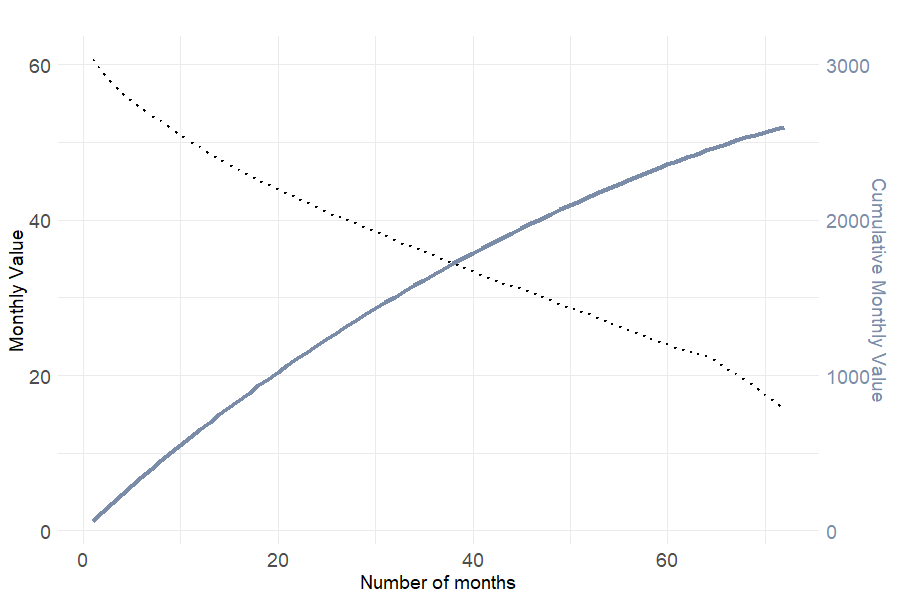
\includegraphics[width=12.5in]{./imgs/clrv_evolution} 

}

\caption{Monthly contribution and cumulative value depending on the number of months in the portfolio}\label{fig:clrvEvolution}
\end{figure}

\hypertarget{cluster-contribution-to-the-portfolio-value}{%
\subsection{Cluster contribution to the portfolio value}\label{cluster-contribution-to-the-portfolio-value}}

In section \ref{segmentation}, 3 clusters of customers have been identified using hierarchical clustering. This being said, it is undoubtedly necessary to calculate the value of each group using the method presented above. The following table depicts each cluster's CLRV with 95\% confidence interval as well as the \% proportion in terms of number of clients and \% contribution in terms of value. One can notice that the \emph{Platinum} cluster accounts for more than half the portfolio total value even if it represents barely a third of the number of clients. Besides, \emph{Silver} customers are the less valuable to the firm as their contribution barely amounts to a 12\%. Recall that this group is characterized by a minimum subscription with no internet connection or additional services. Finally, the \emph{Gold} segment's contribution is \(\approx\) 40\% lower than cluster 3's. It may be explained by cluster 2 client's higher propensity to churn.

\begin{table}[H]

\caption{\label{tab:totValclust}Total CLRV per cluster}
\centering
\begin{tabular}[t]{>{}cccccc}
\toprule
Cluster & Proportion (\%) & V lower & V & V upper & Contribution (\%)\\
\midrule
\em{\cellcolor{gray!6}{Silver (1)}} & \cellcolor{gray!6}{26.6} & \cellcolor{gray!6}{2,035,928} & \cellcolor{gray!6}{2,117,932} & \cellcolor{gray!6}{2,213,746} & \cellcolor{gray!6}{11.59}\\
\em{Gold (2)} & 41.4 & 5,760,579 & 6,211,027 & 6,734,243 & 34.00\\
\em{\cellcolor{gray!6}{Platinum (3)}} & \cellcolor{gray!6}{32.1} & \cellcolor{gray!6}{9,807,637} & \cellcolor{gray!6}{9,941,041} & \cellcolor{gray!6}{10,083,660} & \cellcolor{gray!6}{54.41}\\
\bottomrule
\end{tabular}
\end{table}

Once the value differences across clusters identified, let us dig into a more detailed analysis of customer value based on the group they belong to. On figure \ref{fig:clrvDensClust}, the 3 CLRV distributions indicate large disparities between each client segment. While cluster 1 customers are defined an inflation of values located before 2,000, the two other groups are more homogeneous. The CLRV of cluster 2 (respectively 3) clients seems evenly distributed between 0 (respectively 1,500) and 6,000 (respectively 7,000).

\begin{figure}

{\centering 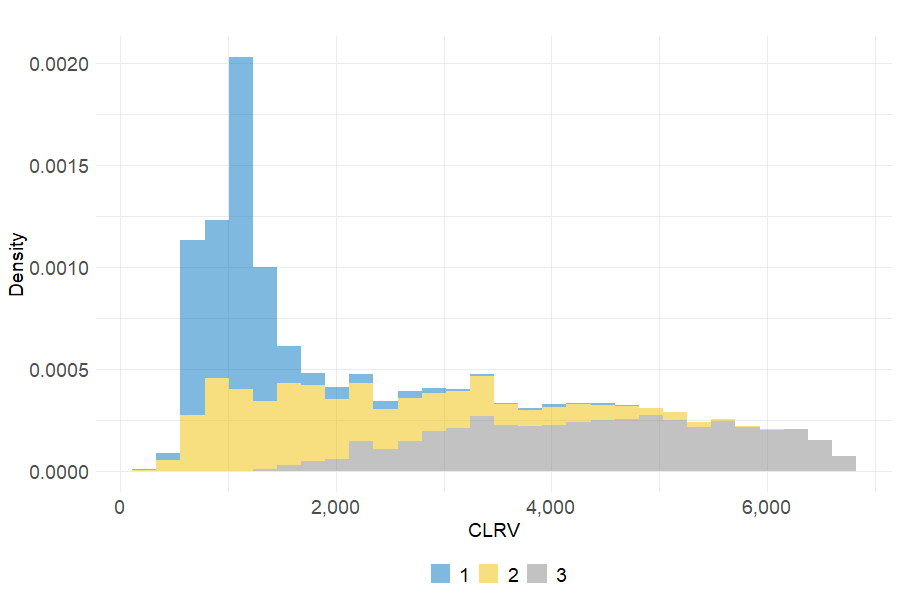
\includegraphics[width=12.5in]{./imgs/clrv_density_per_cluster} 

}

\caption{Distribution of Customer Lifetime Raw Value per cluster}\label{fig:clrvDensClust}
\end{figure}

\begin{table}[H]

\caption{\label{tab:custValuesclust}CLRV statistical summary for each customer segment}
\centering
\begin{tabular}[t]{>{}lcccccc}
\toprule
  & Min. & 1st Qu. & Median & Mean & 3rd Qu. & Max.\\
\midrule
\em{\cellcolor{gray!6}{Silver (1)}} & \cellcolor{gray!6}{333.82} & \cellcolor{gray!6}{837.50} & \cellcolor{gray!6}{1094.51} & \cellcolor{gray!6}{1134.40} & \cellcolor{gray!6}{1264.28} & \cellcolor{gray!6}{4679.80}\\
\em{Gold (2)} & 323.99 & 1194.59 & 1862.16 & 2134.37 & 2886.02 & 6009.78\\
\em{\cellcolor{gray!6}{Platinum (3)}} & \cellcolor{gray!6}{1268.74} & \cellcolor{gray!6}{3393.93} & \cellcolor{gray!6}{4489.62} & \cellcolor{gray!6}{4408.44} & \cellcolor{gray!6}{5454.71} & \cellcolor{gray!6}{6815.42}\\
\bottomrule
\end{tabular}
\end{table}

When looking at table \ref{tab:custValuesclust}, large variations appear between each cluster's average CLRV. With a view of testing whether these differences are significant, the ANOVA test is performed between the \texttt{CLRV} and \texttt{cluster} variables. The very low p-value depicted in the table below indicates significant different means across the 3 groups. Hence, it can be affirmed that the contribution of each client segment to the portfolio value is statistically different.

\begin{table}[H]

\caption{\label{tab:aov}Results of the ANOVA test between CLRV and cluster}
\centering
\begin{tabular}[t]{lccccc}
\toprule
  & Df & Sum of squares & MSE & F value & P value\\
\midrule
\cellcolor{gray!6}{Cluster} & \cellcolor{gray!6}{2} & \cellcolor{gray!6}{12,016,055,579} & \cellcolor{gray!6}{6,008,027,789} & \cellcolor{gray!6}{5,205.39} & \cellcolor{gray!6}{0}\\
Residuals & 7029 & 8,112,831,034 & 1,154,194 &  & \\
\bottomrule
\end{tabular}
\end{table}

With the objective of determining how each group's representative customer differ one from another in terms of CLRV, it seems a good idea to visualize the evolution of their respective cumulative value as the number of months in the portfolio increases. Figure \ref{fig:clrvEvolutionClust} shows that the lower value to the firm, the flatter curve. To put it another way, \emph{Silver} clients' monthly contribution to CLRV decreases rapidly and becomes constantly low after 30 months. On the contrary, \emph{Platinum} customers bring in a larger monthly value and the latter decreases to a lesser extent. As for \emph{Gold} customers, their cumulative value becomes nearly constant from month 40 which may be due to their lower loyalty to the firm.

\begin{figure}

{\centering 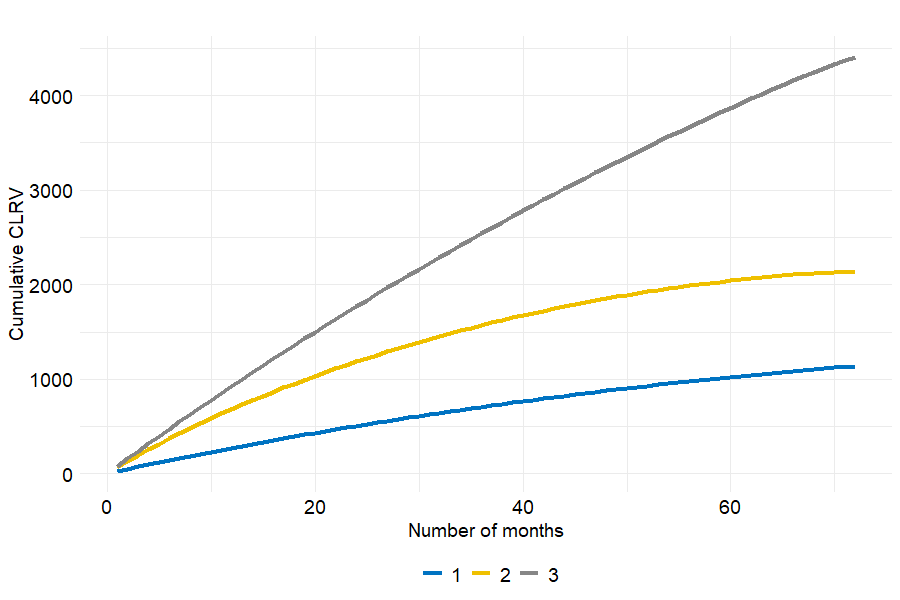
\includegraphics[width=12.5in]{./imgs/clrv_evolution_per_cluster} 

}

\caption{Customer cumulative value through time per cluster}\label{fig:clrvEvolutionClust}
\end{figure}

\hypertarget{simulations}{%
\subsection{Simulations}\label{simulations}}

The final step in our study aims at simulating different multiple scenarios to determine how customer lifetime raw value and the portfolio value might evolve \emph{ceteris paribus}. This section is not exhaustive in inasmuch as only a few parameters have been selected to perform the simulations.

\hypertarget{influence-of-the-discount-factor-on-clrv}{%
\subsubsection*{Influence of the discount factor on CLRV}\label{influence-of-the-discount-factor-on-clrv}}
\addcontentsline{toc}{subsubsection}{Influence of the discount factor on CLRV}

In the CLRV formula (equation \eqref{eq:clrv}), the discount factor \(a\) plays a central role since it monitors the importance of future values in the customer value. In this context, it is decided to analyse the evolution of both CLRV and portfolio value after a change in \(a\). The simulation results reproduced in table \ref{tab:portValDiscountTab} lead us to suppose that the portfolio overall value decreases as the discount factor increases. V is indeed reduced by almost 16\% when \(a\) goes from 1\% to 8\%.

\begin{table}[H]

\caption{\label{tab:portValDiscountTab}Portfolio value depending on discount rate}
\centering
\begin{tabular}[t]{llll}
\toprule
  & V Lower & V & V upper\\
\midrule
\cellcolor{gray!6}{1\%} & \cellcolor{gray!6}{20,894,006} & \cellcolor{gray!6}{21,721,297} & \cellcolor{gray!6}{22,674,662}\\
2\% & 20,358,160 & 21,158,861 & 22,080,569\\
\cellcolor{gray!6}{4\%} & \cellcolor{gray!6}{19,357,495} & \cellcolor{gray!6}{20,108,832} & \cellcolor{gray!6}{20,971,852}\\
8\% & 17,604,144 & 18,270,000 & 19,031,648\\
\bottomrule
\end{tabular}
\end{table}

The reduction in V after an increase in the discount rate is actually the direct consequence of a decrease in every customer lifetime raw value. The monthly contribution to CLRV being negatively influenced by \(a\) as the number of months \(t\) increases, this phenomenon is all the more pronounced when \(a\) is large. On figure \ref{fig:clrvEvolDiscount}, one can observe that the higherthe discount factor, the more concave the shape of the cumulative value. In other words the higher the discount factor, the lower gain in CLRV when the number of months is high.

\begin{figure}

{\centering 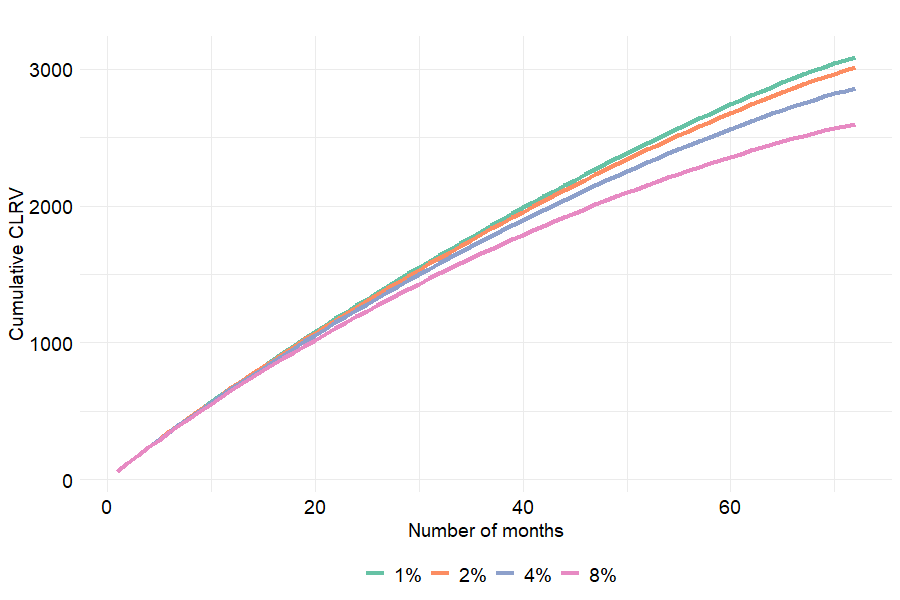
\includegraphics[width=12.5in]{./imgs/clrv_evolution_discount} 

}

\caption{Customer Lifetime Raw Value evolution depending on discount rate}\label{fig:clrvEvolDiscount}
\end{figure}

\hypertarget{influence-of-month-to-month-contracts-on-clrv}{%
\subsubsection*{Influence of month-to-month contracts on CLRV}\label{influence-of-month-to-month-contracts-on-clrv}}
\addcontentsline{toc}{subsubsection}{Influence of month-to-month contracts on CLRV}

While it is obviously doable to simulate new customer lifetime raw values by playing with the model's parameters, one can also change the values of covariates used to estimate the survival probabilities \(r_{i,t}\). In this part, the analysis is centred on the proportion of month-to-month contracts in the portfolio. The method consists in computing each client's CLRV and the portfolio value V for proportions of monthly contracts ranging from 10 to 90\%. Table \ref{tab:portValmonthToMonth} examines the portfolio value for 4 interesting scenarios and compare them with the actual share of month-to-month contracts in the data. The results are quite counter-intuitive as V is not maximum for a 10\% proportion whereas it has been demonstrated in figure \ref{fig:coxmarginaleffects} that clients enrolled in month-to-month contracts are 22 times more prone to churn than those with two-year contracts. Hence one might think that the lower share of those customers, the higher value of the portfolio.

\textbackslash begin\{table\}{[}H{]}

\textbackslash caption\{\label{tab:portValmonthToMonth}Portfolio estimated value and 95\% confidence interval depending on proportion of month-to-month contracts\}
\centering

\begin{tabular}[t]{llll}
\toprule
\% month-to-month contracts & V lower & V & V upper\\
\midrule
\cellcolor{gray!6}{10\%} & \cellcolor{gray!6}{22,526,500} & \cellcolor{gray!6}{23,009,290} & \cellcolor{gray!6}{23,535,331}\\
30\% & 24,289,738 & 25,001,468 & 25,801,858\\
\cellcolor{gray!6}{70\%} & \cellcolor{gray!6}{19,763,605} & \cellcolor{gray!6}{20,706,782} & \cellcolor{gray!6}{21,796,005}\\
90\% & 18,266,063 & 19,369,938 & 20,646,166\\
\cellcolor{gray!6}{55.1\% (reference)} & \cellcolor{gray!6}{17,604,144} & \cellcolor{gray!6}{18,270,000} & \cellcolor{gray!6}{19,031,648}\\
\bottomrule
\end{tabular}

\textbackslash end\{table\}

The following figure illustrates the CLRV distribution for 4 scenarios depending on the proportion of month-to-month contracts. The results are closer to our expectations than those presented in the previous table since CLRV tends to be higher when there are 10\% month-to-month contracts in the portfolio.

\begin{figure}

{\centering 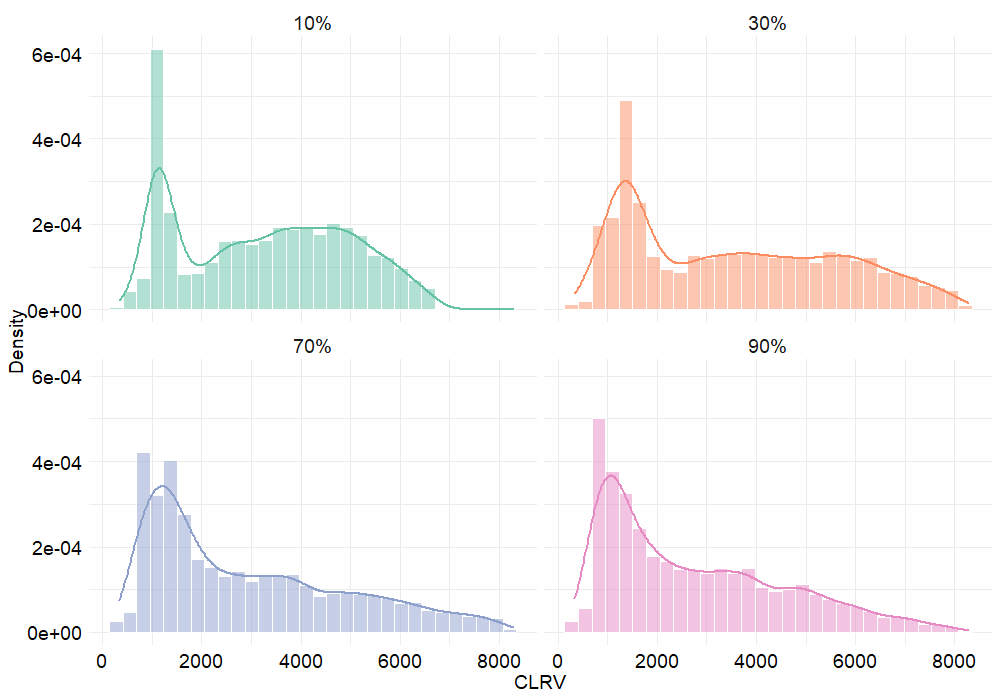
\includegraphics[width=13.89in]{./imgs/clrv_month_to_month} 

}

\caption{CLRV distribution depending on the proportion of month-to-month contracts}\label{fig:clrvmonthtomonth}
\end{figure}

Ultimately when representing the evolution of customer raw equity, i.e.~the portfolio value, according to the share of month-to-month contracts, a decreasing trend is identified which appears to be a rational result.

\begin{figure}

{\centering 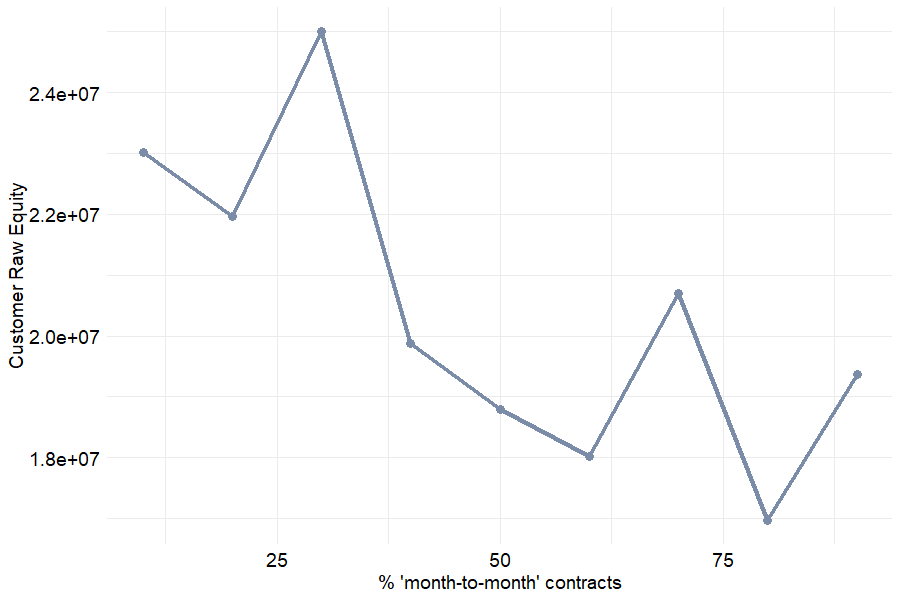
\includegraphics[width=12.5in]{./imgs/portVal_month_to_month} 

}

\caption{Portfolio estimated value (Customer Raw Equity) depending on the proportion of month-to-month contracts}\label{fig:clrvmonthtomonthEvol}
\end{figure}

\hypertarget{how-to-increase-customer-lifetime-raw-value}{%
\subsubsection*{How to increase Customer Lifetime Raw Value?}\label{how-to-increase-customer-lifetime-raw-value}}
\addcontentsline{toc}{subsubsection}{How to increase Customer Lifetime Raw Value?}

At this point of the study, a consistent method to evaluate the firm's portfolio value through the computation of customer lifetime raw value has been implemented. In section \ref{churnAnalysis} it has been shown that customers from the \emph{Gold} cluster are characterized by a higher churn rate and lower survival probabilities. This lesser loyalty to the firm has a negative impact on the portfolio value. Furthermore, cluster 2 clients amount to 34\% in the customer raw equity which proves their strong potential in terms of CLRV. Therefore, a method to increase \emph{Gold} customers' lifetime is proposed in this last section. To that end, it is decided to offer additional services for free to every cluster 2 client. These services are represented by the following variables: \texttt{Online\_Security}, \texttt{Online\_Backup} and \texttt{Tech\_Support}. The underlying purpose is to increase the survival probabilities estimated by the Cox model as it has been proved that they have a negative impact on the churn hazard (see figure \ref{fig:coxmarginaleffects}).

The results presented in the table below support our hypothesis since the \emph{Gold} cluster total value increases by almost 50\% after having provided the clients with free additional options.

\begin{table}[H]

\caption{\label{tab:unnamed-chunk-32}Increase in portfolio value after having provided cluster 2 clients with additional services}
\centering
\begin{tabular}[t]{llr}
\toprule
  & Cluster 2 Value & \% Variation\\
\midrule
\cellcolor{gray!6}{Reference} & \cellcolor{gray!6}{6,211,027} & \cellcolor{gray!6}{0.00}\\
With additional options & 9,218,937 & 48.43\\
\bottomrule
\end{tabular}
\end{table}

Figure \ref{fig:clust2CLRV} illustrates the mechanism that leads to an increase in the portfolio value after the ``gift'' to cluster 2 clients. One can notice a significant shift to the right of the CLRV distribution. This shift is the consequence of an increase in \(r_{i,t}\) - client \(i\)'s survival probability at time \(t\) - which is a positive driver of customer value. We are thus able to propose a marketing strategy which aims at boosting the firm's lifetime revenues. Note, however, that our methodology does not take costs into account which implies that the highlighted points should be mitigated.

\begin{figure}

{\centering 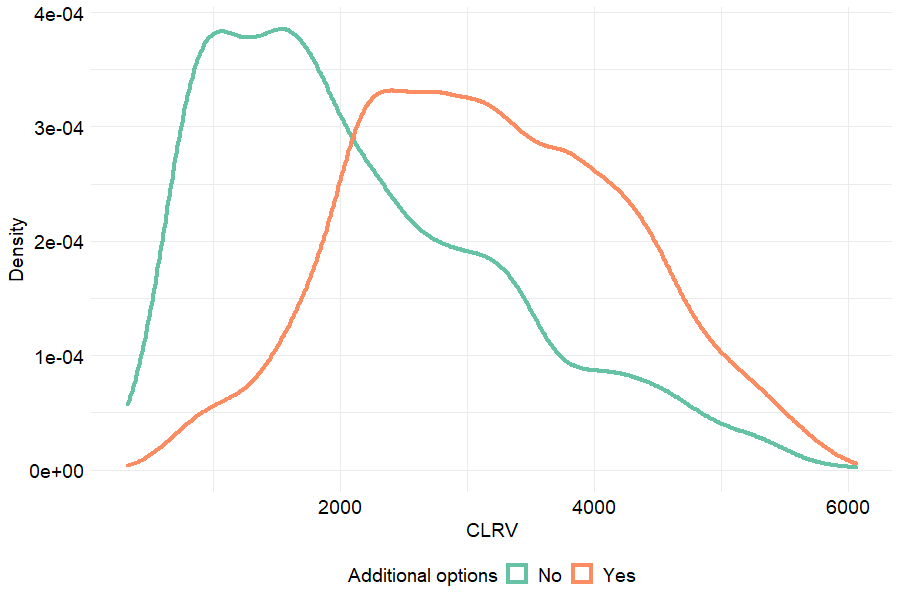
\includegraphics[width=12.5in]{./imgs/clust2_clrv} 

}

\caption{Increase in cluster 2 clients' CLRV after after having provided them with additional services}\label{fig:clust2CLRV}
\end{figure}

\hypertarget{conclusion}{%
\chapter*{Conclusion}\label{conclusion}}
\addcontentsline{toc}{chapter}{Conclusion}

Our study on customer \emph{portfolio}, \emph{attrition} and customer \emph{value} has a threefold purpose. To begin with, the literature review helps the readers to understand the important notions behind the topic's key points. Although it is far from being exhaustive, it summarizes the important Econometrics and Data Science improvements that have been made in terms of portfolio management, churn analysis and customer value estimation. Secondly, a large part of the study centers on the theoretical foundations of duration models which are essential to predict the risk of churn. Finally, chapter \ref{estimation} explains the ins and outs of a decision support tool whose goal is to manage a portfolio of customers. The method consists in identifying groups of customers who have similar consumption habits, then estimating customer lifetime by the means of duration models to eventually calculate the overall lifetime value of the portfolio based on the computation of customer lifetime raw value.

Nevertheless, some improvements need to be made in order to make our project more consistent to be applied in a business context. The Cox model introduced in section \ref{churnAnalysis} presents some limitations since it does not manage to properly estimate the risk of churn. A more reliable estimation method might be adopted such as more complex parametric models or machine learning algorithms for survival data. In addition, it could be relevant to determine the churn reason using competing risk models. As for the data, we think our study would be more impactful with time-varying covariates and more observations. Eventually, as said at the end of the previous chapter, costs are not taken into account in the estimation method. An area for improvement might be to add simulated costs to the data set or retrieving online data on the costs of telecommunication service providers.

\hypertarget{appendix}{%
\chapter*{Appendix}\label{appendix}}
\addcontentsline{toc}{chapter}{Appendix}

In this section some proofs of the mathematical concepts used in the study are derived, specifically related to duration analysis. It also consists of additional data visualisation related to the chapter \ref{estimation}.

\hypertarget{hazard-function}{%
\section*{Hazard function}\label{hazard-function}}
\addcontentsline{toc}{section}{Hazard function}

\begin{equation}    
  \begin{aligned}
  \lambda(t) & = \lim_{\Delta t \to 0} \frac{P\big[t \leq T < t + \Delta t | T \geq t \big]}{\Delta t} \\\\
  & = \lim_{\Delta t \to 0} \frac{P\big[t \leq T < t + \Delta t \big] / P\big[T \geq t  \big]}{\Delta t} \\\\
  & = \lim_{\Delta t \to 0} \frac{\big(F(t+\Delta t)-F(t)\big) / \Delta t}{S(t)} \\\\
  & = \frac{\text{d} F(t) / \text{d} t}{S(t)} \\\\
  & = \frac{f(t)}{S(t)} \\\\
  & = - \frac{\text{d}S(t) / \text{d} t}{S(t)} \\\\
  \lambda(t) & = \frac{-\text{d} \ln \big(S(t)\big)}{\text{d} t}
  \end{aligned}
  \label{eq:hazfunproof}
\end{equation}

\hypertarget{link-between-cumulative-hazard-and-survivor-functions}{%
\section*{Link between cumulative hazard and survivor functions}\label{link-between-cumulative-hazard-and-survivor-functions}}
\addcontentsline{toc}{section}{Link between cumulative hazard and survivor functions}

\begin{equation}
  \begin{aligned}
       & \Lambda(t) = \int_{0}^{t} \lambda(s)ds \\\\
  \iff & \Lambda(t) = \int_{0}^{t} \frac{f(s)}{S(s)}ds \\\\
  \iff & \Lambda(t) = -\ln \big(S(t)\big) \\\\
  \iff & S(t) = \exp \big(-\Lambda(t)\big)
  \end{aligned}
  \label{eq:linksurvcumhaz}
\end{equation}

\hypertarget{contribution-to-the-partial-likelihood-function-in-ph-models}{%
\section*{Contribution to the partial likelihood function in PH models}\label{contribution-to-the-partial-likelihood-function-in-ph-models}}
\addcontentsline{toc}{section}{Contribution to the partial likelihood function in PH models}

\begin{equation}
\begin{aligned}
  \mathbb{P}\big[T_j = t_j | R(t_j) \big] & = \frac{\mathbb{P}\big[T_j = t_j | T_j \geq t_j \big]}{\sum_{l \in R(t_j)} \ \mathbb{P}\big[T_l = t_l | T_l \geq t_j \big]} \\\\
  & = \frac{\lambda_j(t_j|\mathrm{x_j}, \beta)}{\sum_{l \in R(t_j)} \ \lambda_l(t_l|\mathrm{x_l}, \beta)} \\\\
  & = \frac{\lambda_0 (t_j, \alpha)\phi(\mathrm{x_j}, \beta)}{\sum_{l \in R(t_j)} \ \lambda_0 (t_j, \alpha)\phi(\mathrm{x_l}, \beta)} \\\\
  \mathbb{P}\big[T_j = t_j | R(t_j) \big] & = \frac{\phi(\mathrm{x_j}, \beta)}{\sum_{l \in R(t_j)} \phi(\mathrm{x_l}, \beta)}
\end{aligned}
\label{eq:contribpartiallikproof}
\end{equation}

\hypertarget{partial-likelihood-function-in-ph-models}{%
\section*{Partial likelihood function in PH models}\label{partial-likelihood-function-in-ph-models}}
\addcontentsline{toc}{section}{Partial likelihood function in PH models}

Based on equation \eqref{eq:contribpartiallik}, one can derive the probability that all spells completed at \(t_j\) ends in the \(j^{\text{th}}\) failure time, such that:

\begin{equation}
\begin{aligned}
  \mathcal{L}_{p,\ t_j} & = \mathbb{P}\big[T_1 = t_j, \dots, T_{d_j} = t_j \ | \ R(t_j)\big] \\\\
  & = \Pi_{m \in D(t_j)} \ \mathbb{P}\big[T_m = t_j | R(t_j) \big] \\\\
  & = \Pi_{m \in D(t_j)} \ \frac{\phi(\mathrm{x_m}, \beta)}{\sum_{l \in R(t_j)} \phi(\mathrm{x_l}, \beta)} \\\\
  & = \Pi_{m \in D(t_j)} \ \phi(\mathrm{x_m}, \beta) \times \Pi_{m \in D(t_j)} \ \frac{1}{\sum_{l \in R(t_j)} \phi(\mathrm{x_l}, \beta)} \\\\
  \mathcal{L}_{p,\ t_j} & = \frac{\Pi_{m \in D(t_j)} \ \phi(\mathrm{x_m}, \beta)}{\Big[\sum_{l \in R(t_j)} \phi(\mathrm{x_l}, \beta)\Big]^{d_j}}
\end{aligned}
\label{eq:partlikproof}
\end{equation}

The joint probability over the \(k\) ordered discrete failure times then becomes:

\begin{equation}
\begin{aligned}
  \mathcal{L}_p & = \Pi_{j=1}^{k} \ \mathcal{L}_{p,\ t_j} \\\\
  \mathcal{L}_p & = \Pi_{j=1}^{k} \ \frac{\Pi_{m \in D(t_j)} \ \phi(\mathrm{x_m}, \beta)}{\Big[\sum_{l \in R(t_j)} \phi(\mathrm{x_l}, \beta)\Big]^{d_j}}
\end{aligned}
\label{eq:partlikproofbis}
\end{equation}

\hypertarget{mcaappendix}{%
\section*{Multiple correspondence analysis}\label{mcaappendix}}
\addcontentsline{toc}{section}{Multiple correspondence analysis}

\begin{figure}

{\centering 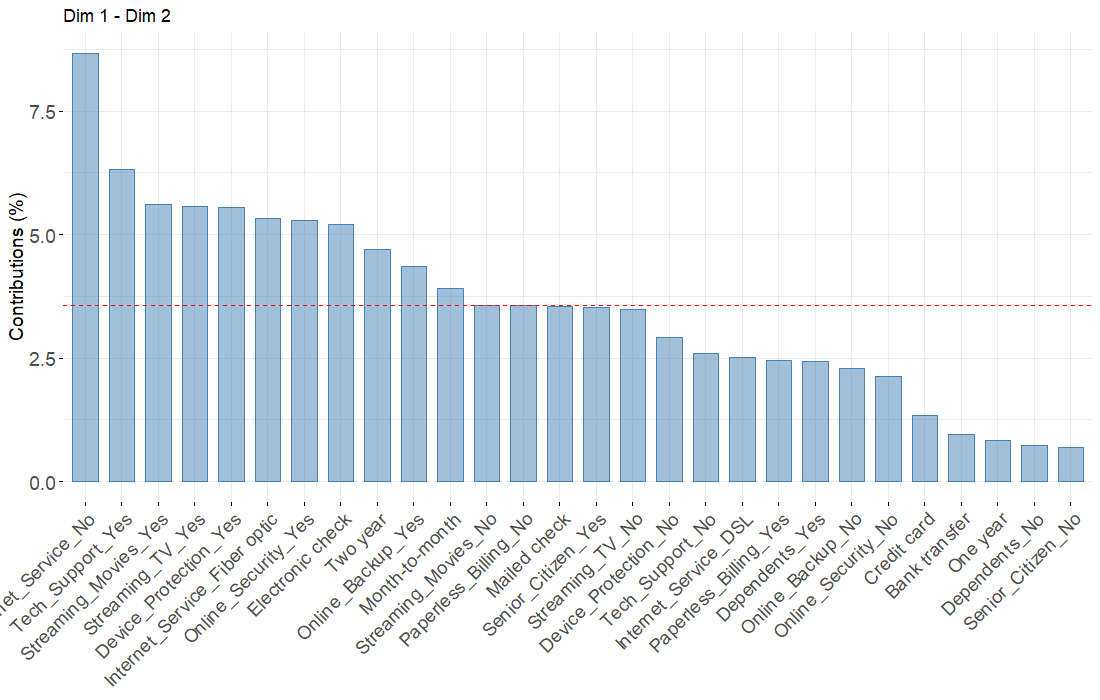
\includegraphics[width=15.28in]{./imgs/mca_contrib_12} 

}

\caption{MCA -  Categories contribution to axes 1 and 2}\label{fig:mcacontrib12}
\end{figure}

\begin{figure}

{\centering 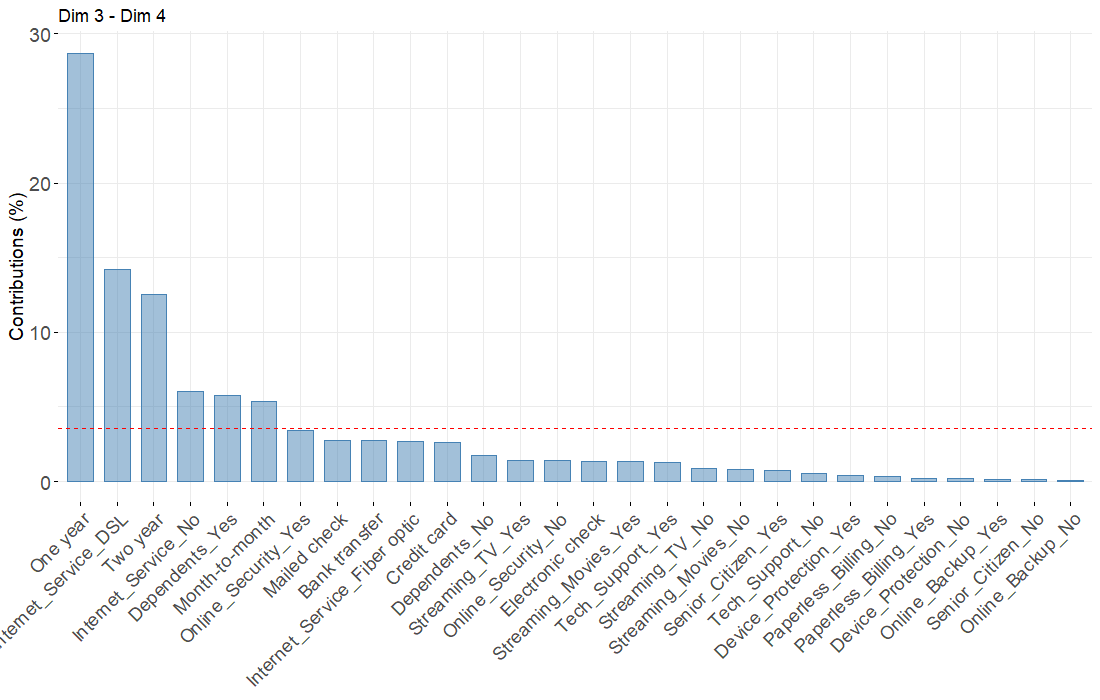
\includegraphics[width=15.28in]{./imgs/mca_contrib_34} 

}

\caption{MCA -  Categories contribution to axes 3 and 4}\label{fig:mcacontrib34}
\end{figure}

\begin{figure}

{\centering 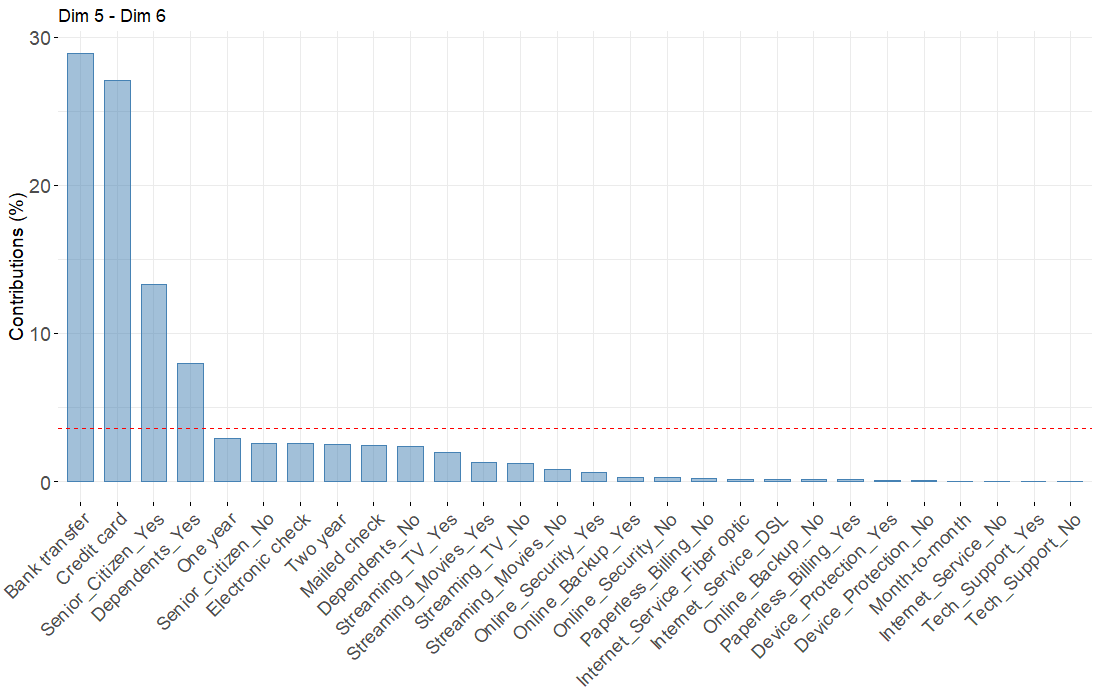
\includegraphics[width=15.28in]{./imgs/mca_contrib_56} 

}

\caption{MCA -  Categories contribution to axes 5 and 6}\label{fig:mcacontrib56}
\end{figure}

\begin{figure}

{\centering 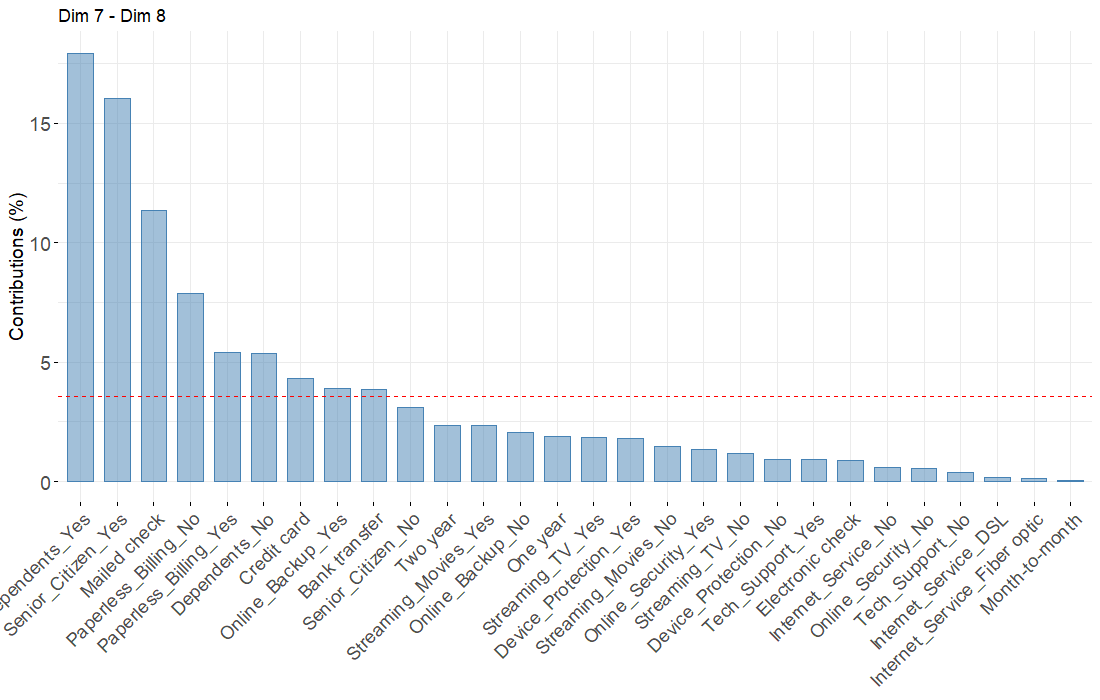
\includegraphics[width=15.28in]{./imgs/mca_contrib_78} 

}

\caption{MCA -  Categories contribution to axes 7 and 8}\label{fig:mcacontrib78}
\end{figure}

\begin{figure}

{\centering 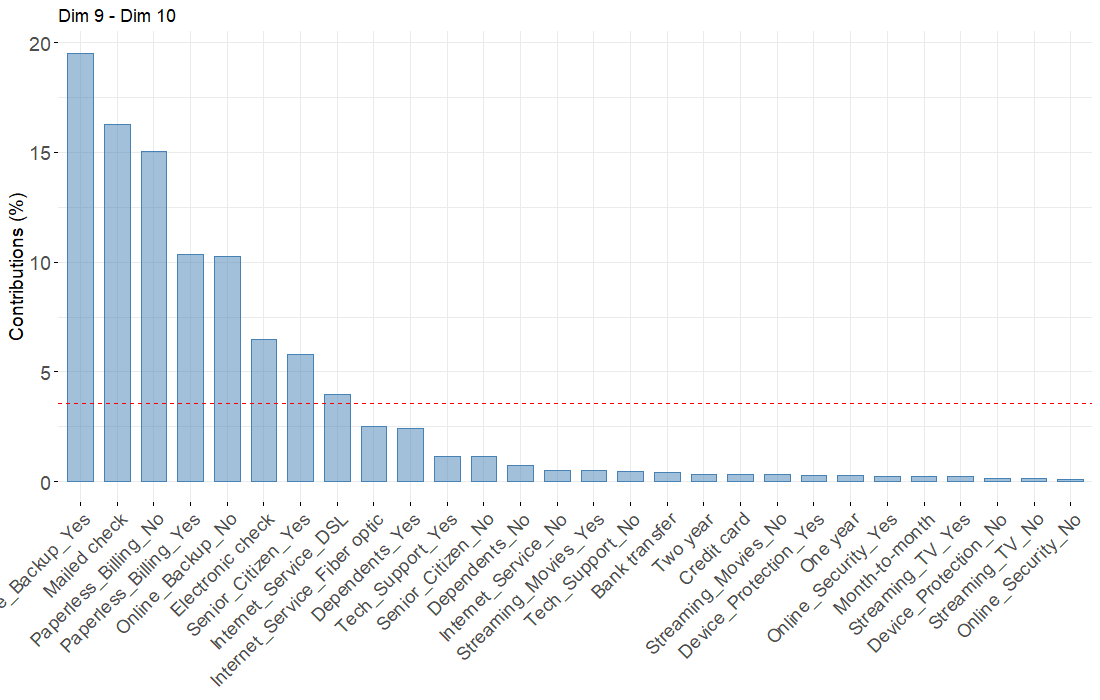
\includegraphics[width=15.28in]{./imgs/mca_contrib_910} 

}

\caption{MCA -  Categories contribution to axes 9 and 10}\label{fig:mcacontrib910}
\end{figure}

\hypertarget{hierarchical-clustering-on-principal-components-1}{%
\section*{Hierarchical clustering on principal components}\label{hierarchical-clustering-on-principal-components-1}}
\addcontentsline{toc}{section}{Hierarchical clustering on principal components}

\hypertarget{cluster-visualisation-1}{%
\subsection*{Cluster visualisation}\label{cluster-visualisation-1}}
\addcontentsline{toc}{subsection}{Cluster visualisation}

\begin{figure}

{\centering 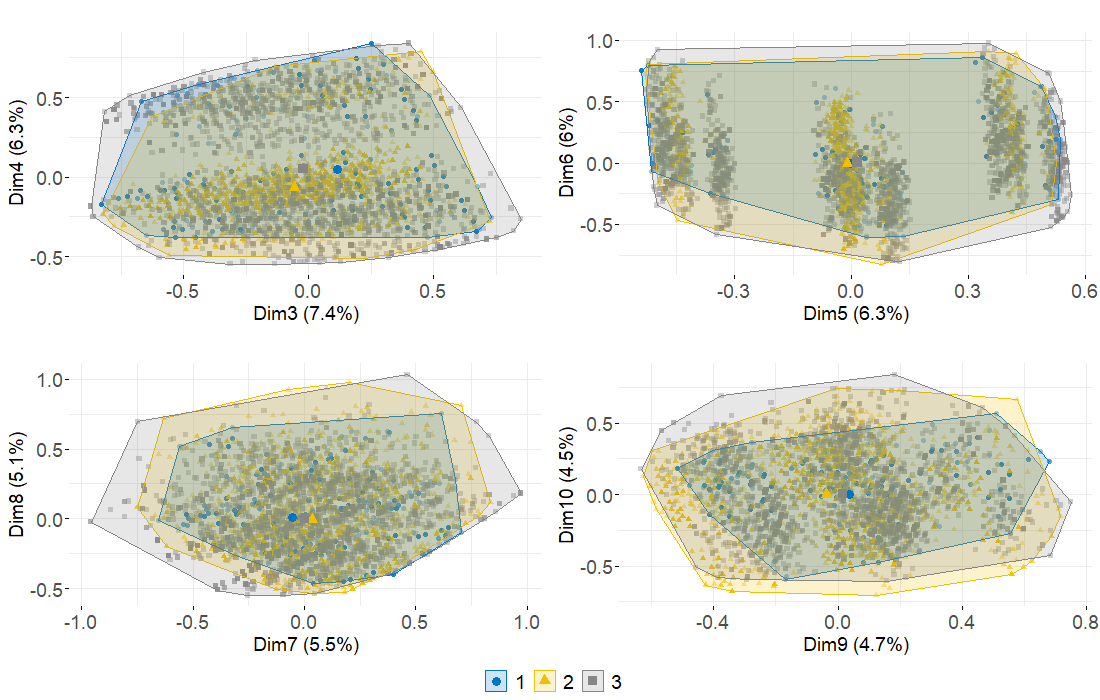
\includegraphics[width=2\linewidth]{./imgs/cluster_plots} 

}

\caption{Cluster visualisation onto MCA axes}\label{fig:clusterplots}
\end{figure}

  \bibliography{biblio.bib,packages.bib}

\end{document}
